\documentclass[
LEEC,			% Use this option to select your DEE degree, options: LEEC, LETI
portuguese,		% Select document language, options: portuguese, english
%draft,			% Uncomment for draft mode (no pictures, no links, overfull hboxes)
]{./class/DEEclass}


% FYI, the following packages are preloaded with the document class:
% longtable, xcolor, graphicx, booktabs, caption, csquotes, hyperref,
% calc, listings, datetime2, siunitx, geometry, enumitem

%%%%%%%%%%%%%%%%%%%%%%%%%%%%%%%%%%%%%%%%%%%%%%%%%%%%%%%%%% extra packages
\usepackage{amsmath}		% the principal package in the AMS-LATEX distribution
\usepackage{amsfonts}		% extended set of fonts for use in mathematics
\usepackage{amssymb}		% adds new symbols to be used in math mode
\usepackage{mathrsfs}		% math fonts, e.g., Laplace
\usepackage{float}			% provides the H float modifier option
\usepackage{multirow}		% tables \multirow command
\usepackage{subcaption}		% enables subfigures
\usepackage{lscape}			% for landscape mode
\usepackage{verbatim}		% new verbatim environment, \begin{comment}...\end{comment}, \verbatiminput

%add extra packages if needed here

%%%%%%%%%%%%%%%%%%%%%%%%%%%%%%%%%%%%%%%%%%%%%%%%%%%%%%%%%% temp packages
\usepackage{lipsum}						% for fake text
%\usepackage[textsize=tiny]{todonotes}   % enable To-do notes, use the option "disable" to hide all notes, usage \todo{}

%\usepackage{draftwatermark}			% prints a watermark overlay, uncomment if needed
%\SetWatermarkText{**DRAFT**}
%\SetWatermarkScale{1}
%\SetWatermarkColor[gray]{0.8}

%%%%%%%%%%%%%%%%%%%%%%%%%%%%%%%%%%%%%%%%%%%%%%%%%%%%%%%%%% settings
\AtBeginDocument{					% Rendered PDF metadata:
\hypersetup{pdftitle=\ttitle} 		% Sets the PDF title to your dissertation title
\hypersetup{pdfauthor=\authorname} 	% Sets the PDF author to your name
}

%%%%%%%%%%%%%%%%%%%%%%%%%%%%%%%%%%%%%%%%%%%%%%%%%%%%%%%%%% user defined macros

%....








		 
%%%%%%%%%%%%%%%%%%%%%%%%%%%%%%%%%%%%%%%%%%%%%%%%%%%%%%%%%%
%\bibliographystyle{plain}
%....
%%%%%%%%%%%%%%%%%%%%%%%%%%%%%%%%%%%%%%%%%%%%%%%%%%%%%%%%%%
%%%%%%%%%%%%%%%%%%%%%%%%%%%%%%%%%%%%%%%%%%%%%%%%%%%%%%%%%%
%%%%%%%%%%%%%%%%%%%%%%%%%%%%%%%%%%%%%%%%%%%%%%%%%%%%%%%%%%
\definecolor{light-gray}{gray}{0.95}
\begin{comment}
%%%%%%%%%%%%%%%%%%ISEP SETTINGS START%%%%%%%%%%%%%%%%%%%%%
\captionsetup{justification=centerlast,font=small,margin=50pt}
\lstset{
language=C,							% choose the language of the code
%basicstyle=\small\ttfamily\color{black},
basicstyle=\footnotesize\ttfamily\color{black},
keywordstyle=\bfseries\color{blue},
numbers=left,						% where to put the line-numbers   
numberstyle=\tiny\color{gray},		% the size of the fonts that are used for the line-numbers
stepnumber=1,						% the step between two line-numbers. If it's 1 each line will be numbered
numbersep=8pt,						% how far the line-numbers are from the code
xleftmargin=2em,					% keep line numbers inside the margins		
frame=tb,							% frame: top and bottom lines
framexleftmargin=1.5em,				% frame: adjusts left margin because the xleftmargin numbers setting
float=!htb,							% if float defined, let Latex manage it
aboveskip=8mm,
belowskip=4mm,
backgroundcolor=\color{light-gray},
commentstyle=\color{red},			% comment style
keywordstyle=\color{blue},			% keyword style
showspaces=false,					% show spaces adding particular underscores
showstringspaces=false,				% underline spaces within strings
showtabs=false,						% show tabs within strings adding particular underscores
tabsize=2,							% sets default tabsize to 2 spaces
captionpos=b,						% sets the caption-position to bottom
breaklines=true,					% sets automatic line breaking
breakatwhitespace=false,			% sets if automatic breaks should only happen at whitespace
escapeinside={\%*}{*)},				% if you want to add a comment within your code
morekeywords={*,var,template,new},	% if you want to add more keywords to the set
stringstyle=\color{orange},
columns=fullflexible
%basicstyle=\small\ttfamily\color{black},
%commentstyle = \ttfamily\color{red},
%keywordstyle=\ttfamily\color{blue},
%backgroundcolor=\color{light-gray},
}
%%%%%%%%%%%%%%%%%%%%ISEP SETTINGS END%%%%%%%%%%%%%%%%%%%%%
\end{comment}
\begin{comment}
\setlistdepth{12}
\newlist{enumitem}{enumerate}{12}
\setlist[enumitem,1]{label=\roman*)}
\setlist[enumitem,2]{label=\alph*)}
\setlist[enumitem,3]{label=\arabic*)}
\setlist[enumitem,4]{label=(\roman*)}
\setlist[enumitem,5]{label=(\alph*)}
\setlist[enumitem,6]{label=(\arabic*)}
\setlist[enumitem,7]{label=\roman*)}
\setlist[enumitem,8]{label=\alph*)}
\setlist[enumitem,9]{label=\arabic*)}
\setlist[enumitem,10]{label=(\roman*)}
\setlist[enumitem,11]{label=(\alph*)}
\setlist[enumitem,12]{label=(\arabic*)}
\end{comment}
%%%%%%%%%%%%%%%%%%%%%%%%%%%%%%%%%%%%%%%%%%%%%%%%%%%%%%%%%%%%%%%%
\begin{comment}
\renewcommand{\labelitemi}{$\bullet$}
\renewcommand{\labelitemii}{$\cdot$}
\renewcommand{\labelitemiii}{$\diamond$}
\renewcommand{\labelitemiv}{$\ast$}
\end{comment}
%%%%%%%%%%%%%%%%%%%%%%%%%%%%%%%%%%%%%%%%%%%%%%%%%%%%%%%%%%%%%%%%
\begin{comment}
\tikzstyle{RECTANGLE_2} = [rectangle, draw, text width=5em, text centered, rounded corners, minimum height=4em]
\tikzstyle{RECTANGLE_3} = [rectangle, rounded corners, minimum width=3cm, minimum height=1cm,text centered, draw=black, fill=red!80]
\tikzstyle{RECTANGLE_4} = [rectangle, draw, fill=blue!20, text width=3cm, text centered, minimum height=4em]
\tikzstyle{RECTANGLE_5} = [rectangle, minimum width=3cm, minimum height=1cm, text centered, text width=3cm]
\tikzstyle{RECTANGLE_6} = [rectangle, draw, fill=blue!20, text width=5em, text centered, rounded corners, minimum height=4em]
\tikzstyle{RECTANGLE_7} = [rectangle, draw, fill=blue!20, text width=5em, text centered, rounded corners, minimum height=4em]
\tikzstyle{RECTANGLE_8} = [rectangle, draw, align=left, fill=blue!20]
\tikzstyle{RECTANGLE_1} = [rectangle, rounded corners, minimum width=1cm, minimum height=1cm,text centered, draw=black, fill=green!%30]
\tikzstyle{DIAMOND_1} = [diamond, draw, fill=blue!20, text width=4.5em, text badly centered, node distance=4cm, inner sep=0pt]
\tikzstyle{DIAMOND_2} = [diamond, minimum width=3cm, minimum height=1cm, text centered, draw=black, fill=green!30]
\tikzstyle{DIAMOND_3} = [diamond, draw, text width=4.5em, text badly centered, node distance=3cm, inner sep=0pt]
\tikzstyle{DIAMOND_4} = [diamond, draw, fill=blue!20, text width=4.5em, text badly centered, node distance=3cm, inner sep=0pt]
\tikzstyle{DIAMOND_5} = [diamond, draw, fill=blue!20, text width=4.5em, text badly centered, node distance=3cm, inner sep=0pt]
\tikzstyle{DIAMOND_6} = [diamond, draw, fill=blue!20, text width=4.5em, text badly centered, node distance=4cm, inner sep=0pt]
\tikzstyle{DIAMOND_7} = [diamond, draw, align=left, fill=blue!20]
\tikzstyle{ELLIPSE_1} = [draw, ellipse,fill=red!20, node distance=3cm, minimum height=2em]
\tikzstyle{ELLIPSE_2} = [draw, ellipse,fill=red!20, node distance=3cm, minimum height=2em]
\tikzstyle{ELLIPSE} = [draw, ellipse,fill=red!20, node distance=3cm, minimum height=2em]
\tikzstyle{TRAPEZIUM_1} = [trapezium,trapezium left angle=70,trapezium right angle=-70,minimum height=0.6cm, draw, fill=blue!20, text width=4.5em, text badly centered, node distance=3cm, inner sep=0pt]
\tikzstyle{TRAPEZIUM_2} = [trapezium, trapezium left angle=70, trapezium right angle=110, minimum width=3cm, minimum height=1cm, text centered, draw=black, fill=blue!30]
\tikzstyle{TRAPEZIUM_3} = [trapezium,trapezium left angle=70,trapezium right angle=-70,minimum height=0.6cm, draw, fill=blue!20, text width=4.5em, text badly centered, node distance=3cm, inner sep=0pt]
\tikzstyle{ARROW} = [thick,->,>=stealth]
\tikzstyle{LINE} = [draw, -latex']
\tikzstyle{MYLINE} = [draw, ->,  thick, shorten <=4pt, shorten >=4pt]
\tikzstyle{TEXT_1}=[draw,text centered,minimum size=6em,text width=5.25cm,text height=0.34cm]
\tikzstyle{TEXT_2}=[draw,text centered,minimum size=2em,text width=2.75cm,text height=0.34cm]
\tikzstyle{TEXT_3}=[draw,minimum size=2.5em,text centered,text width=3.5cm]
\tikzstyle{TEXT_4}=[draw,minimum size=3em,text centered,text width=6.cm]
\tikzstyle{CIRCLE_1}=[draw,shape=circle,inner sep=2pt,text centered, node distance=3.5cm]
\tikzstyle{CIRCLE_2}=[draw,shape=circle,inner sep=4pt,text centered, node distance=3.cm]
\end{comment}
\begin{comment}
%%%%%%%GANTT 1%%%%%%%
\newganttchartelement*{mymilestone}{
mymilestone/.style={
shape=isosceles triangle,
inner sep=0pt,
draw=cyan,
top color=white,
bottom color=cyan!50
},
mymilestone incomplete/.style={
/pgfgantt/mymilestone,
draw=yellow,
bottom color=yellow!50
},
mymilestone label font=\slshape,
mymilestone left shift=0pt,
mymilestone right shift=0pt
}
\newgantttimeslotformat{stardate}{%
\def\decomposestardate##1.##2\relax{%
\def\stardateyear{##1}\def\stardateday{##2}%
}%
\decomposestardate#1\relax%
\pgfcalendardatetojulian{\stardateyear-01-01}{#2}%
\advance#2 by-1\relax%
\advance#2 by\stardateday\relax%
}
\end{comment}
%%%%%%%GANTT 2%%%%%%%
%%%%%%%%%%%%%%%%%%%%%%%%%%%%%%%%%%%%%%%%%%%%%%%%%%%%%%%%%%
%\addto{\captionsportuguese}{\renewcommand*\contentsname{\'{I}ndice}}
%\addto{\captionsportuguese}{\renewcommand{\appendixname}{Anexo}}
%\addto{\captionsportuguese}{\renewcommand{\bibname}{Refer\^{e}ncias}}
%\addto{\captionsportuguese}{\renewcommand*\lstlistingname{Listagen}}
%\addto{\captionsportuguese}{\renewcommand*\lstlistlistingname{Listagens}}
%\addto{\captionsportuguese}{\renewcommand*\acronymname{Acrónimos}}
%%%%%%%%%%%%%%%%%%%%%%%%%%%%%%%%%%%%%%%%%%%%%%%%%%%%%%%%%%
%\newtheorem{theorem}{Theorem}
%\newtheorem{lemma}{Lemma}
%\newtheorem{definition}{Defini\c{c}\~{a}o}
%\newtheorem{notation}{Notation}
%%%%%%%%%%%%%%%%%%%%%%%%%%%%%%%%%%%%%%%%%%%%%%%%%%%%%%%%%%
\makeatletter
\renewcommand{\@makechapterhead}[1]{%
	\vspace*{50 pt}%
	{\setlength{\parindent}{0pt} \raggedright \normalfont
		\bfseries\Huge\thechapter.\ #1
		\par\nobreak\vspace{40 pt}}}
\makeatother
%%%%%%%%%%%%%%%%%%%%%%%%%%%%%%%%%%%%%%%%%%%%%%%%%%%%%%%%%%
%\renewcommand\thesection{\arabic{section}}
%\renewcommand\thesubsection{\thesection.\arabic{subsection}}
%%%%%%%%%%%%%%%%%%%%%%%%%%%%%%%%%%%%%%%%%%%%%%%%%%%%%%%%%%
\newcommand{\minipagespace}[1]{{\newline \vspace{#1cm} \newline}}
\newcommand{\tablespace}[1]{{\vspace{#1cm}}}
\newcommand{\figurespace}[1]{{\vspace{#1cm}}}
\newcommand{\listingspace}[1]{{\vspace{#1cm}}}
%%%%%%%%%%FIX SECTION NUMBERING IN CASE REPORT%%%%%%%%%%%%
%\renewcommand\thesection{\arabic{section}}
%\renewcommand\thesubsection{\thesection.\arabic{subsection}}
%\renewcommand\thesubsubsection{\thesection.\thesubsection.\arabic{subsubsection}}
%%%%%%%%%%%%%%%%%%%%%%%%%%%%%%%%%%%%%%%%%%%%%%%%%%%%%%%%%%
\newcolumntype{L}[1]{>{\raggedright\arraybackslash}p{#1}}
\newcolumntype{C}[1]{>{\centering\arraybackslash}p{#1}}
\newcolumntype{R}[1]{>{\raggedleft\arraybackslash}p{#1}}
%%%%%%%%%%%%%%%%%%%%%%%%%%%%%%%%%%%%%%%%%%%%%%%%%%%%%%%%%%
\lstnewenvironment{java}[1][]{%
	\lstset{language=Java,#1}%
}{}
\newcommand*{\incjava}[1][]{%
	\lstinputlisting[{language=Java,#1}]%
}
%%%%%%%%%%%%%%%%%%%%%%%%%%%%%%%%%%%%%%%%%%%%%%%%%%%%%%%%%%
\begin{comment}
\lstloadlanguages{C}
\lstset{
basicstyle=\small\ttfamily\color{black},
commentstyle = \ttfamily\color{red},
keywordstyle=\ttfamily\color{blue},
stringstyle=\color{orange},
backgroundcolor=\color{light-gray},
columns=fullflexible
}
\end{comment}
%%%%%%%%%%%%%%%%%%%%%%%%%%%%%%%%%%%%%%%%%%%%%%%%%%%%%%%%%%

%%%%%%%%%%%%%%%%%%%% REPORT INFORMATION %%%%%%%%%%%%%%%%%%

\reporttitle{Balança Digital} % Your report title

%\reportsubtitle{Com um Subtítulo se Necessário} % and subtitle, uncomment if needed
%\subdate{Janeiro, 2021} % Uncomment for a static submission date, or leave it as a comment for automatic date (month+year) 

\author{Sergio Manuel Salazar dos Santos}	% Your name
\studentnumber{1020881}	% Your student number
\studentemail{1020881@isep.ipp.pt}	% Your student email address  

\advisor{Isabel Gonçalves Vaz}{igv@isep.ipp.pt}	% Your ISEP advisor name and email
%\coadvisor{Nome do Coorientador}{xxx@isep.ipp.pt}	% Your ISEP co-advisor name and email, comment this line if not needed
%\company{Nome da Empresa, Lda.}	% The company name where you developed your work, comment this line if not needed
%\supervisor{Nome do Orientador da Empresa}{xxx@emailaddress.com} % Your company supervisor name, comment this line if not needed

%%%%%%%%%%%%%%%% USER DEFINED LISTS %%%%%%%%%%%%%%%%%%%%%%
\makeglossaries						% Consider the following files in the 'front' folder:
%---------------------------------------------------------
%	GLOSSARY
%---------------------------------------------------------
% Only the used entries will be displayed in the printed list, ie, you need to used a term at least once
% In italic if not in the main document language
% terms definition usage:
% \newglossaryentry{<tag>}{name={<term>},description={<description of the term>}}
%\makeglossaries
\newglossaryentry{gloss}{
name={glossário}, 
description={é uma lista alfabética de termos de um determinado domínio de conhecimento com a definição desses mesmos termos.},
}
\newglossaryentry{pack}{
name={\textit{package}}, 
description={é um ficheiro ou conjunto de ficheiros que contêm comandos \LaTeX{} extra que adicionam novas funcionalidades de estilo ou modificam aquelas já existentes.},
sort={package}	%needed for sorting when using LaTeX commands in the 'name' field
}
\newglossaryentry{lipsum}{
name={\textit{Lorem Ipsum}}, 
description={é uma sequência de palavras, geralmente latinas, utilizada para preencher o espaço destinado a texto numa publicação, por forma a testar as opções de formatação e edição e o arranjo dos elementos gráficos antes da inserção do conteúdo.},
sort={Lorem Ipsum}
}
%%%%%%%%%%%%%%%%%%%%%%%%%%%%%%%%%%%%%%%%%%%%%%%%%%%%%%%%%%%%%%%%
\newglossarystyle{mylong}{%
	\setglossarystyle{long}%
	\renewenvironment{theglossary}%
	{\begin{longtable}[l]{@{}p{\dimexpr 3cm-\tabcolsep}p{.7\hsize}}}% <-- change the value here
		{\end{longtable}}%
}
\newglossaryentry{latex}
{
	name=latex,
	description={Is a mark up language specially suited 
		for scientific documents}
}
\newglossaryentry{maths}
{
	name=mathematics,
	description={Mathematics is what mathematicians do}
}
\newglossaryentry{formula}{
	name=formula,
	description={A mathematical expression}
}
\newglossaryentry{Biofouling}{
	name=Biofouling,description={Some description}
}
\newglossaryentry{symb:Pi}{
	name=\ensuremath{\pi},
	description={Geometrical value}
}
%%%%%%%%%%%%%%%%%%%%%%%%%%%%%%%%%%%%%%%%%%%%%%%%%%%%%%%%%%
			% Edit to define your glossary entries list
%----------------------------------------------------------------------------------------
%	ACRONYMS LIST
%----------------------------------------------------------------------------------------

% Only the used entries will be displayed in the printed list, ie, you need to used a acronym at least once
% Full name in italic if not in the main document language

%acronym definition usage:
%\newacronym{<tag>}{<acronym>}{<full name>}

\newacronym{gcd}{GCD}{\textit{Greatest Common Divisor}}
\newacronym{lcm}{LCM}{\textit{Least Common Multiple}}
\newacronym{ide}{IDE}{\textit{Integrated Development Environment}}
\newacronym{cots}{COTS}{\textit{Components Of The Shelf}}
\newacronym{cpu}{CPU}{\textit{Communications Processor Unit}}
\newacronym{crc}{CRC}{\textit{Cyclic Redundancy Check}}
\newacronym{eeprom}{EEPROM}{\textit{Electrically Erasable Programmable Read-Only Memory}}
\newacronym{fcs}{FCS}{\textit{Frame Check Sequence}}
\newacronym{fifo}{FIFO}{\textit{First In First Out}}
\newacronym{mems}{MEMS}{\textit{Microelectromechanical Systems}}
\newacronym{rom}{ROM}{\textit{Read-only Memory}}
\newacronym{ram}{RAM}{\textit{Random-access Memory}}
\newacronym{isp}{ISP}{\textit{In-System Programming}}
\newacronym{jtag-dp}{JTAG-DP}{\textit{Joint Test Action Group}}
\newacronym{jtag}{JTAG}{\textit{Joint Test Action Group}}
\newacronym{swd-dp}{SWD-DP}{\textit{Serial Wire Debug}}
\newacronym{iap}{IAP}{\textit{in-application programming}}
\newacronym{icp}{ICP}{\textit{in-circuit programming}}
\newacronym{pvp}{PVP}{Preço de Venda ao Público}
\newacronym{atmel-ice}{ATMEL-ICE}{\textit{Development tool for debugging and programming ARM \textsuperscript{\textregistered} Cortex \textsuperscript{\textregistered} -M based Atmel \textsuperscript{\textregistered} SAM and Atmel AVR \textsuperscript{\textregistered} microcontrollers with On-Chip Debug capability}}
\newacronym{msb}{MSB}{\textit{Most Significant Bit}}
\newacronym{mcu}{MCU}{\textit{Microcontroller Unit}}
\newacronym{adc}{ADC}{\textit{Analog to Digital Converter}}
\newacronym{lcd}{LCD}{\textit{Liquid Crystal Display}}
\newacronym{rtos}{RTOS}{\textit{Real Time Operating System}}
\newacronym{idc}{IDC}{\textit{insulation-displacement contact}}
\newacronym{sram}{SRAM}{\textit{Static Random-Access Memory}}
\newacronym{gpr}{GPR}{\textit{General Purpose Registers}}
\newacronym{sfr}{SFR}{\textit{Special Function Registers}}
\newacronym{risc}{RISC}{\textit{Reduced Instruction Set Computer ou Reduced COMPLEXITY Instruction Set Computer}}
\newacronym{pic}{PIC}{\textit{Peripheral Interface Controller}}
\newacronym{flash}{FLASH}{\textit{electronic non-volatile computer memory storage medium}}
\newacronym{pwm}{PWM}{\textit{Pulse-width modulation}}
\newacronym{spi}{SPI}{\textit{Serial Peripheral Interface}}
\newacronym{usart}{USART}{\textit{Universal Synchronous/Asynchronous Receiver/Transmitter}}
\newacronym{twi}{TWI}{\textit{Two-Wire Interface}}
\newacronym{rtc}{RTC}{\textit{Real Time Counter}}
\newacronym{mips}{MIPS}{\textit{Million Instructions Per Second}}
\newacronym{e2prom}{E2PROM}{\textit{Electrically Erasable Programmable Read-Only Memory}}
\newacronym{pcb}{PCB}{\textit{Printed Circuit Board}}
\newacronym{wys}{WYSIWYG}{\textit{What You See Is What You Get}}
\newacronym{dee}{DEE}{Departamento de Engenharia Electrotécnica}
\newacronym{api}{API}{\textit{Application Programming Interface}}
\newacronym{ascii}{ASCII}{\textit{American Standard Code for Information Interchange}}
\newacronym{html}{HTML}{\textit{HyperText Markup Language}}
\newacronym{isep}{ISEP}{Instituto Superior de Engenharia do Porto}
\newacronym{leec}{LEEC}{Licenciatura em Engenharia Eletrot\'{e}cnica e de Computadores}
\newacronym{leti}{LETI}{Licenciatura em Engenharia de Telecomunicações e Informática}
\newacronym{usb}{USB}{\textit{Universal Serial Bus}}
\newacronym{pdf}{PDF}{\textit{Portable Document Format}}
			% Edit to define your acronyms entries list
%----------------------------------------------------------------------------------------
%	SYMBOLS LIST
%----------------------------------------------------------------------------------------

% terms definition usage:
% \newglossaryentry{<tag>}{
% name={<symbol>},
% sort={<text for the alphabetical sorting>},
% description={<description of the symbol>},
% unit={<units to display>},
% type=symbolslist}

\newglossaryentry{f}{
name={\ensuremath{f}},
sort={f},
description={força},
unit=\si{\newton},
type=symbolslist}

\newglossaryentry{i}{
name={\ensuremath{i}},
sort={i},
description={corrente},
unit=\si{\ampere},
type=symbolslist}

\newglossaryentry{m}{
name=\ensuremath{M},
sort={m},
description={massa},
unit=\si{\kilogram},
type=symbolslist}

\newglossaryentry{p}{
name=\ensuremath{P},
sort={p},
description={potência},
unit=\si{\watt},
type=symbolslist}

\newglossaryentry{theta}{
name=\ensuremath{\theta},
sort={z1},
description={deslocamento angular},
unit=\si{\radian},
type=symbolslist}

\newglossaryentry{omega}{
name=\ensuremath{\omega},
sort={z2},
description={velocidade angular},
unit=\si{\radian\per\second},
type=symbolslist}

\newglossaryentry{x}{
name=\ensuremath{x},
sort={x},
description={deslocamento},
unit=\si{\meter},
type=symbolslist}

% Greek: alpha,beta,gamma,delta,epsilon,zeta,eta,theta,iota,kappa,lambda,mu,nu,xi,omikron,pi,rho,sigma,tau,upsilon,phi,chi,psi,omega

				% Edit to define your symbols entries list
%\glsaddall
%%%%%%%%%%%%%%%%%%%%%%%%%%%%%%%%%%%%%%%%%%%%%%%%%%%%%%%%%%
\begin{document}
\frontmatter

%---------------------------------------------------------
%	TITLE PAGES
%---------------------------------------------------------
\pagestyle{plain} % Default to the plain heading style until the thesis style is called for the body content
\printcoverpage
\printaftercoverpage
\cleardoublepage
%%%%%%%%%%%%%%%%%%%%%%%%%%%%%%%%%%%%%%%%%%%%%%%%%%%%%%%%%%














%%%%%%%%%%%%%%%%%%%%%%%% FRONTMATTER %%%%%%%%%%%%%%%%%%%%%
%%----------------------------------------------------------------------------------------
%	DEDICATION
%----------------------------------------------------------------------------------------

\dedicatory{
(Opcional) Poderá usar esta secção para dedicar o trabalho a alguém\ldots
} 

%---------------------------------------------------------
%	ACKNOWLEDGEMENTS
%---------------------------------------------------------
\begin{acknowledgements}
Ao \ac{isep}, como instituto com fortes valores e princípios, que permaneçam no bom caminho, criando cada vez mais formandos aptos para enfrentar os desafios do futuro, e crescer de forma positiva. Agradecer aos docentes que partilharam seus conhecimentos e nos permitiu desenvolver as competências necessárias para atingir os nossos objetivos. \\
\\
Um especial agradecimento ao orientador do Projeto/Estagio Engª Isabel Gonçalves Vaz, pelos conselhos e opiniões.
\end{acknowledgements}
%%%%%%%%%%%%%%%%%%%%%%%%%%%%%%%%%%%%%%%%%%%%%%%%%%%%%%%%%%

%----------------------------------------------------------------------------------------
%	ABSTRACT PAGES
%----------------------------------------------------------------------------------------

% IMPORTANT NOTE: the abstract must always be written in two languages. If the report
% is written in Portuguese you have selected 'portuguese' as the language in the document class.
% Therefore, the portuguese version of the abstract must come first, so write it in the
% below area denoted by 'MAIN LANGUAGE ABSTRACT'. The english version follows in the
% 'SECOND LANGUAGE ABSTRACT' section.
% If the report is written in English, first will come the abstract in English
% ('MAIN LANGUAGE ABSTRACT') and then in Portuguese ('SECOND LANGUAGE ABSTRACT').

\begin{abstract}
%%%%%%%%%%%%%%%%%%%%%%%%%%%%%% MAIN LANGUAGE ABSTRACT %%%%%%%%%%%%%%%%%%%%%%%%%%%%%%%%%%

\par O projeto proposto passa por fazer uma balança, utilizando um micro controlador(\textit{Embedded System}). Uma célula carga será o sensor de conversão da diferença de potencial obtida de uma ponte \textit{Wheatstone} pela existencia de uma massa a pesar sobre a célula de carga, gerando um sinal proporcional ao seu peso.
\\
\\
Após obter este sinal, será ligado a um amplificador \ac{adc} dedicado para este tipo de funcionalidade, com 24 bits de resolução, com amplificação programável e com uma taxa de transferência fisicamente (\textit{hardware}) programada. Este amplificador é designado por \textbf{HX711}, e possui um protocolo de comunicação que lhe é próprio. Depois esta comunicação serie vai ser entregue a um \ac{mcu}.
\\
\\
A programação do \acrshort{mcu}, o código das livrarias e ou drivers será implementada em linguagem \textbf{C}. O objetivo é obter uma balança funcional de fácil utilização e calibração economicamente viável, desta forma uma balança acessível e prática.
%%A massa é uma das grandezas fundamentais [\textbf{LMT}] dai minha opção por apostar neste projeto devido a toda a física estar envolvida ao seu redor.
\\
\\
Este trabalho é orientado para quem tem alguns conhecimentos básicos de eletrotecnia, com orientação para a eletrónica e programação.

%----------------------------------------------------------------------------------------

\vspace*{10mm} 
\noindent
\textbf{\keywordslabel}: \textit{Strain Gauge}, \textit{Load Cell}, Amplificador, Código, Programação, \textit{Embedded System} .

%%%%%%%%%%%%%%%%%%%%%%%%% END OF THE MAIN LANGUAGE ABSTRACT %%%%%%%%%%%%%%%%%%%%%%%%%%%%%%
\end{abstract}
\begin{secondlangabstract}
%%%%%%%%%%%%%%%%%%%%%%%%%%%%%% SECOND LANGUAGE ABSTRACT %%%%%%%%%%%%%%%%%%%%%%%%%%%%%%%%%%

\par The proposed project is to build a wheighing scale using a microcontroller, an Embedded system.
\\
\\
A load cell is what is going to be used to convert the measured wheight into a potencial difference with a wheatstone configuration, generating a proportional signal.
\\
\\
After obtaing this signal it is going to be connected to a load cell amplifier with a \ac{adc} dedicated for this type of application, it has a 24 bit resolution, programable amplification and sampling rate fisically programmmable, this is the \textbf{HX711} chip, having a proprietary communication protocol.
This information then will be passed to the microcontroller.
\\
\\
The \ac{mcu} programming code, libraries and or drivers are to be implemented using the \textbf{C} language. The objective of this project is to get a functional wheighing scale easy to use and to calibrate economically viable, in order to have a practical wheight scale.
\\
\\
This work is targeted to a public with some basic electrical knowledge with electronic and programming background.


%----------------------------------------------------------------------------------------

\vspace*{10mm} 
\noindent
\textbf{\keywordslabel}: Strain Gauge, Load Cell, Amplifier, Code, Programming, Embedded System.

%%%%%%%%%%%%%%%%%%%%%%%%%% END OF THE SECOND LANGUAGE ABSTRACT %%%%%%%%%%%%%%%%%%%%%%%%%%%%%
\end{secondlangabstract}


%---------------------------------------------------------
%	FONTMATTER LISTS
%---------------------------------------------------------
\pdfbookmark[0]{\contentsname}{toc}
\tableofcontents 	
\glsresetall
%---------------------------------------------------------
% Of the following lists, comment the ones you will not use in your document
\listoffigures 			% Prints the list of figures
\listoftables 			% Prints the list of tables
\printlistoflistings	% Prints the list of listings (source code segments)
\printlistofterms		% Prints the list of USED terms (glossary)
%\printglossaries
\printlistofacronyms{XXXXXXXXI} % Prints the list of USED acronyms
\printglossary[title=Acrónimos, style=mylong, type=\acronymtype]
% Change the argument with random letters to adjust the left alignment of the acronyms full name column
%\printlistofsymbols		% Prints the list of ALL defined symbols
%%%%%%%%%%%%%%%%%%%%%%%%%%%%%%%%%%%%%%%%%%%%%%%%%%%%%%%%%%

%%%%%%%%%%%%%%%%%%%%%%%%% MAINMATTER%%%%%%%%%%%%%%%%%%%%%%
\mainmatter 
\pagestyle{plain} %%thesis, empty, plain

%%%%%%%%%%%%%%%%%%%%%%%%%%%%%%%%%%%% Chapter Template

\chapter{Introdução} 	% Main chapter title
\label{Chapter1} 		% For referencing the chapter elsewhere, usage \ref{Chapter1}

%%%%%%%%%%%%%%%%%%%%%%%%%%%%%%%%%%%%

Este documento pretende guiar o Estudante na elaboração do relatório de Projeto/Estágio, do 3º ano da \ac{leec} e da \ac{leti}, do \ac{dee}, do \ac{isep}.

O autor deverá ter em consideração as seguintes regras gerais na elaboração do documento:

\begin{itemize}
	\item É fundamental refletir, antes de escrever, sobre a substância do que se pretende transmitir.
	\item Deve organizar o texto evitando a excessiva divisão do mesmo em tópicos que supostamente se enquadram no tema principal da secção a que pertencem. A excessiva especialização pode ser reveladora de falta de conhecimento e/ou reflexão. Neste sentido, deve, antes de iniciar a escrita, exercitar-se em refinar a organização do texto com o intuito de evitar que existam mais do que 2 níveis de ``profundidade'' em cada secção (respetivamente, subsecção e sub-subsecção). Note que o número de capítulos, secções e subsecções do presente documento não é vinculativo nem mesmo indicativo, apenas serve os propósitos do mesmo.
	\item O documento deve ser redigido em português ou inglês com um estilo adequado (evite o tom coloquial, lugares comuns e chavões) e correto do ponto de vista gramatical (quer do ponto de vista sintático quer semântico).
	\item Tenha especial cuidado com o uso de adjetivos (facilmente conduzem ao exagero), advérbios (nada, ou quase nada, acrescentam) e sinais de pontuação (em especial o uso correto das vírgulas).
	\item O estilo adotado para a redação deve ser coerente com as exigências de um trabalho científico encontrado em publicações impressas.
	\item De uma forma genérica deve usar a 3ª pessoa do singular (eventualmente do plural), exceção feita aos locais onde tal é claramente desajustado, por exemplo, na secção dos agradecimentos.
	\item Usar o estilo \textit{itálico} sempre que são utilizados termos em línguas diferentes da língua adotada no relatório.
	\item O uso de acrónimos implica que na 1ª vez que são utilizados se apresentem por extenso, colocando entre parênteses a respetiva sigla que se passará a usar. No entanto, é sempre possível, mais à frente no texto, e por uma questão de legibilidade, repetir o significado do acrónimo. Todos os acrónimos devem ser apresentados por ordem alfabética na secção ``Lista de Acrónimos''.
	\item O uso correto de unidades, seus múltiplos e submúltiplos.
	\item As imagens e tabelas devem, por princípio, aparecer no topo ou no fundo da página. A legendas surgem imediatamente após as figuras e listagens. No caso das tabelas as legendas antecedem as mesmas.
	\item Todas as figuras, tabelas e restantes listagens devem ser mencionadas no texto por forma a que fiquem enquadradas nas ideias transmitidas pelo autor. Esta referência, regra geral, deverá ser feita antes da ocorrência da figura, tabela ou listagem.
	\item Deve indicar ao longo do texto as referências documentais usadas, em especial nas citações (puras ou literais), assinaladas com a utilização de aspas, como também no caso de reutilização de gráficos, figuras, tabelas, fórmulas, etc., de outras fontes.
\end{itemize}

De uma forma já mais específica, neste primeiro capítulo obrigatório (``Introdução'') o autor deve:

\begin{itemize}
	\item contextualizar a proposta de trabalho no âmbito da empresa, de um outro trabalho já realizado, do ponto de vista científico e/ou tecnológico, etc.,
	\item apresentar de forma clara os objetivos que se propõe atingir,
	\item descrever de forma sucinta, mas objetiva, a solução preconizada ou a hipótese colocada,
	\item apresentar de forma resumida, mas clara, os desenvolvimentos efetuados,
	\item identificar como foi validada e avaliada a solução encontrada,
	\item descrever a organização do documento.
\end{itemize}

Sem ser exigida nenhuma organização em particular para este capítulo, são indicadas a título de exemplo 4 secções (com texto \gls{lipsum}) que podem ser incorporadas nesta parte do documento: Contextualização, Descrição do Projeto, Calendarização e Organização do Relatório. 	

%%%%%%%%%%%%%%%%%%%%%%%%%%%%%%%%%%%% SECTION 1

\section{Contextualização}
\label{sec:Ch1.1}

\lipsum[1] % inserts fake text, to be removed in your dissertation

%%%%%%%%%%%%%%%%%%%%%%%%%%%%%%%%%%%% SECTION 2

\section{Descrição do Projeto}
\label{sec:Ch1.2}

\lipsum[2]

%%%%%%%%%%%%%%%%%%%%%%%%%%%%%%%%%%%% SUBSECTION 1

\subsection{Objetivos}
\label{sub:Ch1.2.1}

\lipsum[2]

%%%%%%%%%%%%%%%%%%%%%%%%%%%%%%%%%%%% SECTION 3

\section{Calendarização}
\label{sec:Ch1.3}

\lipsum[1]
% you could use the pgfgantt package: https://ctan.org/pkg/pgfgantt


%%%%%%%%%%%%%%%%%%%%%%%%%%%%%%%%%%%% SECTION 4

\section{Organização do Relatório}
\label{sec:Ch1.4}

\lipsum[2]




\chapter{Balança Digital}
\label{Chapter2}
Para o desenvolvimento deste projeto, foi criado um kit de desenvolvimento para facilitar sua implementação, testar, efetuar alterações e melhoramentos.
\\
\\
Abaixo pode-se ver a montagem em esqueleto do equipamento utilizado na \textit{figura} \ref{Kit_Desenvolvimento_2},
\begin{figure}[H]
	\centering
	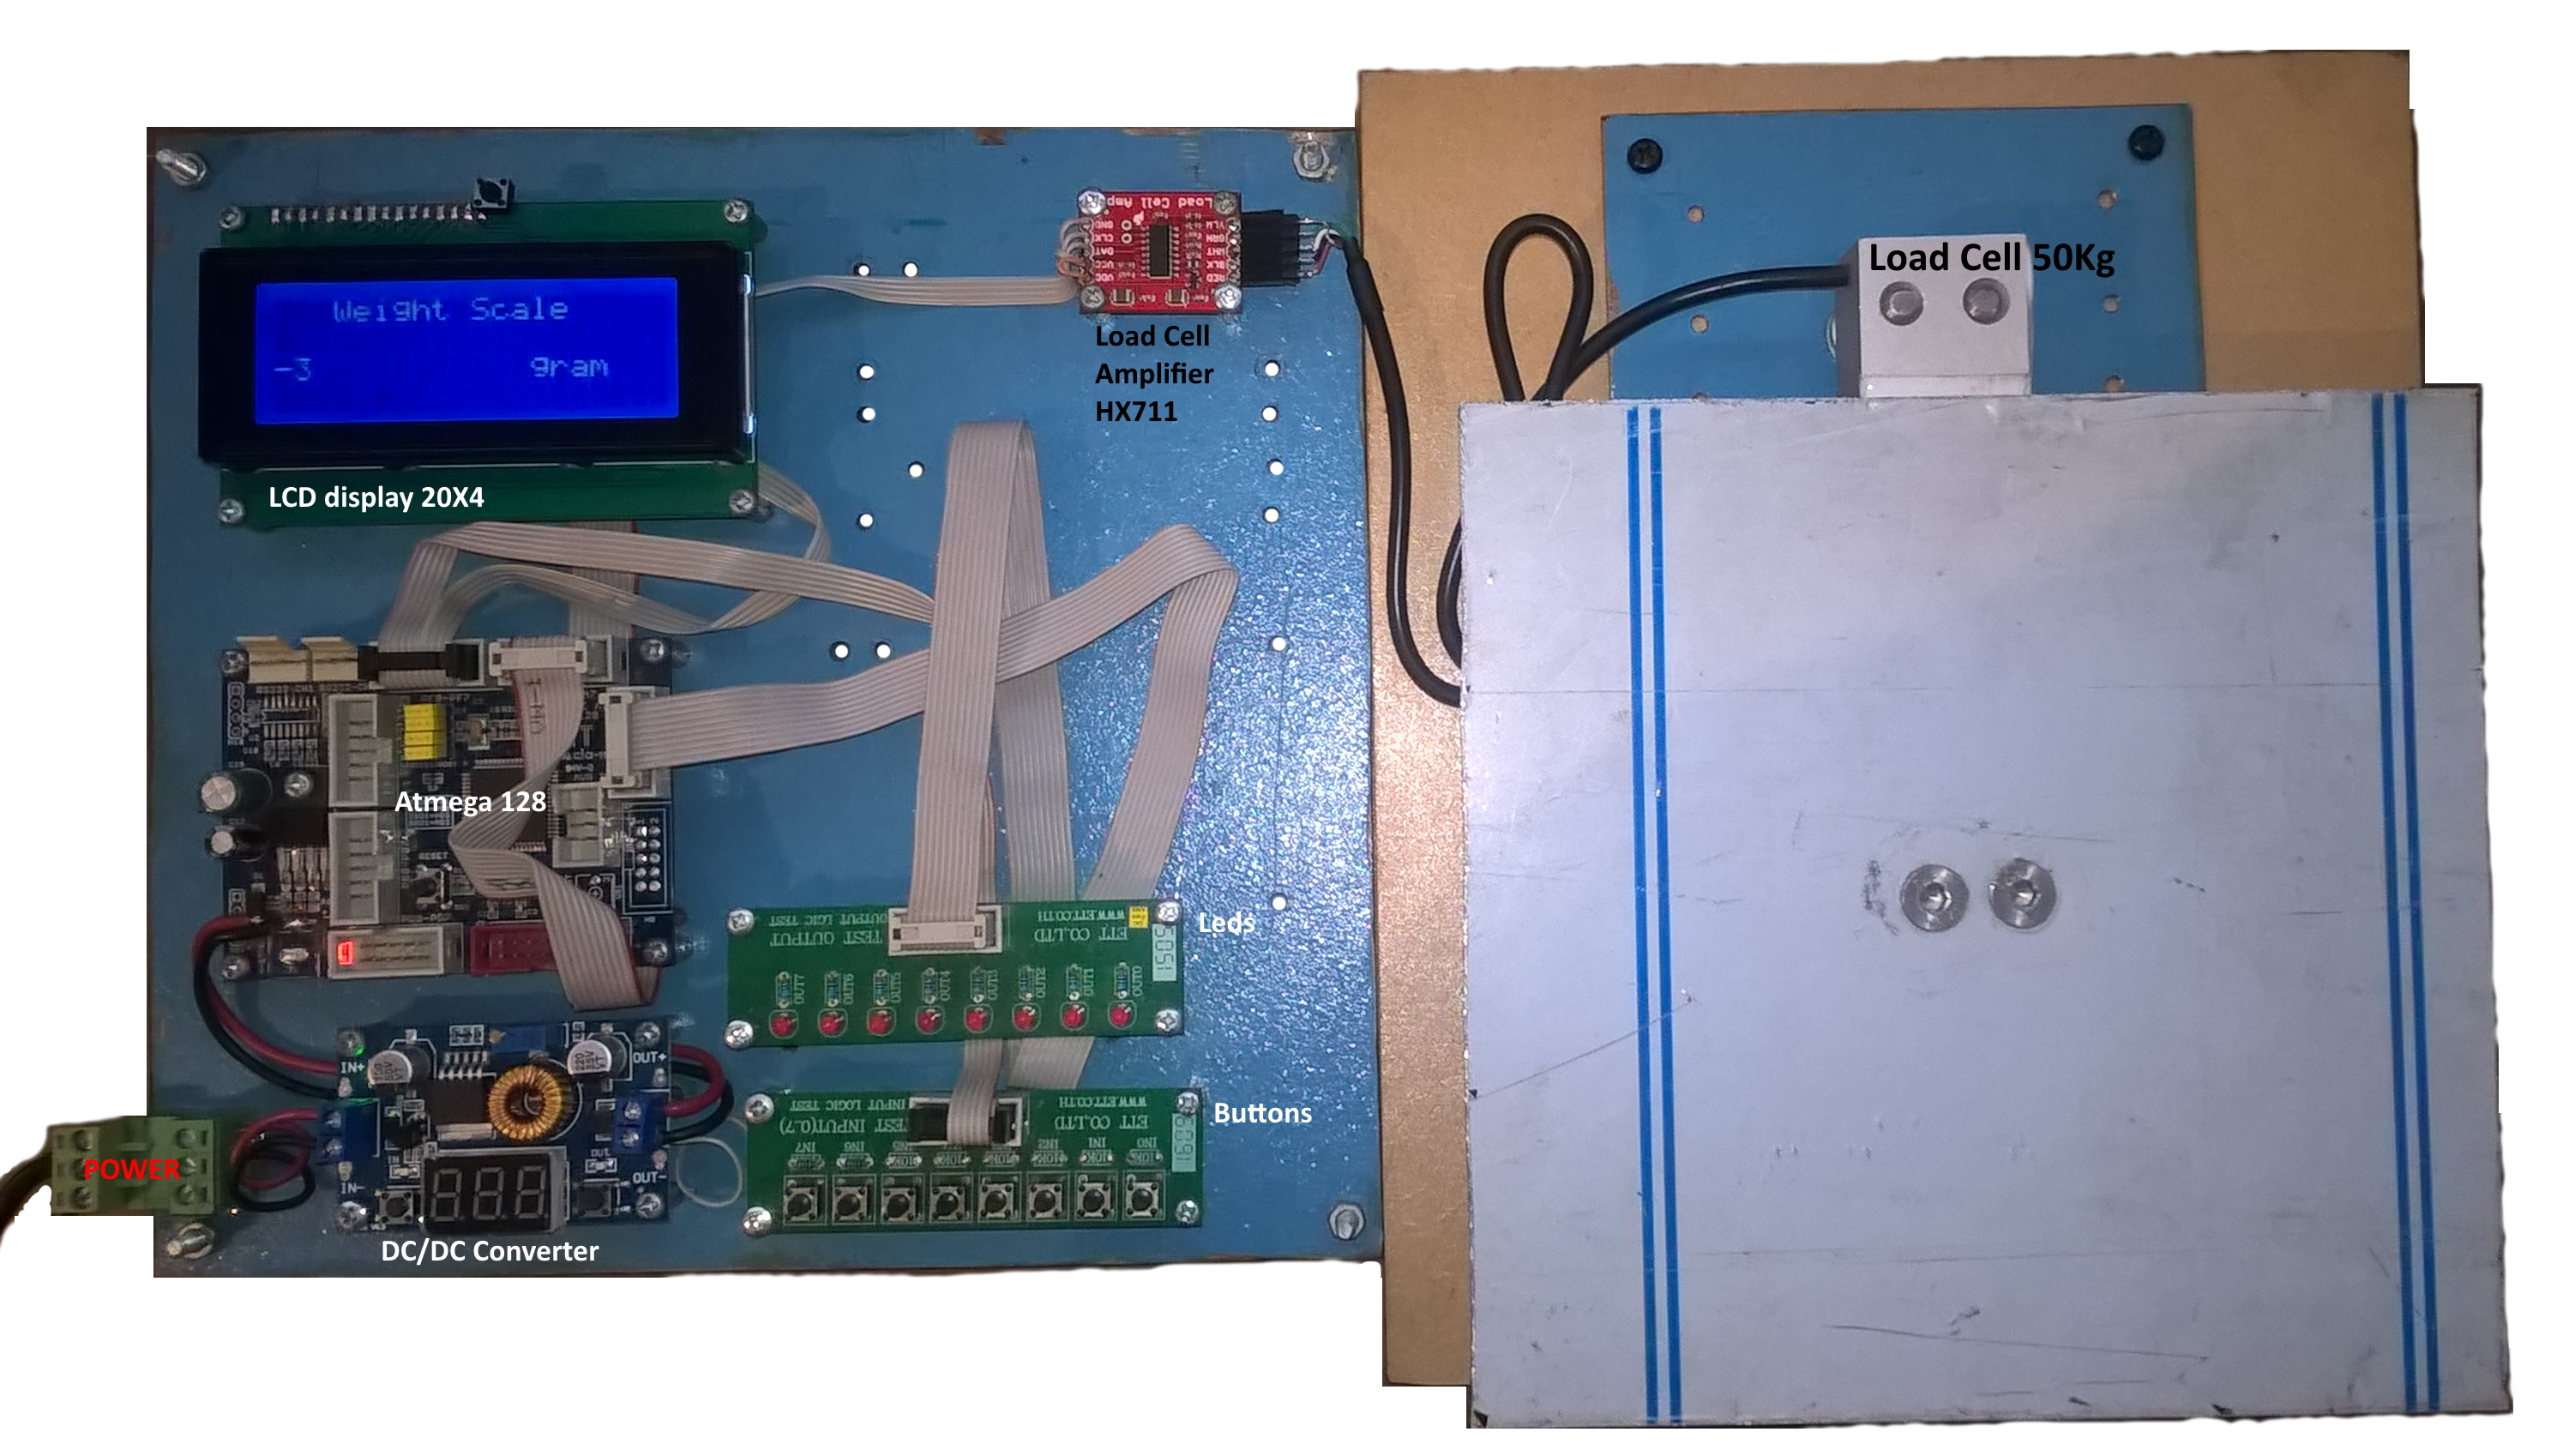
\includegraphics[scale=0.12]{./image/PESTA/kit/Kit_Desenvolvimento_2.jpg}
	\caption{Kit de Desenvolvimento}
	\label{Kit_Desenvolvimento_2}
\end{figure}
a seguir a \textit{figura} \ref{Block_diagram_1} representado os elementos em diagrama de blocos.
\begin{figure}[H]
	\centering
	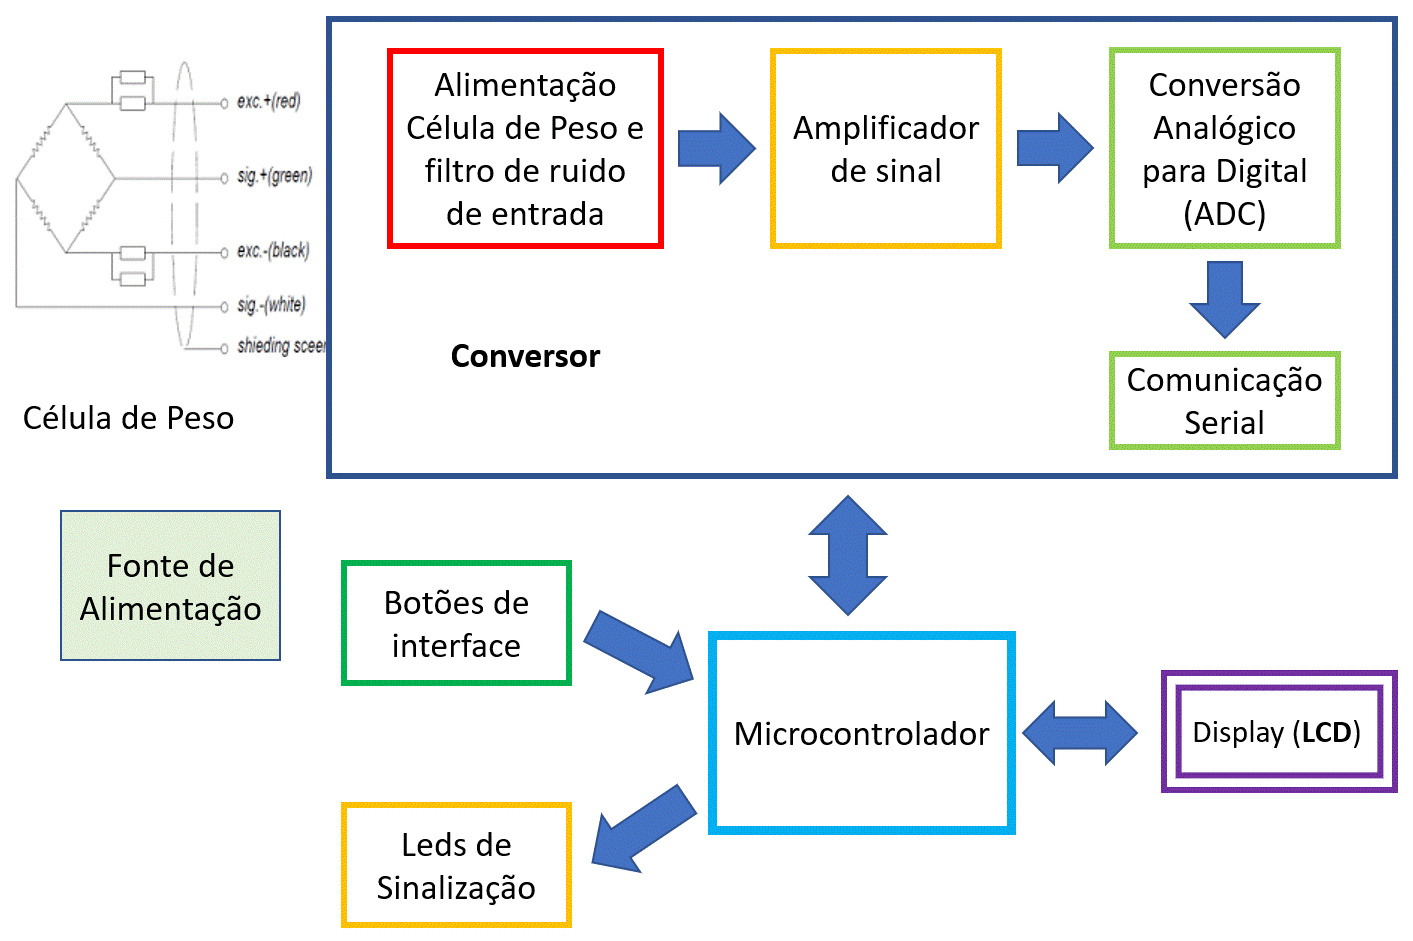
\includegraphics[scale=0.27]{./image/PESTA/Diagrama/Diagrama_bloco_3.jpg}
	\caption{Diagrama Blocos}
	\label{Block_diagram_1}
\end{figure}
\section{sensor}
Para medir a massa recorreu-se a uma \textbf{célula de peso} que determina a pressão exercida por um dado objeto, neste caso é um bloco de alumínio como indicado na \textit{figura} \ref{Load_Cell_1}, para isso ser possível este utiliza sensores Piezoresistivos numa montagem em ponte \textit{wheatstone} sobre essa superfície em locais determinados.
\\
\begin{figure}[H]
	\captionsetup{justification=raggedright,singlelinecheck=false}
	\flushleft
	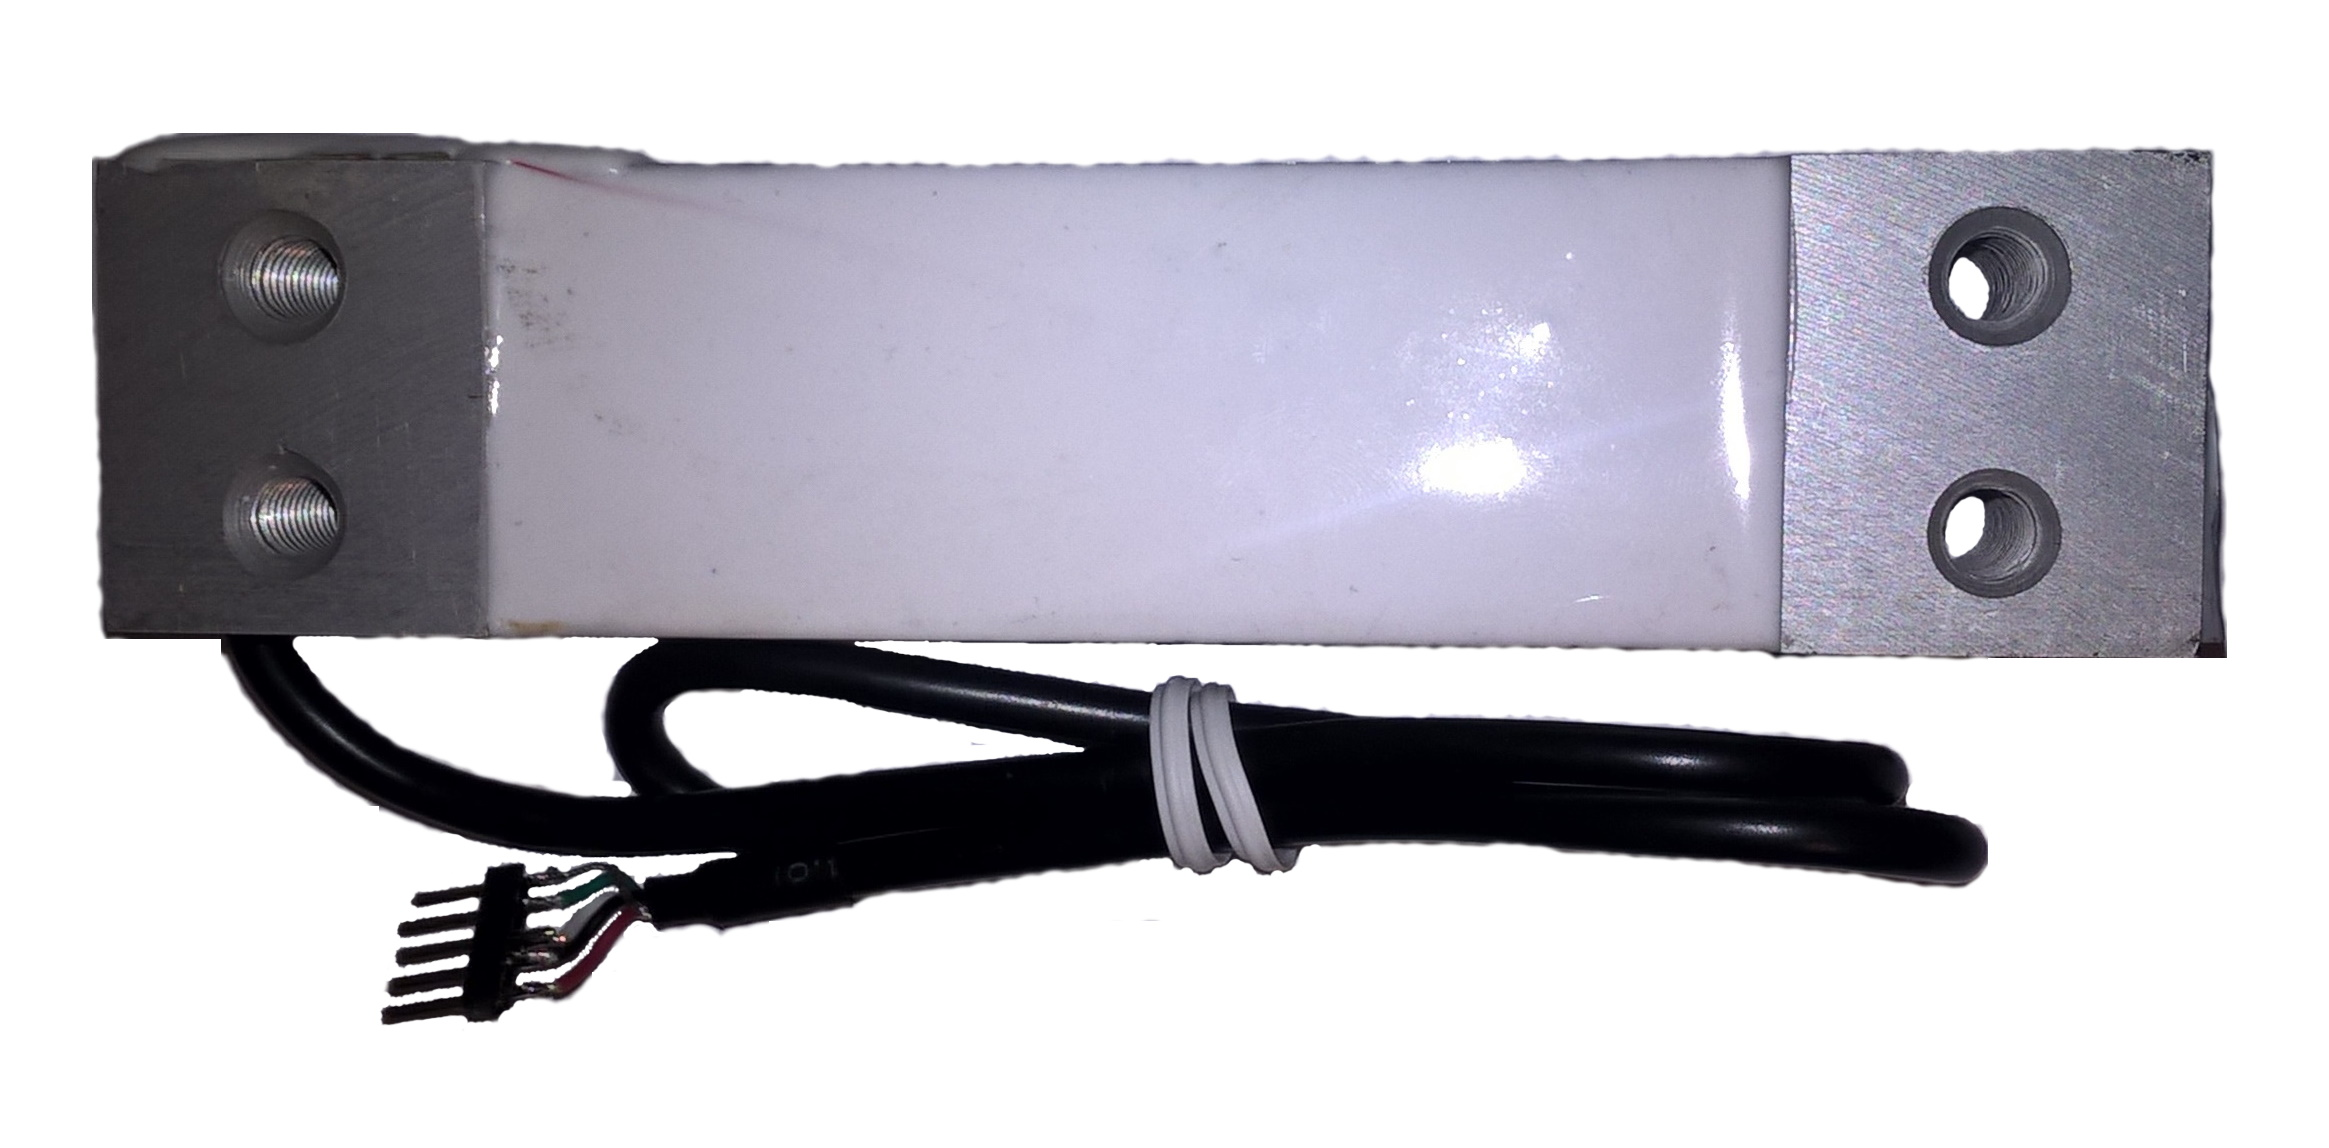
\includegraphics[scale=0.15]{./image/PESTA/material/Load_Cell_1.jpg}
	\caption{Célula de Carga 50Kg}
	\label{Load_Cell_1}
\end{figure}
\figurespace{.5}
Piezoresistividade deriva seu nome da palavra grega \textit{piezin}, que significa "pressionar". É um efeito exibido por vários materiais que exibem uma mudança na resistividade devido a uma pressão aplicada. O efeito foi descoberto pela primeira vez por Lord Kelvin em \textcolor{blue}{1856}, que notou que a resistência dos fios de cobre e ferro aumentava quando em tensão. Ele também observou que os fios de ferro apresentavam uma alteração maior na resistência do que os de cobre. A primeira aplicação do efeito piezoresistivo não apareceu até a década de \textcolor{blue}{1930}, cerca de \textcolor{blue}{75} anos após a descoberta de Lord Kelvin. Em vez de usar fios de metal, esses assim chamados medidores de tensão são geralmente feitos de uma folha de metal fina montada em uma película de suporte, que pode ser colada em uma superfície. O sensor de fita de metal típico é representado na \textit{figura} \ref{strain_gauge_1} \cite{book-9}.
\\
\\
\begin{minipage}[!b]{.5\linewidth}
	\begin{figure}[H]
		\captionsetup{justification=raggedright,singlelinecheck=false}
		\flushleft
		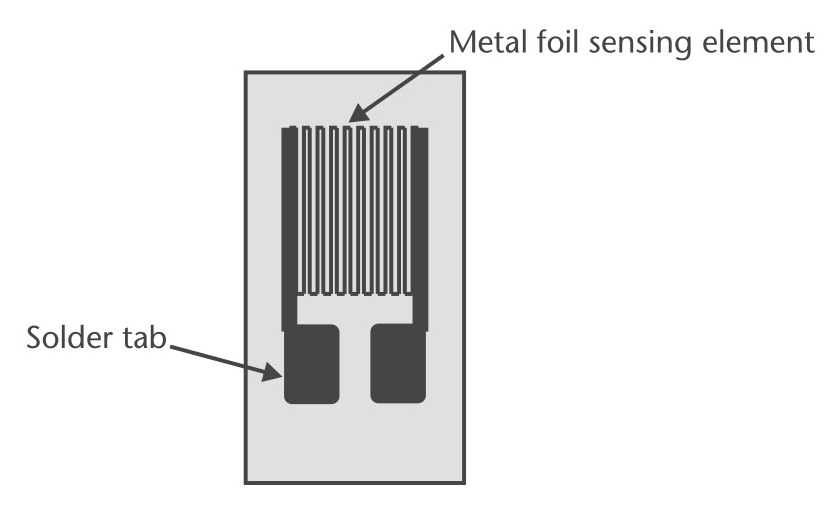
\includegraphics[height=5cm]{./image/PESTA/general/strain_gauge_1.jpg}
		\caption{Fita metálica \textit{strain gauge} \cite{book-9}}
		\label{strain_gauge_1}
	\end{figure}
\end{minipage}
\begin{minipage}[!b]{.5\linewidth}
	\begin{figure}[H]
		\captionsetup{justification=raggedright,singlelinecheck=false}
		\flushleft
		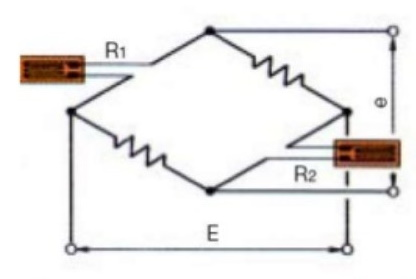
\includegraphics[height=5cm]{./image/PESTA/schematic/Wheatstone_2.jpg}
		\qquad \caption{Ponte \textit{Wheatstone}}
		\label{wheatstone_2}
	\end{figure}
\end{minipage}
\minipagespace{.5}
\begin{minipage}[!b]{.4\linewidth}
	\begin{figure}[H]
		\captionsetup{justification=raggedright,singlelinecheck=false}
		\flushleft
		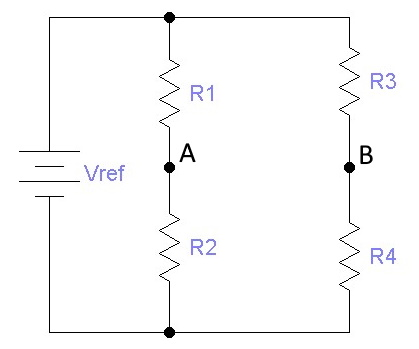
\includegraphics[height=5cm]{./image/PESTA/schematic/Wheatstone_1.jpg}
		\caption{\textit{Wheatstone} por resistências \cite{book-10}}
		\label{wheatstone_1}
	\end{figure}
\end{minipage}
\begin{minipage}[!b]{.6\linewidth}
	\begin{align}
		\label{eq:wheatstone}
		&V_A =  \frac{R_2}{R_1 + R_2} \; V_{ref} \; V_B=\frac{R_4}{R_3 + R_4} \; V_{ref} \\
		&V_{AB} =  V_A - V_B = e \\
		&V_{AB}= \left(\frac{R_2}{R_1 + R_2} - \frac{R_4}{R_3 + R_4}\right) \; Vref \\
		&e = \frac{R_2 R_3 - R_4 R_1}{(R_1 + R_2)(R_3 + R_4)} \; Vref
	\end{align}
	\minipagespace{.1}
\end{minipage}
\minipagespace{.5}
Normalmente nestas aplicações só é usados um sensor ou dois sensores em que estão nos extremos opostos  ou ligados ao mesmo ponto da alimentação, só em casos muito raros são utilizados os quatro sensores na qual a sensibilidade é máxima. E como é óbvio se o valor das quatro resistências são iguais $V_{AB}$ na saída é nula, e quando se utiliza apenas dois sensores a sensibilidade do sistema é intermédia.
\newpage
A montagem da mesa de medição \textit{figura} \ref{Prato},
\minipagespace{5}
\begin{minipage}[!b]{\linewidth}
	\begin{figure}[H]
		\centering
		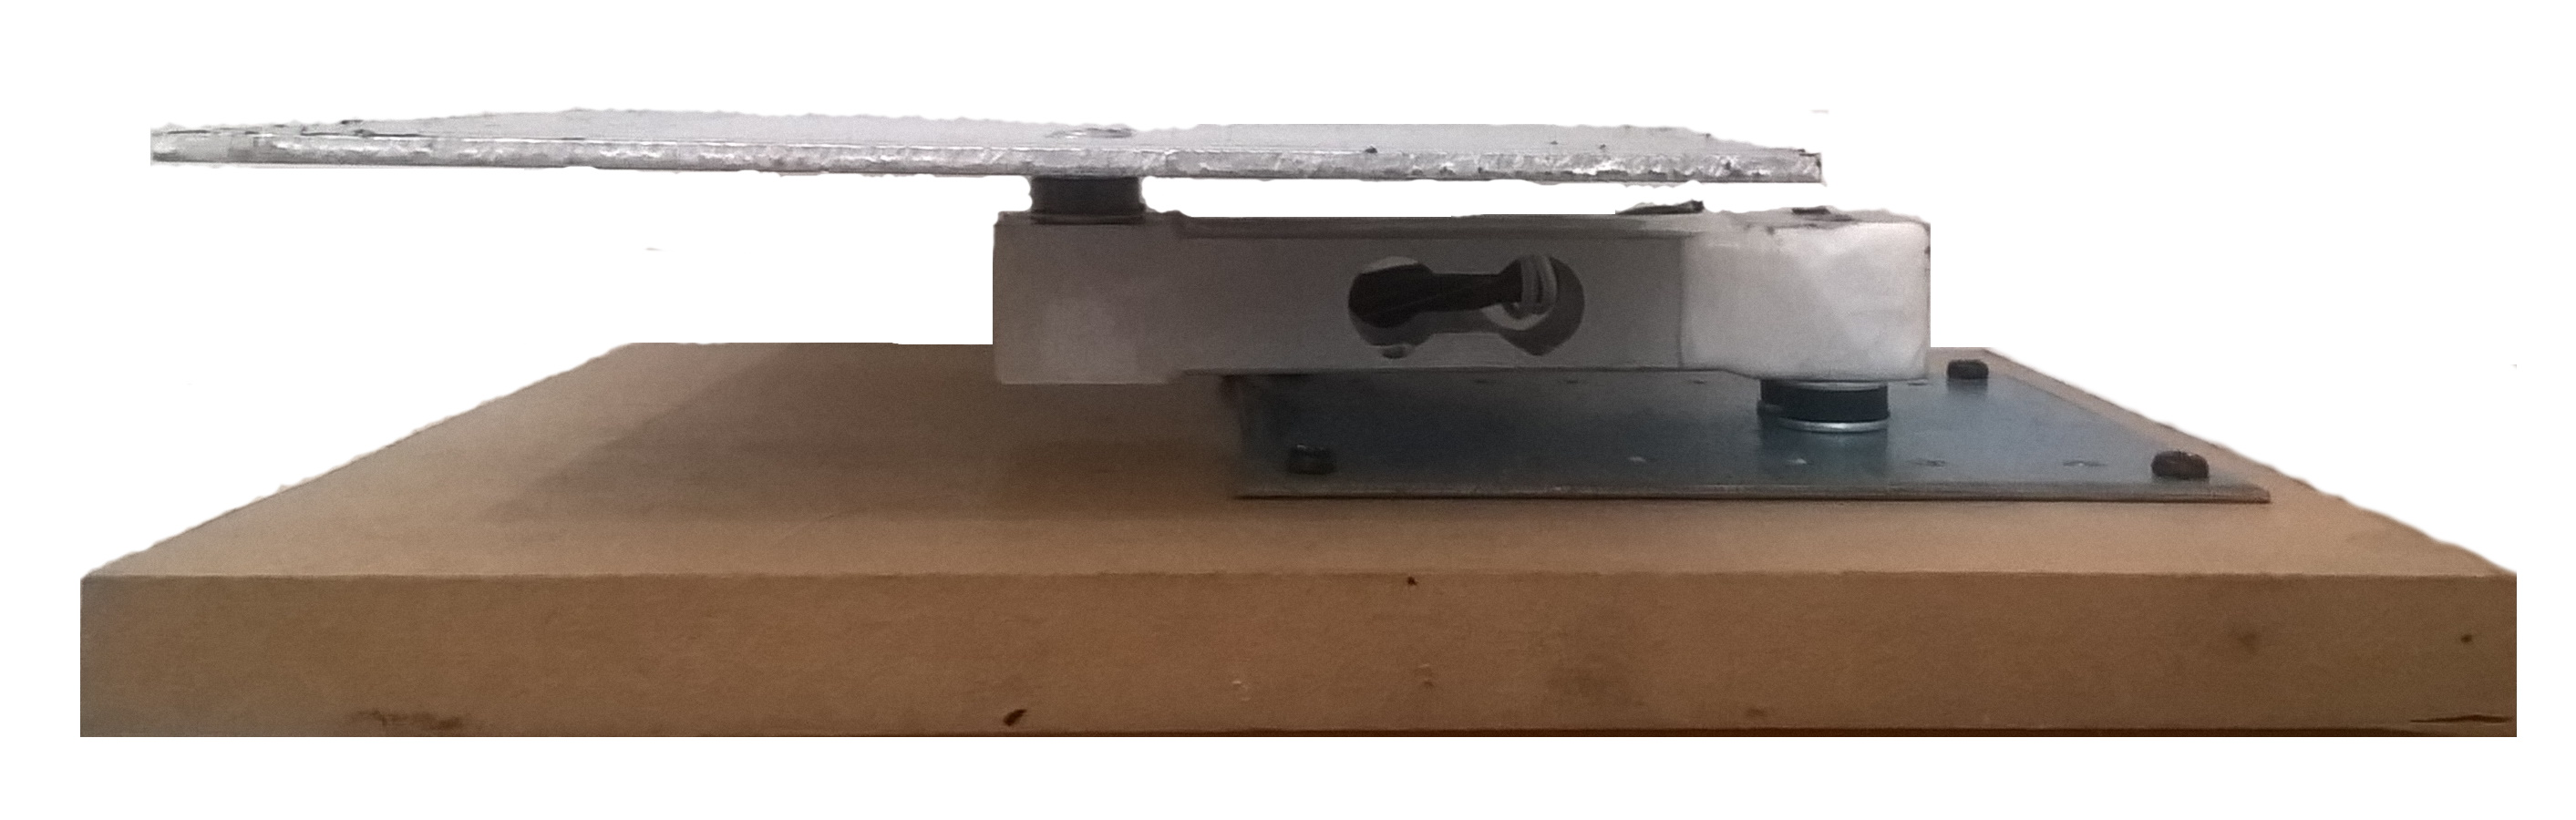
\includegraphics[scale=0.16]{./image/PESTA/material/Prato.jpg}
		\caption{Prato}
		\label{Prato}
	\end{figure}
\end{minipage}
\newpage
\section{Amplificador de sinal}
A amplificação é geralmente um requisito fundamental, pois a maioria dos sensores tende a produzir níveis de sinal significativamente mais baixos do que aqueles usados no processador digital. Sensores resistivos podem precisar de um amplificador de carga. Se possível, é vantajoso ter o ganho o mais próximo possível do elemento sensor. Em situações onde um alto ganho é necessário, muitas vezes pode haver implicações para lidar 
com quaisquer efeitos adversos, como o ruído, também em termos de \textit{layout} do \textit{chip}, os transitórios agudos associados aos sinais digitais precisam ser mantidos bem longe dos circuitos analógicos \textit{front-end}. \cite{book-9}
\\
\\
A ligação destes componentes é intuitivo e fácil de se perceber, o que é complexo neste trabalho é a interligação destes equipamentos com o micro-controlador por meio de \textit{software} e criar o \textit{driver} de comunicação para a placa do amplificador de sinal, já que o protocolo de comunicação é proprietário.
\\
\\
\begin{figure}[H]
	\captionsetup{justification=raggedright,singlelinecheck=false}
	\centering
	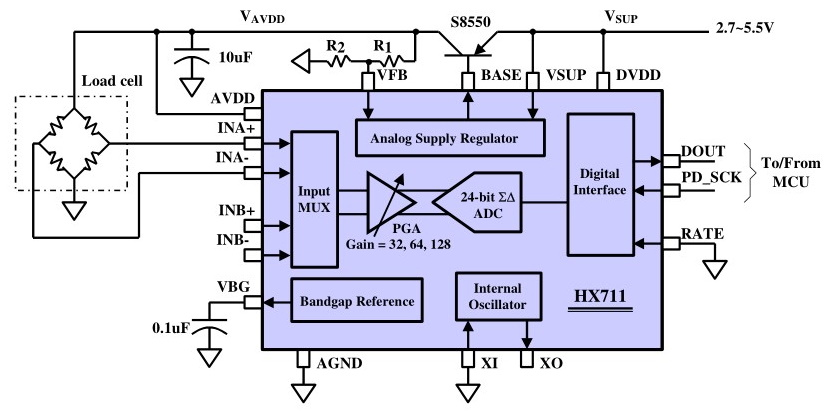
\includegraphics[scale=0.35]{./image/PESTA/schematic/HX711_Schematic_1.jpg}
	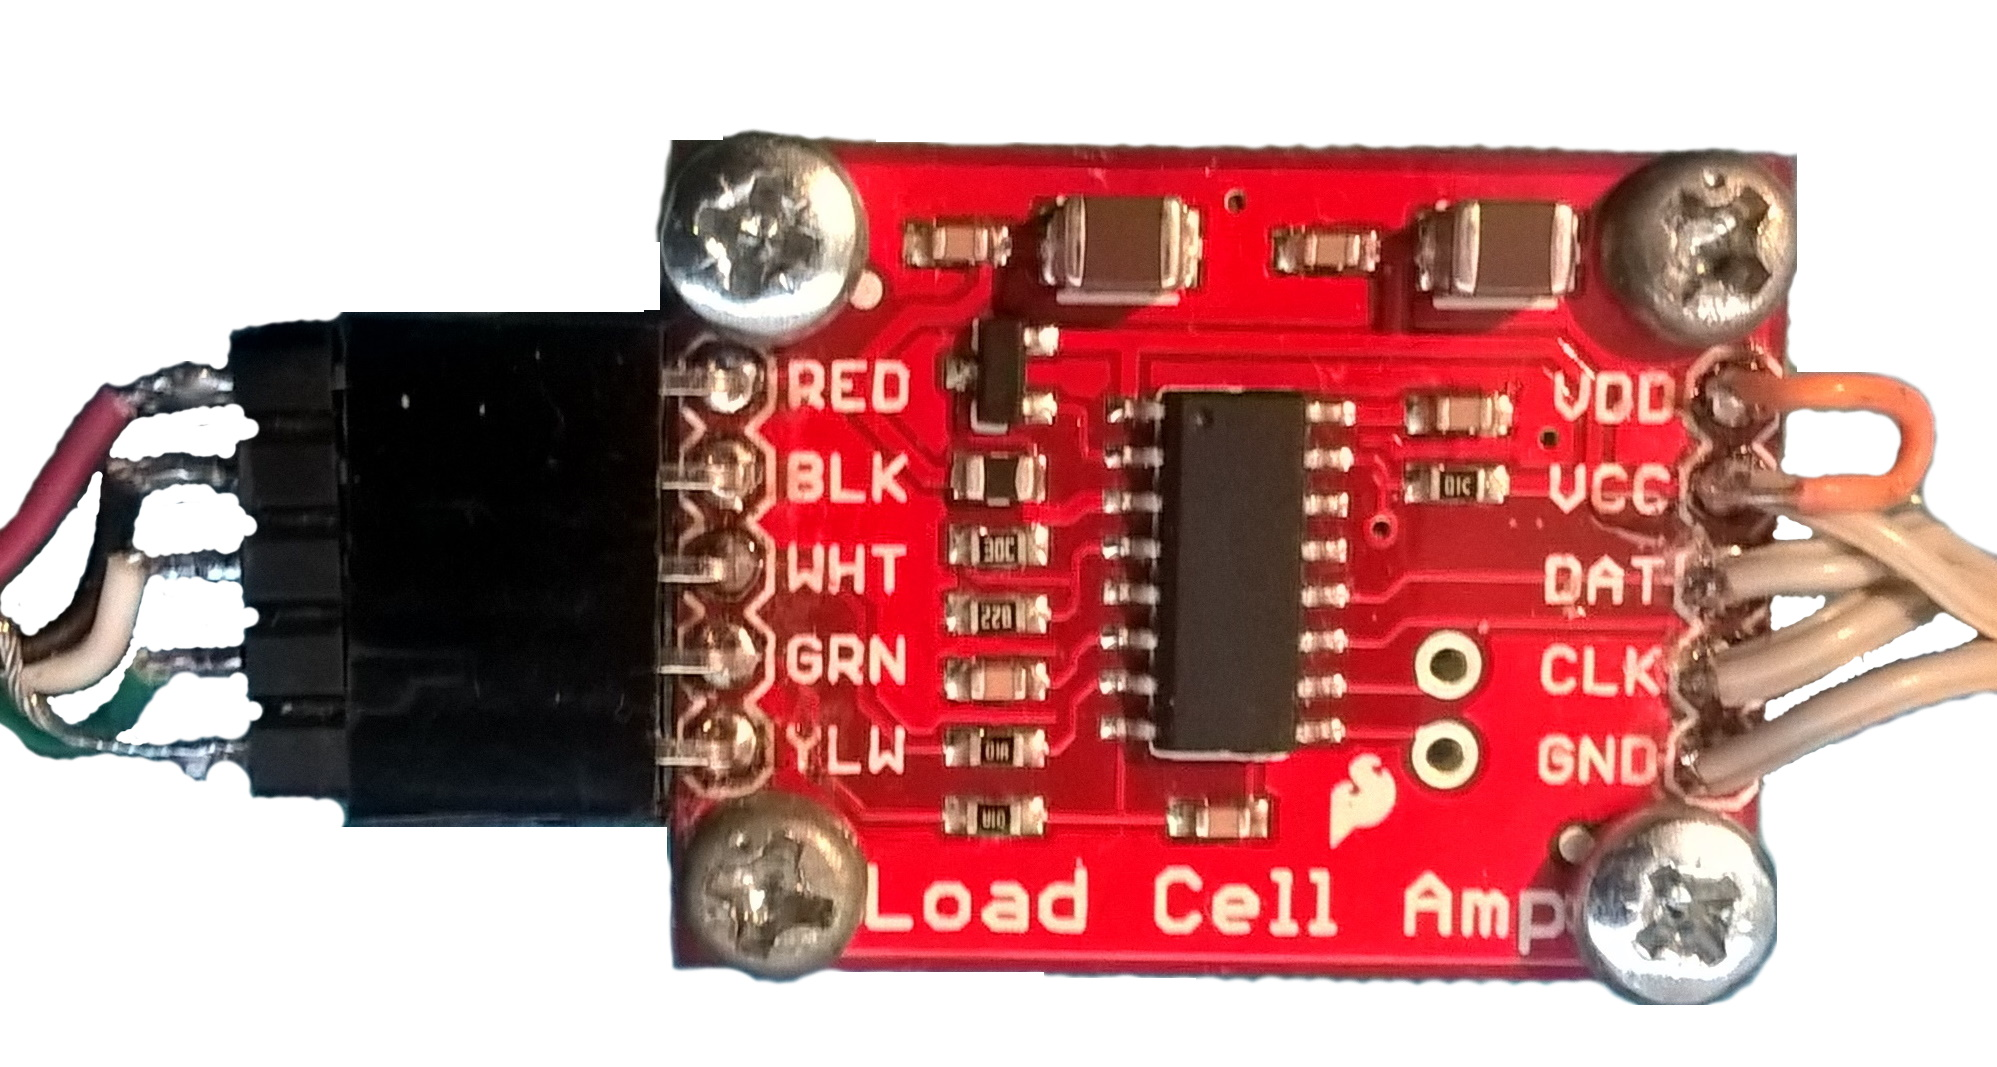
\includegraphics[scale=0.1]{./image/PESTA/material/HX711_board_1.jpg}
	\caption{Amplificador de Sinal [HX711]}
	\label{HX711_Schematic_1}
\end{figure}
\figurespace{.5}
A placa \textit{Load Cell Amplifier }pode ser programada fisicamente para determinar o numero de amostras por segundo a ser transmitido, tem opção de \textcolor{blue}{10} amostras por segundo e \textcolor{blue}{80} amostras, neste projeto optei pela segunda opção que necessita alteração na placa de circuito de impresso, isto é, abrir o \textit{jumper} respetivo de configuração.
\\
\\
\begin{table}[H]
	\centering
	\caption{Terminais HX711 ({\tiny \scriptsize{top view}})}
	\begin{tabular}{||L{1cm} C{3cm} | p{3cm}  C{2cm}||}
		\hline
		\multicolumn{2}{||c|}{MCU} & \multicolumn{2}{|c||}{\textit{Célula de peso}}\\ [1ex]
		\hline
		1 & GND & EARTH (GND) & YLW \\ 
		2 & CLK & INPA & GRN \\
		3 & DATA & INNA & WHT \\
		4 & VCC &  GND & BLK \\
		5 & VDD & $V_{ADC}$ & RED \\ [1ex]
		\hline
	\end{tabular}	
	\label{HX711_connection}
\end{table}
\tablespace{.5}
A conversão de informação é a transição entre o sinal continuo da vida real para um sinal discreto associado ao mundo digital, tipicamente esta etapa consiste na conversão analógica para digital.
\\
O processamento digital pode consistir de rotinas para compensar os desvios por linearização, compensação da sensibilidade e \textit{offset}, ou podem ser técnicas mais sofisticadas como reconhecimento de padrões (tais como redes neuronais) para equipamentos de sensores vetoriais.\cite{book-9}
\\
A comunicação trata de cuidar das rotinas necessárias para transferir e receber a informação e sinais de controle para a linha de comunicação com o sensor, e o processador que toma lugar como componente central tratando a informação, guardar os dados e fazer rotinas tais como de calibração, teste e controlo de ganho da amplificação. \cite{book-9}
\\
\\
\begin{figure}[H]
	\centering
	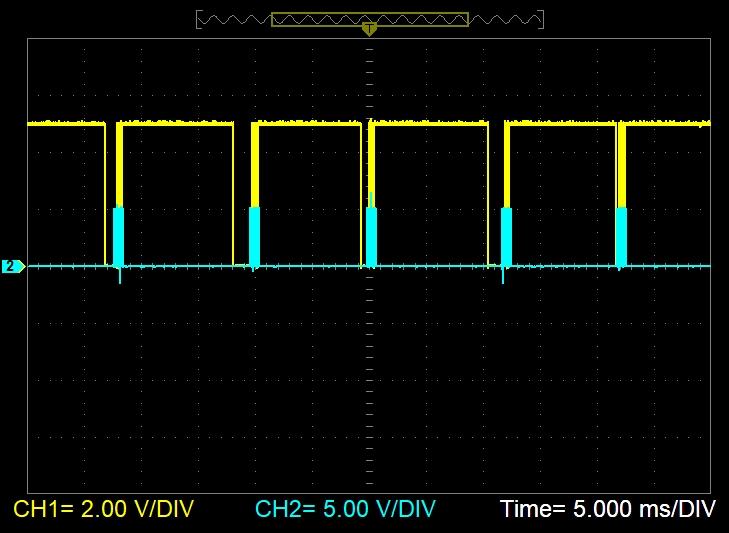
\includegraphics[scale=0.55]{./image/PESTA/graph/80SPS64GAIN/SPS_80.JPG}
	\caption{Amostras}
	\label{SPS_64}
\end{figure}
\figurespace{.5}
A livraria (\textit{driver}) criada recorre a interrupções periódicas quando o sinal de \textit{data} vai para a massa, indicando assim que tem um pacote de leitura pronto a ser transmitido.
\\
\\
\begin{minipage}[!b]{.40\linewidth}
	\begin{table}[H]
		\captionsetup{justification=raggedright,singlelinecheck=false}
		\caption{Configuração Ganho}
		\begin{tabular}{ | c | c | c |  }
			\hline
			\makecell[c]{PD\_SCK \\ Impulsos} & Entrada  & Ganho \\
			\hline
			\hline
			25 & \textbf{A} & 128 \\
			\hline
			26 & \textbf{B} & 32 \\
			\hline
			27 & \textbf{A} & 64 \\
			\hline
		\end{tabular}
		\label{Gain_Selection}
	\end{table}
	\tablespace{2}
\end{minipage}
\begin{minipage}[l]{.6\linewidth}
	\vspace{.3cm}
	Como indicado abaixo no gráfico em que a linha \textcolor{yellow}{amarela} é a informação e a linha \textcolor{BlueGreen}{azul} o respetivo \textit{clock} que é gerado pelas interrupções do micro-controlador fazendo \textit{shift} dos \textcolor{blue}{24} bits, que depois no fim transmite para o amplificador o ganho de amplificação a ser usado pelo numero excedente de \textit{clock cycles}, em que nesta demonstração \textit{figura} \ref{Gain_128_example} é \textcolor{blue}{um}, e corresponde a ganho de \textcolor{blue}{128}, respeitando a \textit{tabela} \ref{Gain_Selection},  e a sequir o exemplo da \textit{figura} \ref{Gain_64_example} com o ganho de \textcolor{blue}{64}, pois tem \textcolor{blue}{três} impulsos excedentes.
	\\
\end{minipage}
\minipagespace{.5}
\begin{minipage}[!b]{.5\linewidth}
	\begin{figure}[H]
		\captionsetup{justification=raggedright,singlelinecheck=false}
		\flushleft
		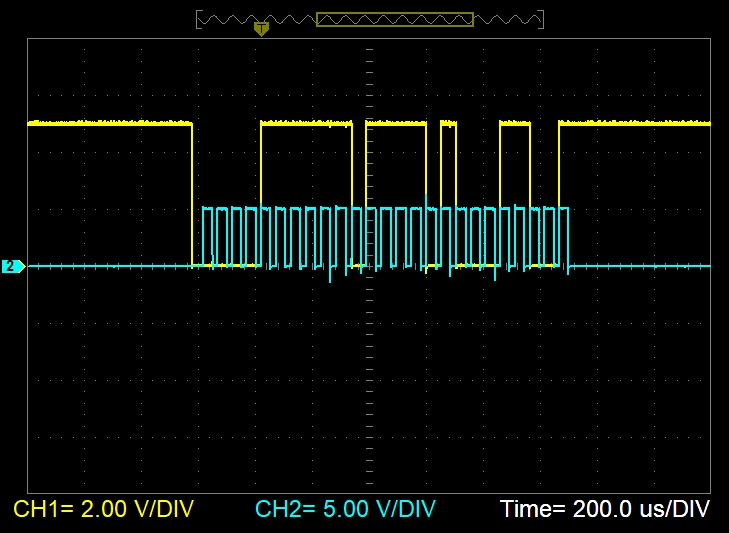
\includegraphics[scale=0.25]{./image/PESTA/graph/80SPS128GAIN/Gain_128_example.JPG}
		\caption{Ganho de 128}
		\label{Gain_128_example}
	\end{figure}
\end{minipage}
\hspace{1cm}
\begin{minipage}[!b]{.5\linewidth}
	\begin{figure}[H]
		\captionsetup{justification=raggedright,singlelinecheck=false}
		\flushleft
		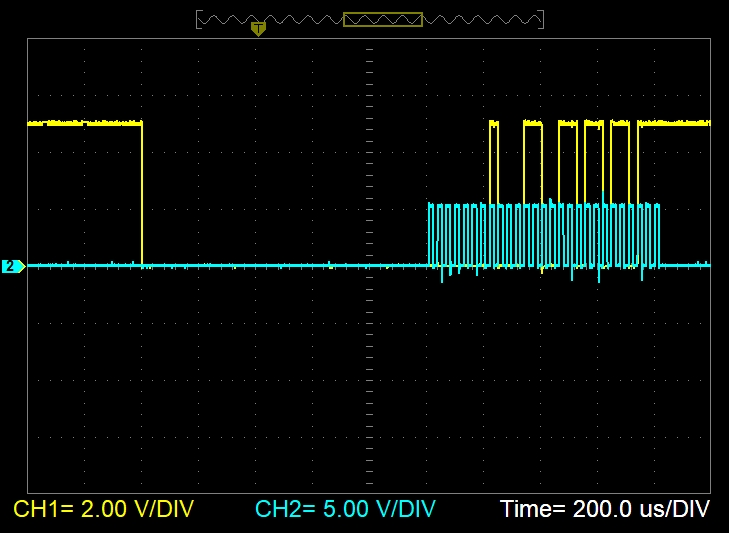
\includegraphics[scale=0.25]{./image/PESTA/graph/80SPS64GAIN/Gain_64_example.JPG}
		\caption{Ganho de 64}
		\label{Gain_64_example}
	\end{figure}
\end{minipage}
\minipagespace{.5}
Para obter este resultado a livraria driver para o \textit{Load Cell Amplifier} teve de ter em consideração que o micro-controlador é de \textcolor{blue}{8} bits, porque o pacote de informação consiste de \textcolor{blue}{24} \textit{bits} e em que é transmitido primeiro o \ac{msb}.
\\
\\
\\
O código que executa esta rotina é demonstrado na \textit{lista} \ref{HX711-read-raw} que é chamada pelas interrupções periódicas e só é ativa quando a função na \textit{lista} \ref{Main-While-case-1} \textbf{hx.query(\&hx)} é verdadeira.
\\
{ \tiny
	\lstinputlisting[language=C, caption={função de chamada \textbf{hx.query(\&hx)}}, captionpos=b, label=Main-While-case-1]{./input/code/hx_query.c}
}
\newpage
{ \tiny
	\lstinputlisting[language=C, caption=HX711\_read\_raw, captionpos=b, label=HX711-read-raw]{./input/code/HX711_read_raw.c}
}
\listingspace{.1}
Após obter um numero determinado de valores discretos é calculado sua média
\begin{equation}
	\label{eq:Mean}
	\overline{x}  =  \frac{1}{n}\sum_{i=1}^n x_i
\end{equation}
para ser tratado e deduzido o valor correspondente da massa.
\newpage
\section{Display LCD}
O \ac{lcd} utilizado é de 4x20, isto é, quatro linhas de vinte caracteres cada, é o interface humano principal, e durante o projeto uma ferramenta extremamente útil também para fazer \textit{debug} e executar testes no código.
\\
\\
Uma livraria na qual já tinha feito para outros projetos serviu para aplicar neste, poupando bastante tempo, revelando a importância de documentar os conhecimentos adquiridos. A livraria ou se preferem \textit{driver} esta \textit{anexado}.
%[\ref{codigo}]
\\
\\
Abaixo esta uma tabela \ref{LCD_connections} com as respetivas ligações.
\tablespace{.2}
\begin{table}[H]
	\centering
	\caption{Conexões \textbf{LCD}}
	\begin{tabular}{||p{1cm} p{2cm} p{4cm} | p{1cm}||} 
		\hline
		\multicolumn{3}{||c|}{\textbf{LCD Pin}} & \multicolumn{1}{|c||}{\textbf{MCU Pin}}\\ [1ex]
		\hline
		1 & VSS & GND & \\
		2 & VCC & +5V & \\
		3 & VEE & \textit{Contrast Control} & \\
		4 & RS & \textit{Register Select} & Pin 0 \\
		5 & RW & \textit{Read/Write} & Pin 1 \\
		6 & E & \textit{Enable} & Pin 2 \\
		7 & Do & \textit{Data Pin 0} & \\
		8 & D1 & \textit{Data Pin 1} & \\
		9 & D2 & \textit{Data Pin 2} & \\
		10 & D3 & \textit{Data Pin 3} & \\
		11 & D4 & \textit{Data Pin 4} & Pin 4 \\
		12 & D5 & \textit{Data Pin 5} & Pin 5 \\
		13 & D6 & \textit{Data Pin 6} & Pin 6 \\
		14 & D7 & \textit{Data Pin 7} & Pin 7 \\
		15 & LED+ & \textit{Led +5V} &  \\
		16 & LED- & \textit{Led Ground} & \\
		\multicolumn{3}{||c|}{\textit{Reboot} LCD} & \multicolumn{1}{|l||}{Pin 3}\\ [1ex]
		\hline
	\end{tabular}	
	\label{LCD_connections}
\end{table}
\begin{figure}[H]
	\centering
	%%\captionsetup{justification=raggedright,singlelinecheck=false}
	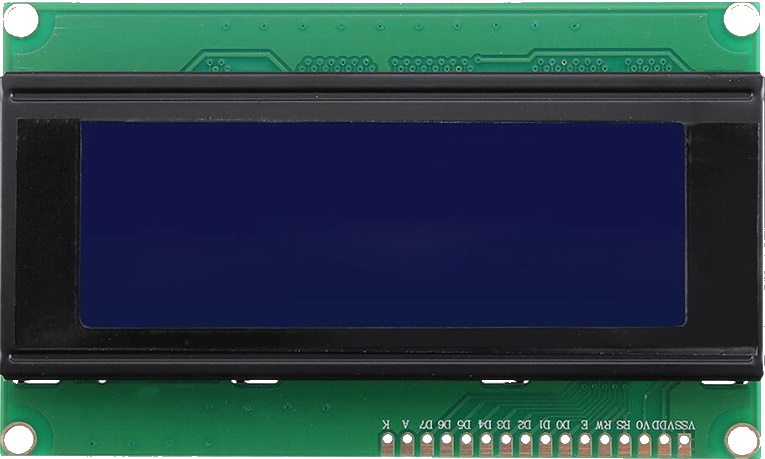
\includegraphics[scale=.5]{./image/PESTA/material/4x20_LCD.jpg}
	\caption{LCD}
	\label{4x20_LCD}
\end{figure}
\newpage
\section{Micro-controlador}
Os micro-controladores da \textbf{Atmel} de 8 e 32 bits são baseados na arquitetura avançada de \textbf{Harvard} na qual esta concebido para baixos consumos e performance.
\\
\\
Este tipo de arquitetura tem dois  \textit{busses} (barramentos) um dedicado a leitura das instruções a executar e outra para escrita e leitura de \textit{data} (informação ou dados), isto assegura que uma nova instrução pode ser executada em cada ciclo de relógio, na qual elimina estados de espera quando não ha instruções prontas a executar.
\\
\\
Nos microcontroladores da \textbf{AVR} os barramentos estão configurados de forma a dar prioridade ao barramento das instruções do \ac{cpu} acesso a memoria flash enquanto o barramento da CPU de dados tem prioridade de acesso a \ac{sram}.
\\
\\
O espaço de memoria de dados é dividida em três, os \ac{gpr} as \ac{sfr} ou memoria de I/O e a \textit{data} \textbf{SRAM}.
\\
\\
Os microcontroladores da \textbf{AVR} utiliza uma arquitetura de instruçõeses \ac{risc} na qual reduz a complexidade dos circuitos na codificação de cada instrução.
\\
\\
Dai que os micro-controladores que se baseiam nestes tipos de arquitetura são sinonimo de código reduzido, alta performance e baixo consumo energético.
\\
\\
\begin{figure}[H]
	\centering
	%%\captionsetup{justification=raggedright,singlelinecheck=false}
	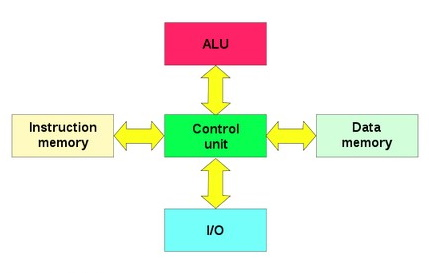
\includegraphics[scale=1]{./image/PESTA/Diagrama/Harvard_architecture.jpg}
	\caption{Harvard Architecture}
	\label{Harvard_architecture}
\end{figure}
\qquad link: \url{https://en.wikipedia.org/wiki/Harvard_architecture}
\newpage
Neste projeto apostei no Atmega 128 (\textit{figura} \ref{Atmega_128_pinagem}) por ser um dos mais poderosos \ac{mcu} da linha de 8 b\textit{bit} da Atmel, também por estar integrado já numa placa de desenvolvimento usando o sistema por fichas \ac{idc} que prefiro, ou seja, usando \textit{flatcables} para ligar os periféricos, e considero muito mais pratico do que sistema que esta na moda, tais como a linha Arduino, STMicroelectronics e a \ac{pic} por ter um interface por pinos.
\\
\\
\\
\\
\\
\begin{figure}[H]
	\centering
	%%\captionsetup{justification=raggedright,singlelinecheck=false}
	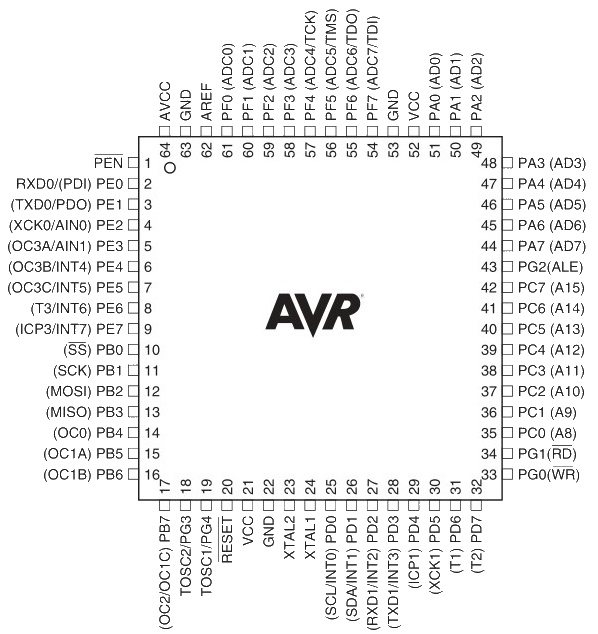
\includegraphics[scale=0.7]{./image/PESTA/material/Atmega128_1.jpg}
	\caption{Atmega 128}
	\label{Atmega_128_pinagem}
\end{figure}
\figurespace{1}
{Transparências Sistemas Digitais 2 \quad \textbf{ISEP} \quad 2008/2009 \quad \textit{link}}:
\\
\url{https://drive.google.com/file/d/1wgOGf8WwYY0OzDhRca9ypXz-iBO55YOF/view?usp=sharing}
\newpage
A características do micro-controlador ATmega 128 esta abaixo indicados na lista, os temporizadores considero o mais importante, o \ac{adc} nem vai ser usado neste projeto a alternativa é muito melhor, talvez os MCU nem deviam ter esta funcionalidade e realçar em meios de comunicação e memoria com as livrarias já disponíveis, este integrado é perfeito para esta aplicação em causa, sempre que fazemos projetos também temos de considerar os MCU de 32 \textit{bit} mas existe uma linha muito fina de apostar noutra alternativa e trabalhar com um sistema operativo devido a complexidade exigida, muito mais configurações e opções disponíveis do que um micro-controlador de 8 e 16 \textit{bit}.
\\
\\
\\
\begin{minipage}{\linewidth}
	{\Large Caracteristicas do Atmega 128 :}
	\begin{itemize}	
		\setlength\itemsep{-0.3em}
		\item Arquitectura RISC
		\item 33 instruções (a maior parte executada num único ciclo de execução)
		\item 32 x 8 registos de trabalho (arquitectura de registos)
		\item Até 16 MIPS (@16MHz) – 62.5ns / instrução
		\item 64K x 16 palavras de programa – 128K bytes FLASH
		\item 4K bytes de RAM interna
		\item 4K bytes de E2PROM de dados
		\item Ciclos de escrita / leitura – FLASH=10000, E2PROM=100000
		\item 7 Portos de IO \\
		\hspace*{.5cm}	-> 6 x 8 bits (Portos A .. F) \\
		\hspace*{.5cm}	-> 1 x 5 bits (Porto G)
		\item 2 x Timer / Counter de 8 bits
		\item 2 x Timer / Counter de 16 bits
		\item 1 x Real Time Counter ( com oscilador independente)
		\item 2 x PWM de 8 bits
		\item 6 x PWM de 16 bits
		\item ADC de 10 bits (8 canais)
		\item 2 x USART
		\item SPI
		\item TWI (I2C)
	\end{itemize}
\end{minipage}
\minipagespace{0.5}
\newpage
Para programar este microcontrolador (\textbf{Atmega 128}) foi utilizado o programador da marca da Atmel precisamente o \ac{atmel-ice} \textit{figura} \ref{Programador_1}, que para este equipamento tem disponível programação via \ac{isp} \textit{figura} \ref{ISP_6_8_10pin} e \ac{jtag}.
\minipagespace{.2}
\begin{minipage}[!b]{.5\linewidth}
	\begin{figure}[H]
		\captionsetup{justification=raggedright,singlelinecheck=false}
		\flushleft
		\includegraphics[scale=0.75]{./image/PESTA/programador/Atmel_ice.png}
		\caption{KIT ATMEL-ICE}
		\label{Programador_1}
	\end{figure}
\end{minipage}
\hspace{.5cm}
\begin{minipage}[!b]{.5\linewidth}
	\begin{figure}[H]
		\captionsetup{justification=raggedright,singlelinecheck=false}
		\flushleft
		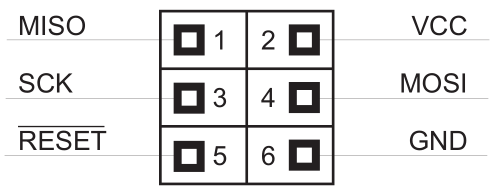
\includegraphics[scale=0.45]{./image/PESTA/programador/isp_6pin.png}
		\hspace{.3cm}
		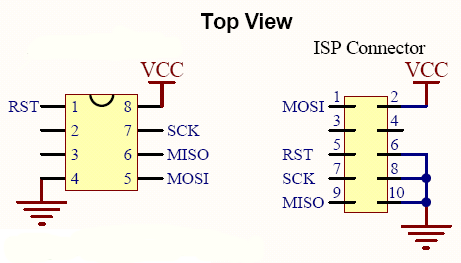
\includegraphics[scale=0.5]{./image/PESTA/programador/isp_8e10pin.png}
		\caption{Fichas \textbf{ISP}}
		\label{ISP_6_8_10pin}
	\end{figure}
\end{minipage}
\section{Fonte de Alimentação}
\begin{minipage}[!b]{.5\linewidth}
	\begin{figure}[H]
		\captionsetup{justification=raggedright,singlelinecheck=false}
		\flushleft
		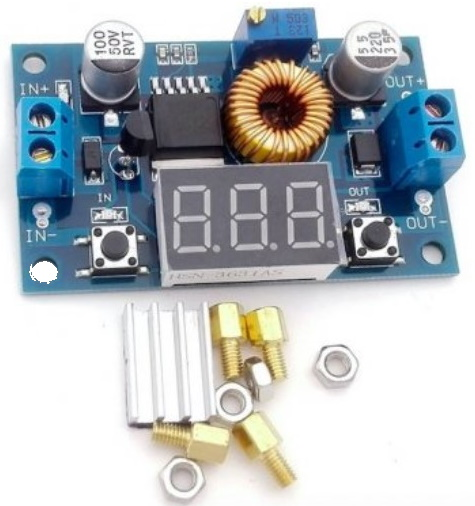
\includegraphics[scale=0.5]{./image/PESTA/material/DCDC_converter.jpg}
		\caption{\textit{Buck Converter}}
		\label{buck-converter}
	\end{figure}
	\figurespace{.1}
\end{minipage}
\begin{minipage}[!b]{.5\linewidth}
	\small
	Caracteristicas DC/DC:
	\begin{itemize}
		\setlength\itemsep{-0.5em}
		\footnotesize
		\item 5A 75W Conversor Abaixador (\textit{Step-down})
		\item Alimentação Entrada: 4 - 38VDC
		\item Tensão de saída: 1.25 - 36VDC
		\item Corrente saída: 0 - 5A
		\item Potência saída: 75W
		\item Voltímetro: 4 até 40V, erro ±0.1V
		\item \textit{Led} indicadores
		\item Frequência de operação: 180KHz
		\item Eficiência até 96 \%
		\item Proteção Térmica
		\item Limitador de Corrente
		\item Proteção contra curto circuito
		\item NOTA: Não tem proteção de inversão de polaridade
		\item L x W x H = 6.6 x 3.9 x 1.8 CM
		\item Massa: 28g
	\end{itemize}
\end{minipage}
Como a \textit{motherboard} tem um regulador de tensão de 5 Volt para aumentar a eficiência  e ter uma alimentação variável de entrada utilizo o \textit{Buck Converter} da \textit{figura} \ref{buck-converter}.
\chapter{Software}
\label{Chapter3}
O \ac{ide} utilizado neste trabalho foi o \textbf{\textit{{Microchip Studio for AVR\textsuperscript{\textregistered} and SAM Devices}}} (\textit{version: 7.0.2542}). A programação foi feita em Linguagem \textbf{C}, sua estrutura sintática esta abaixo mencionado:
\\
\\
\begin{figure}[H]
	\centering
	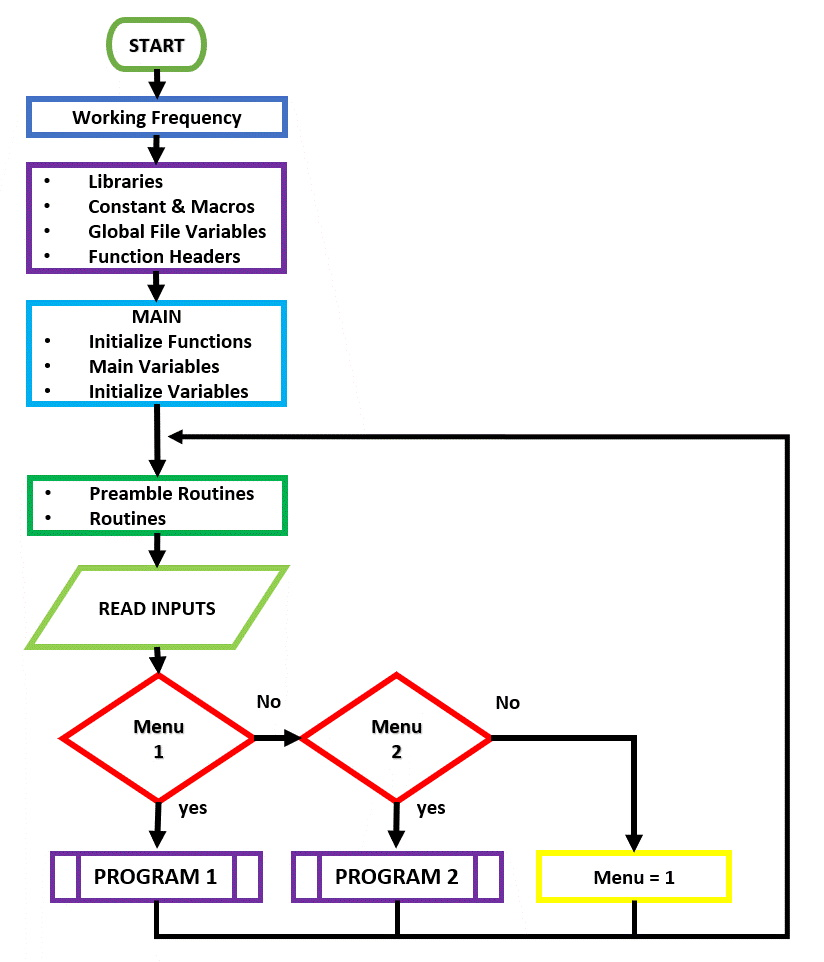
\includegraphics[scale=0.6]{./image/PESTA/flowchart/Main_Program_1.jpg}
	\caption{Estrutura do Programa (fluxograma)}
	\label{Main_Program_1}
\end{figure}
\figurespace{.5}
O \textit{PROGRAM 1} é onde corre o programa da balança, e o \textit{PROGRAM 2} usado para calibração do \textit{Gain Factor}.
\\
\\
Todos os programas sequem uma estrutura sintática recursiva usando o seguinte modelo.
\\
\\
\begin{figure}[H]
	\centering
	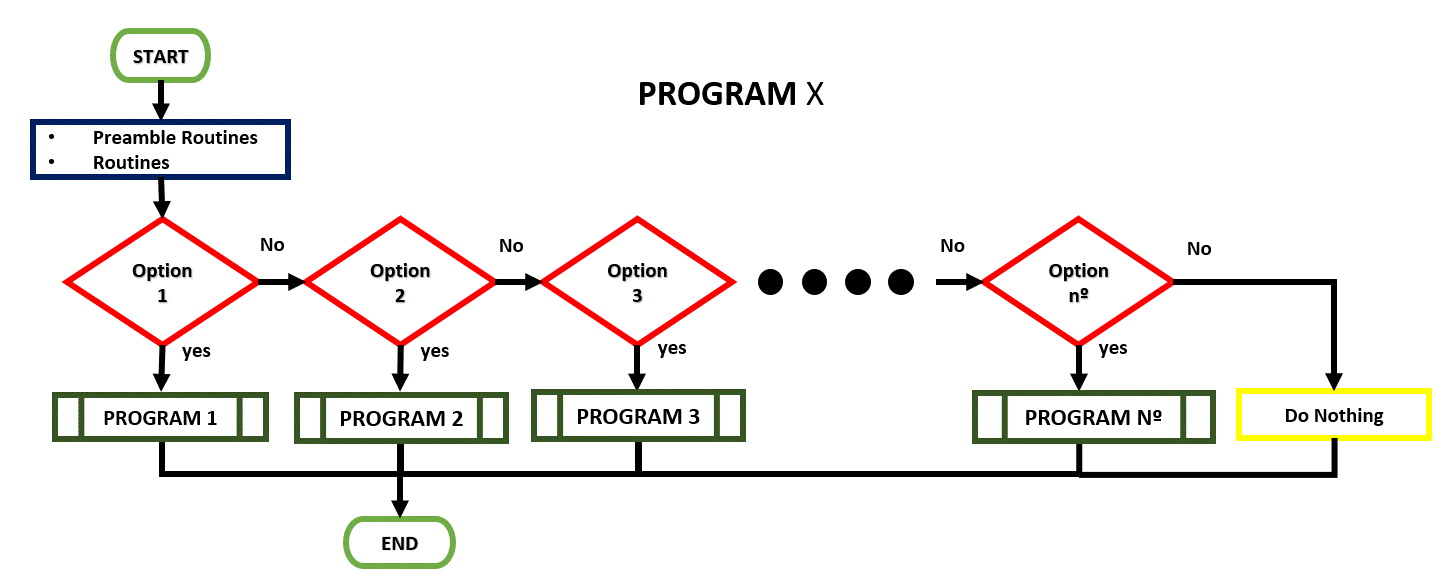
\includegraphics[scale=0.40]{./image/PESTA/flowchart/Generic_structure.jpg}
	\caption{Sintaxe Genérica dos programas (fluxograma)}
	\label{Geneic_structure}
\end{figure}
\figurespace{.5}
Duas interrupções periódicas estão sempre a correr em \textit{background}, uma para fazer o \textit{shift} dos \textit{bit´s} da conversão \textbf{ADC} feita pelo amplificador de sinal HX711 e outra interrupção periódica de segundo em segundo usado para saltar de \textit{Menu} pelos botões.
\\
\\
\begin{minipage}{\linewidth}
	\begin{minipage}{.5\linewidth}
		\begin{figure}[H]
			\centering
			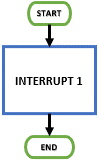
\includegraphics[scale=0.7]{./image/PESTA/flowchart/Interrupt_1.jpg}
			\caption{\textbf{ADC} conversão}
			\label{Interrupt_1}
		\end{figure}
	\end{minipage}
	\begin{minipage}{.5\linewidth}
		\begin{figure}[H]
			\centering
			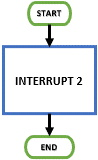
\includegraphics[scale=0.7]{./image/PESTA/flowchart/Interrupt_2.jpg}
			\caption{Saltar de \textit{Menu}}
			\label{Interrupt_2}
		\end{figure}
	\end{minipage}
\end{minipage}
\minipagespace{.5}
Consultar código para leitura das rotinas de interrupção nas folhas \textit{anexas}.
\\
\\
\begin{minipage}{.40\linewidth}
	\begin{figure}[H]
		\flushleft
		\captionsetup{justification=raggedright,singlelinecheck=false}
		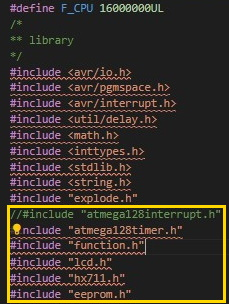
\includegraphics[scale=0.9]{./image/PESTA/Code/Livrarias.jpg}
		\caption{Livrarias}
		\label{Livrarias}
	\end{figure}
\end{minipage}
\begin{minipage}{.6\linewidth}
	Ao lado esta as livrarias usadas neste projeto, as que estão dentro da caixa amarela são as que foram criadas.
	A filosofia usada é de criar objetos que representam o hardware para o poder manipular via código. Como se pode observar foi criado uma livraria para os temporizadores, outra para as interrupções e \ac{eeprom}, depois criado livrarias para os componentes externos, isto é, o \textbf{LCD} e o integrado \textbf{HX711}. \\
	Uma abstração que torna simples executar qualquer algoritmo ou projeto, e isto só é possível depois de ultrapassar a barreira árdua e dolorosa de desenvolver as livrarias.
	\\
	\\
	\\
\end{minipage}
\minipagespace{.5}
Durante este projeto tentou-se dentro do possível sempre seguir as boas praticas de programação, como a \texttt{indentação} especifica para cada situação, e manter a estrutura de norma. Deve-se manter uma metodologia de trabalho que segue as normas assim é percetível para todos e facilita detetar \textit{bugs}, e é uma pratica que abrange todas as linguagens, por exemplo o \textbf{Python} é fundado nesse principio.
\\
\\
Quanto as interrupções é sempre um desafio, porque as tarefas tem que ser bem organizadas temporalmente para não entrar em conflitos, pretende-se assim sempre que o código corra na função \textit{main} e as interrupções algo esporádico e muito rápido, estas devem servir de \textit{flags} para executar rotinas na função \textit{main}, ou seja, servirem de \textbf{\textcolor{green}{INPUTS}}.
\newpage
\section{Validação}
%%%To validate is to justify why the choices made and alternatives that could be chosen.
As escolhas feitas estão dentro dos parâmetros da oferta disponibilizada. Apenas o conhecimento adquirido ao aprofundar o funcionamento dos componentes é o ganho mais evidente, facilitando a interpretação de situações e deteção de anomalias (\textit{troubleshooting}), derivado aos custos dos materiais serem caros.\\
\\
Apostei na marca \textbf{Atmel} devido a experiência e conhecimentos já adquiridos, se aposta-se noutra marca teria de enfrentar uma curva de aprendizagem e adaptação que no final a nível de custos beneficio seria desfavorável, pelo tempo a dispensar e de ser muito trabalhoso a refazer tudo novamente noutra arquitetura.\\
\\
O sensor usado é o mais comum nesta pratica, e escolha demonstrada, o circuito de interface é indiferente a escolha apenas é baseada na sua precisão, ou seja, é de \textcolor{blue}{24} \textit{bit} enquanto o \textbf{ADC} do \textbf{MCU} de \textcolor{blue}{10} \textit{bit}.
\\
\\
\\
\subsection{Material}
Abaixo esta indicado uma tabela dos materiais usados, assim como os preços.
\\
\\
\begin{table}[H]{
		\caption{Lista de material}
		\rowcolors{3}{blue!80!yellow!50}{blue!70!yellow!40}
		\begin{tabular}{ |p{12cm}|c|p{2cm}|  }
			\hline
			\multicolumn{3}{|c|}{Lista de Material} \\
			\hline
			Peça & Quant & Preço [uni] \\
			\hline
			Fonte de alimetação 12V 1A & 1 & \EUR{3.87} \\
			Conversor DC-DC com voltímetro & 1 & \EUR{7.75} \\
			ET BASE AVR Atmega128 Board & 1 & \EUR{23.92} \\
			Test Input Board  & 1 & \EUR{3.71} \\
			Test Output Board & 1 & \EUR{3.71} \\
			IDC Socket 10 way    & 12 & \EUR{0.31} \\
			IDC Header Straight 10 way    & 12 & \EUR{0.25} \\
			Flatcable    & ? & \EUR{?} \\
			20x4 LCD Module Blue & 1 & \EUR{12.24} \\
			SparkFun Load Cell Amplifier HX711 & 1 & \EUR{13.04}   \\
			50Kg Load Cell & 1 & \EUR{12} \\
			\hline
			& \textit{total} & \EUR{86.96} \\
			\hline
		\end{tabular}
	}
	\label{material}
\end{table}
\newpage
\subsection{Testar}
Quanto a funcionalidade no seu todo a balança tem \textcolor{blue}{quatro} botões e \textcolor{blue}{três} \textit{leds} ativados, um botão para fazer o \textit{offset} no \textcolor{green}{PORTF 0}, e dois botões com dupla função, fazer \textit{reset} para \textit{default} e incrementar, outro para entrar no menu de calibração e decrementar, o \textcolor{blue}{quarto} botão é reservado para \textit{enter} e assumir o valor introduzido na calibração.\\
\\
O botão \textcolor{green}{PORTF 3} quando premido durante \textcolor{blue}{cinco} segundos faz um \textit{reset} para configuração \textit{default} depois de o \textit{led} no \textcolor{red}{PORTC 6} piscar \textcolor{blue}{quatro} vezes.\\
\\
O botão \textcolor{green}{PORTF 4} quando premido durante \textcolor{blue}{cinco} segundos entra no menu de calibração do valor do \textit{gain factor} e o \textit{led} no \textcolor{red}{PORTC 7} liga, usando os botões de incrementa e decrementar, isto é, o
\textcolor{green}{PORTF 3} e \textcolor{green}{PORTF 4} pode-se alterar esse valor.\\
\\
Para assumir o valor e sair do menu de calibração basta premir o botão colocado no \textcolor{green}{PORTF 5}. Tanto no caso de calibração ou de \textit{offset} os valores são guardados na \textbf{EEPROM} do microcontrolador, sendo que, se retirar a alimentação do circuito este não perde os valores e o \textit{led} \textcolor{red}{PORTC 5} permanece ligado.
\\
\\
%%%%%%%%%%%%%%%%%%%%%%%%%%%%%%%%%%%%%%%%%%%%%%%%%%%%%%%%%%%%%%%%
\begin{comment}
Sem contar com as despesas no equipamento para a programação do hardware que em principio só se gasta uma vez, isto é, se não se estragar. No caso do programador \textbf{Atmel-ICE} pode custar até \EUR{185.55}.\\
\\
É de ter em conta que os preços são \textbf{PVP}, que no caso se for preços comerciais são dez vezes inferior, e se for para produção em grande escala também tem descontos por quantidade.\\
$\begin{array}{l l l}
\text{Média} & & \\
\overline{x} & = & \frac{1}{n}\sum_{i=1}^n x_i
\end{array}$
MEMS devices and structures are fabricated using conventional integrated circuit process techniques, such as lithography, deposition, and etching, together with a broad range of specially developed micromachining techniques. \cite{book-9}
The three essential elements in conventional silicon processing are deposition, lithography, and etching. \cite{book-9}
Sensitivity,Long-Term Drift e Temperature Effects (Span temperature hysteresis).
\end{comment}
%%%%%%%%%%%%%%%%%%%%%%%%%%%%%%%%%%%%%%%%%%%%%%%%%%%%%%%%%%%%%%%%

					
\chapter{Conclusões}
\label{Chapter4}
Uma conclusão óbvia é que a humanidade não tem esperança, demorou desde 2000 B.C até 1770 A.D, 3770 anos a descobrir de que se podia deduzir a massa dos objetos através da Lei de \textbf{Hooke}.
\\
\\
Pode-se também inferir que não compensa desenvolver projetos que se basearam no preço de materiais \ac{pvp}, todo o lucro vai para a área comercial na qual não tem esforço intelectual ou laboral, no entanto se for com finalidade de produção em grande escala e entrar no mercado auferindo das regalias que ela oferece, tais como o preço da matéria prima talvez compensa se não for excessivamente eliminado pelos gastos de burocracia e estado.
\\
\\
A importância dos equipamentos ou ferramentas usadas no projeto tais como o multímetro e osciloscópio, que nos facilita em afinações e ajustes saltando por cima de muita \textit{red tape}, dai necessário serem de confiança e fiáveis. Além do já mencionado constantemente a necessidade da habilidade de interpretar \textit{datasheets} e manuais, sendo um pré-requisito obrigatório que talvez nem é preciso o mencionar.
\\
\\
Deu para notar o efeito \textit{Long-term drift}, como o equipamento esteve ligados quase dois messes reparou-se que existe uma oscilação do \textit{offset} que não ultrapassou 10 gramas, isto é o intervalo de -5 a +5, deve ser devido ao efeito de ruídos e ou temperatura e ou humidades.
\\
\\
Hoje em dia não compensa fazer nossos próprios \ac{pcb}, devido ao preço ser muito baixo se for fabricado por uma empresa dedicada a tais serviços, outro motivo é a disponibilidade  de um vasto leque de circuitos de desenvolvimento disponíveis ao consumidor comum, prontos a ser utilizados.
%%%%%%%%%%%%%%%%%%%%%%%%%%%%%%%%%%%%
\section{Trabalho Futuro}
\label{sec:Ch6.1}
Considero que foi atingido os objetivos impostos, com possibilidade de no futuro melhorar o projecto, tais como funcionar por bateria e integrar um \textit{sleep mode} de forma a desligar o \textit{display} LCD e ficar em \textit{standby} até receber um sinal de \textit{wake up}.
\\
\\
O projeto esta disponível no \textit{\textbf{GITHUB}} \textit{link}: \url{https://github.com/sergio1020881/PESTA2021/tree/main/SandBox/ATMEGA128/Atmega128}, e possível fazer \textit{download} para quem quiser emular a experiência.
\\
\\
Anexado %\textbf{[\ref{anexo-main}]} 
vai todo o código utilizado neste projeto.



%%%%%%%%%%%%%%%%%%%%%%%%%%%%%%%%%%%%%%%%%%%%%%%%%%%%%%%%%%
\printrefereces{./bibliography/Bibliography}
%%%%%%%%%%%%%%%%%%%%%%%%%%%%%%%%%%%%%%%%%%%%%%%%%%%%%%%%%%
\appendix
\chapter{\Large{Definições}}
%\vspace{0.2cm}
%%%%%%%%%%%%%%%%%%%%%%%%%%%%%%%%%%%%%%%%%%%%%%%%%%%%%%%%%%%%%%%%
\begin{minipage}[t]{0.55\linewidth}
	\begin{definition}
		Capacit\^{a}ncia
		\begin{flalign*}
			Q_c(t) =& \int^t i(t) \quad dt & \\
			=& Q_c(0^-)+\int_{0^-}^t i(t) \quad dt & \\
			V_c(t) =& \frac{Q_c(t)}{C} & \\
			=& \frac{1}{C} \quad \int^t i_c(t) \quad dt & \\
			=& \frac{Q_c(0^-)}{C} + \frac{1}{C} \quad \int_0^t i_c(t) \quad dt & \\
			=& V(0^-) + \frac{1}{C} \quad \int_0^t i_c(t) \quad dt & \\
			i_c(t) =& C \quad \dfrac{d V_c(t)}{dt} & \\
			W = & \frac{1}{2} \; C \; V^{2} &
		\end{flalign*}\par
	\end{definition}
\end{minipage}
%
\begin{minipage}[t]{0.55\linewidth}
	\begin{definition}
		Indut\^{a}ncia
		\begin{flalign*}
			\psi_L(t) =& \int^t V_L(t) \quad dt & \\
			=& \psi_L(0^-)+\int_{0^-}^t V_L(t) \quad dt & \\
			V_L(t) =& L \quad \dfrac{d i_L(t)}{dt} & \\
			i_L(t) =& \frac{\psi_L(t)}{L} & \\
			=& \frac{1}{L} \quad \int^t V_L(t) \quad dt & \\
			=& \frac{\psi_L(0^-)}{L} + \frac{1}{L} \quad \int_0^t V_L(t) \quad dt &  \\
			=& i_L(0^-) + \frac{1}{L} \quad \int_0^t V_L(t) \quad dt & \\
			W = & \frac{1}{2} \; L \; i^{2} &
		\end{flalign*}\par
	\end{definition}
\end{minipage}
\vspace{2cm}
\par
\begin{minipage}[t]{0.55\linewidth}
	\begin{definition}
		Resist\^{e}ncia
		\begin{flalign*}
			V_R(t) = \; & R \quad i_R(t) & \\
			i_R(t) = \; & \frac{V_R(t)}{R} & \\
			P \; = \; & R i^{2} & \\
			P \; = \; & \frac{U^{2}}{R} & \\
			W \; = \; & P \; \Delta t &
		\end{flalign*}\par
	\end{definition}
\end{minipage}
%
\begin{minipage}[t]{0.55\linewidth}
	\begin{definition}
		Valor M\'{e}dio
		\begin{flalign*}
			X_{av} =& \frac{1}{T} \; \int_0^T X(t) dt &
		\end{flalign*}\par
	\end{definition}
	%
	\begin{definition}
		Valor Eficaz
		\begin{flalign*}
			X_{ef} =& \sqrt{ \frac{1}{T} \; \int_0^T \overset{\text{2}}{X(t)} dt } &
		\end{flalign*}\par
	\end{definition}
\end{minipage}
%%%%%%%%%%%%%%%%%%%%%%%%%%%%%%%%%%%%%%%%%%%%%%%%%%%%%%%%%%%%%%%%

\chapter{Física}
%%%%%%%%%%%%%%%%%%%%%%%%%%%%%%%%%%%%%%%%%%%%%%%%%%%%%%%%%%%%%%%%
\begin{minipage}[c]{\linewidth}
	\section*{Força  [N] [Kgf]}
	\Large
	$\begin{array}{ l l l l l }
		\sum F_{(t)} & = & M \; a_{(t)} & = & M \; \ddot{x}_{(t)}
	\end{array}$
	\newline
	\newline
	$\begin{array}{ l l l }
		\sum F_{R} & = & \sum F_{action} \; - \; \sum F_{reaction}
	\end{array}$
	\newline
	\newline
	$\begin{array}{ l l l }
		f_{(t)} & = & -K \; x_{(t)} \\
		f_{(t)} & = & -B \; \dot{x}_{(t)}
	\end{array}$
	\newline
	\newline
	%%%There are only forces if there is a physical object subject to them.
\end{minipage}
\newline
\vspace{.6cm}
\newline
\begin{minipage}[c]{\linewidth}
	\section*{Torque [N.m]}
	\Large
	$\begin{array}{ l l l l l }
		\sum T_{(t)} & = & J \; \gamma_{(t)} & = & M \; \ddot{\theta}_{(t)}
	\end{array}$
	\newline
	\newline
	$\begin{array}{ l l l }
		\sum T_{R} & = & \sum T_{action} \; - \; \sum T_{reaction}
	\end{array}$
	\newline
	\newline
	$\begin{array}{ l l l }
		T_{(t)} & = & -K \; \theta_{(t)} \\
		T_{(t)} & = & -B \; \dot{\theta}_{(t)} \\
		T & = & F \times r
	\end{array}$
	\newline
	\newline
	%%%Never mix potatoes with bananas.
\end{minipage}
\newline
\vspace{.6cm}
\newline
\begin{minipage}[c]{.5\linewidth}
	\section*{Energia [Joule]}
	\vspace{.1cm}
	\Large
	$\begin{array}{ l l l }
		W & = & F \; d \\
		W & = & P \; \Delta t \\
		E & = & M \; C^{2}
	\end{array}$
\end{minipage}
\begin{minipage}[c]{.5\linewidth}
	\begin{figure}[H]
		\flushleft
		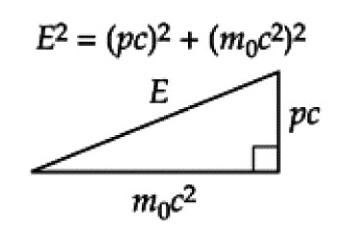
\includegraphics[scale=0.6]{./image/PESTA/general/Einstein.jpg}
		\caption*{\cite{book-2}}
		\label{Einstein}
	\end{figure}
\end{minipage}
\newline
\vspace{.6cm}
\newline
\begin{minipage}[!b]{.5\linewidth}
	\section*{Energia Cinética [Joule]}
	\Large
	$\begin{array}{ l l l }
		E_{c} & = & \frac{1}{2} \; m \; v^{2}
	\end{array}$
\end{minipage}
\begin{minipage}[!b]{.5\linewidth}
	\section*{Energia Potencial [Joule]}
	\Large
	$\begin{array}{ l l l }
		E_{p} & = & \; m \; g \; h
	\end{array}$
\end{minipage}
\newline
\vspace{.6cm}
\newline
\begin{minipage}[l]{\linewidth}
	\section*{Energia Térmica}
	\Large
	$\begin{array}{ l l l l }
		Q - Heat \quad energy & & & \\
		Q_{(t)} - temperature & & & \\
		R - heat \quad resistance & & & \\
		& Q & = & \frac{Q_{1(t)} - Q_{2(t)}}{R}
	\end{array}$
\end{minipage}
%%%%%%%%%%%%%%%%%%%%%%%%%%%%%%%%%%%%%%%%%%%%%%%%%%%%%%%%%%%%%%%%
%%%%%%%%%%%%%%%%%%%%%%%%%%%%%%%%%%%%%%%%%%%%%%%%%%%%%%%%%%%%%%%%
%%%%%%%%%%%%%%%%%%%%%%%%%%%%%%%%%%%%%%%%%%%%%%%%%%%%%%%%%%%%%%%%
%%%%%%%%%%%%%%%%%%%%%%%%%%%%%%%%%%%%%%%%%%%%%%%%%%%%%%%%%%%%%%%%
\begin{comment}
\newline
\vspace{1cm}
\newline
$\frac{A \times B}{C}\times D \approx E$,
\newline
\begin{minipage}{0pt}
	$$\begin{array}{l | l}
		\text{Média aritmetica dados classificados} & \text{Variância de uma amostra dados classificados} \\
		\overline{x} = \frac{1}{n}\sum_{i=1}^cx_in_i = \sum_{i=1}^cx_if_i & s^2 = \frac{1}{n-1}\sum_{i=1}^c (x_i-\bar{x})^2 n_i
	\end{array}$$
\end{minipage}
\newline
\vspace{1cm}
\newline
$IC_{1-\alpha}=\left[ A, B\right]$ ; para $1-\alpha = 0.95$, $\alpha=0.05$, $\frac{\alpha}{2}=0.025$
\newline
\vspace{1cm}
\newline
Zona critica $Z_c=Z_{1-\frac{\alpha}{2}}=\Phi^{-1}(0.975) \cong 1.96$
\newline
\vspace{1cm}
\newline
$P\left( A \leqslant \mu \leqslant B \right) = 1-\alpha$ \\
$\triangle=Z_c\times\frac{\delta}{\sqrt{n}}$ \\
$A = \bar{x}-\triangle \qquad and \qquad B = \bar{x}+\triangle$ \\
$\therefore$\\
$IC_{A_{0.95}}=\left[ \; 18.8877 \: , \: 21.1956 \; \right]$ \hspace{1cm} and \hspace{1cm} $IC_{B_{0.95}}=\left[ \; 20.4519 \: , \: 22.6314 \; \right]$
\newline
\vspace{1cm}
\newline
$\left[ \; \mu \; \right]$
\newline
\vspace{1cm}
\newline
$\bar{y}_{A_0}$ = 6,6111 \qquad $\bar{y}_{B_0}$ = 7,5111 \qquad $n=90$ \\
$\delta_A$ = 2,3112 \qquad $\delta_B$ = 2,5140
\newline
\vspace{1cm}
\newline
$P(Y_A < 6)=P(Y_A \leqslant 5)=F_{i_B}(5) \cong 0,3677 $  \quad e \quad $P(Y_B < 6)=P(Y_B \leqslant 5)=F_{i_B}(5) \cong 0,2444$ \\
\newline
\vspace{1cm}
\newline
$\hat{P_A}-\hat{P_B} \sim N \left( p_A - p_B ; \frac{p_A\:q_A}{n_A} + \frac{p_B\:q_B}{n_B}\right)$ \hspace{1cm}
$\triangle=z_{(1-\frac{\alpha}{2})} \;\sqrt{\frac{\hat{p_A} \: \hat{q_A}}{n_A}+\frac{\hat{p_B} \: \hat{q_B}}{n_B}}$ \hspace{1cm} $q=(1-p)$
\newline
\vspace{1cm}
\newline
$IC_{97\%}(\hat{P_A}-\hat{P_B})=\left[(\hat{p_A}-\hat{p_B})-\triangle \: ; \: (\hat{p_A}-\hat{p_B})+\triangle \right]$
\newline
\vspace{1cm}
\newline
$\hat{P_A}-\hat{P_B} \sim N \left( 0,1233 \; ; \; 0,02788\right)$ \hspace{1cm}
$z_{(1-\frac{\alpha}{2})}=\phi^{-1}(0,985)=2,1701$
\newline
\vspace{1cm}
\newline
Recorrendo a calculadora casio $fx-9860GII$ :
\newline
\vspace{1cm}
\newline
$\triangle= InvNorm(0.985)\sqrt{\frac{0.3677(1-0.3677)}{90}+\frac{0.2444(1-0.2444)}{90}}\: \cong \:0.3677$
\\
$\therefore$
\\
$IC_{97\%}(\hat{P_A}-\hat{P_B})=\left[ \; (\hat{p_A}-\hat{p_B}) \:-\: 0,3624 \: ; \: (\hat{p_A}-\hat{p_B}) \:+\: 0,3624 \; \right]$
\newline
\vspace{1cm}
\newline
\begin{minipage}[l]{0pt}
	$$\left\lbrace\begin{array}{l}
		H_0: \quad \mu_A-\mu_B=0 \\
		\\
		H_1: \quad \mu_A-\mu_B<0
	\end{array}\right.$$
\end{minipage}
\newline
\vspace{1cm}
\newline
\begin{minipage}[l]{0pt}
	$$\left\lbrace\begin{array}{c}
		\mu \;=\; 0 \\
		\delta \;=\; s \\
	\end{array}\right.$$
\end{minipage}
\hspace{3cm} $\Longrightarrow$ \hspace{1cm}
\begin{minipage}[l]{0pt}
	\[\bar{X}=\bar{X}_A-\bar{X}_B \quad \backsim N \left( 0\:,\: \frac{\delta_A^2}{n_A}+\frac{\delta_B^2}{n_B} \right) \quad ; \quad \frac{\delta_A^2}{n_A}+\frac{\delta_B^2}{n_B}\;\cong0.6558 \]
\end{minipage}
\newline
\vspace{1cm}
\newline
$P(\bar{X}_{H_0} \leqslant C)=0.05 \quad \implies \quad RC_X\left] -\infty \:,\: -1.332 \right] \qquad \bar{x}_A-\bar{x}_B=-1.5 \in RC_X $
\newline
\vspace{1cm}
\newline
\begin{minipage}[l]{0pt}
	\[  z_0\:=\: \frac{\bar{x}_A-\bar{x}_B}{\sqrt{\frac{\delta_A^2}{n_A}+\frac{\delta_B^2}{n_B}}}\:\cong\: -1.8523 \qquad
	RC_z \:=\: \left] -\infty \:,\: -1.6448 \right]  \qquad
	pvalue \:=\: P(Z<z_0) \:=\: 0.032 \]
\end{minipage}
\newline
\vspace{1cm}
\newline
\hspace*{5cm} \underline{Condição NEE:}\\
\begin{minipage}[l]{0pt}
	$$\left\lbrace\begin{array}{c}
		\mu \;=\; 0 \\
		\delta \;=\; s \\
	\end{array}\right.$$
\end{minipage}
\hspace{3cm} $\Longrightarrow$ \hspace{1cm}
\begin{minipage}[l]{0pt}
	\[ \bar{Y}=\bar{Y_A}-\bar{Y_B} \quad \backsim N \left( 0\:,\: \frac{\delta_A^2}{n_A}+\frac{\delta_B^2}{n_B} \right) \quad ; \quad \frac{\delta_A^2}{n_A}+\frac{\delta_B^2}{n_B} \; \cong 0.1296 \]
\end{minipage}
\newline
\vspace{1cm}
\newline
$P(\bar{Y}_{H_0} \leqslant C)=0.05 \quad \implies \quad RC_Y\left] -\infty \:,\: -0.5921 \right] \qquad \bar{y}_A-\bar{y}_B=-0.9 \in RC_Y $
\newline
\vspace{1cm}
\newline
\begin{minipage}[l]{0pt}
	\[  z_0\:=\: \frac{\bar{y}_A-\bar{y}_B}{\sqrt{\frac{\delta_A^2}{n_A}+\frac{\delta_B^2}{n_B}}}\:\cong\: -2.5 \qquad
	RC_z \:=\: \left] -\infty \:,\: -1.6448 \right]  \qquad
	pvalue \:=\: P(Z<z_0) \:=\: 0.0062 \]
\end{minipage}
\newline
\vspace{1cm}
\newline
\begin{minipage}[l]{0pt}
	$$\left\lbrace\begin{array}{l}
		H_0: X \backsim N (20.0417\;,\;6.4494^2) \\
		\\
		H_1: X \nsim N (20.0417\;,\;6.4494^2)
	\end{array}\right.$$
\end{minipage}
\newline
\vspace{1cm}
\newline
\hspace*{5cm} \underline{NEE Região B:} \\
\begin{minipage}[l]{0pt}
	$$\left\lbrace\begin{array}{l}
		H_0: X \backsim N (7.5111\;,\;2.5140^2) \\
		\\
		H_1: X \nsim N (7.5111\;,\;2.5140^2)
	\end{array}\right.$$
\end{minipage}
\newline
\vspace{1cm}
\newline
$q_0=\sum_{i=1}^n \frac{(n_i-e_i)^2}{e_i} \;\backsim\; \chi_{(k-m-1)}^2$
\newline
\vspace{1cm}
\newline
$RC_{\chi^2}=\left[ \: InvChiCD(0.05,5) \:,\: +\infty \; \right] \quad \rightarrow \quad RC_{\chi_2}=\left[ \: 11.0705 \:,\: +\infty \; \right]$
\newline
\vspace{1cm}
\newline
$q_0=8.5532$ < 11.0705
\newline
\vspace{1cm}
\newline
$\left[ \; \mu \; \right]$
\newline
\vspace{1cm}
\newline
$\bar{y}_{A_0}$ = 6,6111 \qquad $\bar{y}_{B_0}$ = 7,5111 \qquad $n=90$ \\
$\delta_A$ = 2,3112 \qquad $\delta_B$ = 2,5140
\newline
\vspace{1cm}
\newline
$P(Y_A < 6)=P(Y_A \leqslant 5)=F_{i_B}(5) \cong 0,3677 $  \quad e \quad $P(Y_B < 6)=P(Y_B \leqslant 5)=F_{i_B}(5) \cong 0,2444$
\newline
\vspace{1cm}
\newline
$\hat{P_A}-\hat{P_B} \sim N \left( p_A - p_B ; \frac{p_A\:q_A}{n_A} + \frac{p_B\:q_B}{n_B}\right)$ \hspace{1cm}
$\triangle=z_{(1-\frac{\alpha}{2})} \;\sqrt{\frac{\hat{p_A} \: \hat{q_A}}{n_A}+\frac{\hat{p_B} \: \hat{q_B}}{n_B}}$ \hspace{1cm} $q=(1-p)$
\newline
\vspace{1cm}
\newline
$IC_{97\%}(\hat{P_A}-\hat{P_B})=\left[(\hat{p_A}-\hat{p_B})-\triangle \: ; \: (\hat{p_A}-\hat{p_B})+\triangle \right]$
\newline
\vspace{1cm}
\newline
$\hat{P_A}-\hat{P_B} \sim N \left( 0,1233 \; ; \; 0,02788\right)$ \hspace{1cm}
$z_{(1-\frac{\alpha}{2})}=\phi^{-1}(0,985)=2,1701$
\newline
\vspace{1cm}
\newline
Recorrendo a calculadaora casio $fx-9860GII$ :
\newline
\vspace{1cm}
\newline
$\triangle= InvNorm(0.985)\sqrt{\frac{0.3677(1-0.3677)}{90}+\frac{0.2444(1-0.2444)}{90}}\: \cong \:0.3677$
\\
$\therefore$
\\
$IC_{97\%}(\hat{P_A}-\hat{P_B})=\left[ \; (\hat{p_A}-\hat{p_B}) \:-\: 0,3624 \: ; \: (\hat{p_A}-\hat{p_B}) \:+\: 0,3624 \; \right]$
\newline
\vspace{1cm}
\newline
\begin{minipage}[l]{0pt}
	$$\left\lbrace\begin{array}{l}
		H_0: \quad \mu_A-\mu_B=0 \\
		\\
		H_1: \quad \mu_A-\mu_B<0
	\end{array}\right.$$
\end{minipage}
\newline
\vspace{1cm}
\newline
\begin{minipage}[l]{0pt}
	$$\left\lbrace\begin{array}{c}
		\mu \;=\; 0 \\
		\delta \;=\; s \\
	\end{array}\right.$$
\end{minipage}
\hspace{3cm} $\Longrightarrow$ \hspace{1cm}
\begin{minipage}[l]{0pt}
	\[\bar{X}=\bar{X}_A-\bar{X}_B \quad \backsim N \left( 0\:,\: \frac{\delta_A^2}{n_A}+\frac{\delta_B^2}{n_B} \right) \quad ; \quad \frac{\delta_A^2}{n_A}+\frac{\delta_B^2}{n_B}\;\cong0.6558 \]
\end{minipage}
\newline
\vspace{1cm}
\newline
$P(\bar{X}_{H_0} \leqslant C)=0.05 \quad \implies \quad RC_X\left] -\infty \:,\: -1.332 \right] \qquad \bar{x}_A-\bar{x}_B=-1.5 \in RC_X $
\newline
\vspace{1cm}
\newline
\begin{minipage}[l]{0pt}
	\[  z_0\:=\: \frac{\bar{x}_A-\bar{x}_B}{\sqrt{\frac{\delta_A^2}{n_A}+\frac{\delta_B^2}{n_B}}}\:\cong\: -1.8523 \qquad
	RC_z \:=\: \left] -\infty \:,\: -1.6448 \right]  \qquad
	pvalue \:=\: P(Z<z_0) \:=\: 0.032 \]
\end{minipage}
\newline
\vspace{1cm}
\newline
\hspace*{5cm} \underline{Condição NEE:}\\
\begin{minipage}[l]{0pt}
	$$\left\lbrace\begin{array}{c}
		\mu \;=\; 0 \\
		\delta \;=\; s \\
	\end{array}\right.$$
\end{minipage}
\hspace{3cm} $\Longrightarrow$ \hspace{1cm}
\begin{minipage}[l]{0pt}
	\[ \bar{Y}=\bar{Y_A}-\bar{Y_B} \quad \backsim N \left( 0\:,\: \frac{\delta_A^2}{n_A}+\frac{\delta_B^2}{n_B} \right) \quad ; \quad \frac{\delta_A^2}{n_A}+\frac{\delta_B^2}{n_B} \; \cong 0.1296 \]
\end{minipage}
\newline
\vspace{1cm}
\newline
$P(\bar{Y}_{H_0} \leqslant C)=0.05 \quad \implies \quad RC_Y\left] -\infty \:,\: -0.5921 \right] \qquad \bar{y}_A-\bar{y}_B=-0.9 \in RC_Y $
\newline
\vspace{1cm}
\newline
\begin{minipage}[l]{0pt}
	\[  z_0\:=\: \frac{\bar{y}_A-\bar{y}_B}{\sqrt{\frac{\delta_A^2}{n_A}+\frac{\delta_B^2}{n_B}}}\:\cong\: -2.5 \qquad
	RC_z \:=\: \left] -\infty \:,\: -1.6448 \right]  \qquad
	pvalue \:=\: P(Z<z_0) \:=\: 0.0062 \]
\end{minipage}
\newline
\vspace{1cm}
\newline
\begin{minipage}[l]{0pt}
	$$\left\lbrace\begin{array}{l}
		H_0: X \backsim N (20.0417\;,\;6.4494^2) \\
		\\
		H_1: X \nsim N (20.0417\;,\;6.4494^2)
	\end{array}\right.$$
\end{minipage}
\newline
\vspace{1cm}
\newline
\hspace*{5cm} \underline{NEE Região B:} \\
\begin{minipage}[l]{0pt}
	$$\left\lbrace\begin{array}{l}
		H_0: X \backsim N (7.5111\;,\;2.5140^2) \\
		\\
		H_1: X \nsim N (7.5111\;,\;2.5140^2)
	\end{array}\right.$$
\end{minipage}
\newline
\vspace{1cm}
\newline
$q_0=\sum_{i=1}^n \frac{(n_i-e_i)^2}{e_i} \;\backsim\; \chi_{(k-m-1)}^2$
\newline
\vspace{1cm}
\newline
$RC_{\chi^2}=\left[ \: InvChiCD(0.05,5) \:,\: +\infty \; \right] \quad \rightarrow \quad RC_{\chi_2}=\left[ \: 11.0705 \:,\: +\infty \; \right]$
\newline
\vspace{1cm}
\newline
$q_0=8.5532$ < 11.0705
\newline
\vspace{1cm}
\newline
\begin{minipage}[l]{0pt}
	$$\left\lbrace\begin{array}{l}
		H_0: \bar{X}_{H_0} \backsim N (0 \;,\; 0.6558) \\
		\\
		H_1: \bar{X}_{H_1} \backsim N (-1.5 \;,\; 0.6558)
	\end{array}\right.$$
\end{minipage}
\newline
\vspace{1cm}
\newline
$\beta=P(Aceitar H_0 | H_0 é Falsa)$ \\
$\beta=(\bar{X}_{H_1} \:>\: -1.332)$	\\
$\beta=NormCD(-1.332,99999999,\sqrt{0.6558},-1.5)=0.4178$ \\
Potência do teste \\
$1-\beta=P(Rejeitar H_0 | H_0 é Falsa)=0.5822$
\newline
\vspace{1cm}
\newline
NEE Região B:\\
\begin{minipage}[l]{0pt}
	$$\left\lbrace\begin{array}{l}
		H_0: \bar{Y}_{H_0} \backsim N (0 \;,\; 0.1296) \\
		\\
		H_1: \bar{Y}_{H_1} \backsim N (-0.9 \;,\; 0.1296)
	\end{array}\right.$$
\end{minipage}
\newline
\vspace{1cm}
\newline
$\beta=P(Aceitar H_0 | H_0 é Falsa)$ \\
$\beta=(\bar{Y}_{H_1} \:>\: -0.5921)$	\\
$\beta=NormCD(-0.5921,99999999,\sqrt{0.1296},-0.9)=0.1962$ \\
Potência do teste \\
$1-\beta=P(Rejeitar H_0 | H_0 é Falsa)=0.8038$
\newline
\vspace{1cm}
\newline
$\chi^2$
\end{comment}
%%%%%%%%%%%%%%%%%%%%%%%%%%%%%%%%%%%%%%%%%%%%%%%%%%%%%%%%%%%%%%%%

%%%%%%%%%%%%%%%%%%%%%%%%%%%%%%%%%%%%%%%%%%%%%%%%%%%%%%%%%%%%%%%%%
\newgeometry{top=1cm,left=1cm,right=.3cm,bottom=.3cm}
\chapter{Código}
{
	\fontfamily{pcr}
	\small
	\section*{main}
	\label{anexo-main}
	%\begin{verbatimtab}
\begin{lstlisting}[language=C, caption={main.c}, label=main-c, captionpos=b]
/************************************************************************
Title: BALANCA COMERCIAL
Author: Sergio Manuel Santos
<sergio.salazar.santos@gmail.com>
File: $Id: MAIN,v 1.8.2.1 21/02/2021 Exp $
License: GNU General Public License
Software: Atmel Studio 7 (ver 7.0.129)
Hardware: Atmega128 by ETT ET-BASE
-PORTA LCD
-PORTF pin 6,7 HX711, pin 0 to 5 Buttons, 
PIN 0 -> OFFSET, 
PIN 3 -> DEFAULT 5sec press, and up count for div factor, 
PIN 4 -> ENTER GAIN FACTOR MENU 5 sec press, and down count for div factor, 
PIN 5 -> ENTER KEY to validate entered value and put in effect.
PIN 6 and 7 -> dedicated to comunicate with Signal Amplifier
-PORTC status indicator leds
PIN 5 -> Indicate using stored values
PIN 6 -> Reset to default indicator (blinks four times)
PIN 7 -> In Calibration Menu (on)
Comment:
nice
************************************************************************/
#define F_CPU 16000000UL
/*
** library
*/
#include <avr/io.h>
#include <avr/pgmspace.h>
#include <avr/interrupt.h>
#include <util/delay.h>
#include <math.h>
#include <inttypes.h>
#include <stdlib.h>
#include <string.h>
#include "explode.h"
//#include "atmega128interrupt.h"
#include "atmega128timer.h"
#include "function.h"
#include "lcd.h"
#include "hx711.h"
#include "eeprom.h"
/*
** Constant and Macro
*/
#ifndef STATUS_REGISTER
#define STATUS_REGISTER SREG
#define GLOBAL_INTERRUPT_ENABLE 7
#endif
#define ZERO 0
#define ONE 1
#define TRUE 1
#define average_n 24 //64 -> 24
#define blink 8
#define IMASK 0x3F
#define _5sec 5
#define _10sec 10
#define minDIV 1
#define maxDIV 255
/*
** Global File variable
*/
EXPLODE F;
LCD0 lcd0;
TIMER_COUNTER0 timer0;
//INTERRUPT intx;
HX711_calibration HX711_data;
HX711_calibration* HX711_ptr;
const uint8_t sizeblock = sizeof(HX711_calibration);
HX711 hx;
float tmp;
EEPROM eprom;
char result[32];
char Menu = '1'; // Main menu selector
uint8_t counter_1 = ZERO;
uint8_t counter_2 = ZERO;
uint8_t signal = ZERO;
uint8_t count=blink;
uint16_t divfactor;
/*
** Header
*/
void PORTINIT();
/****MAIN****/
int main(void)
{
	PORTINIT();
	HX711_ptr = &HX711_data; // CALIBRATION DATA BUS
	/***INICIALIZE OBJECTS***/
	F = EXPLODEenable();
	FUNC function = FUNCenable();
	lcd0 = LCD0enable(&DDRA,&PINA,&PORTA);
	timer0 = TIMER_COUNTER0enable(2,2); //2,2
	TIMER_COUNTER1 timer1 = TIMER_COUNTER1enable(4,2); //4,2
	hx = HX711enable(&DDRF, &PINF, &PORTF, 6, 7); //6,7
	eprom = EEPROMenable();
	//intx = INTERRUPTenable();
	/******/
	float value = 0;
	float publish = 0;
	uint8_t choice;
	// Get default values to buss memory
	HX711_data.offset_32 = hx.get_cal(&hx)->offset_32;
	HX711_data.offset_64 = hx.get_cal(&hx)->offset_64;
	HX711_data.offset_128 = hx.get_cal(&hx)->offset_128;
	HX711_data.divfactor_32 = hx.get_cal(&hx)->divfactor_32;
	HX711_data.divfactor_64 = hx.get_cal(&hx)->divfactor_64;
	HX711_data.divfactor_128 = hx.get_cal(&hx)->divfactor_128;
	HX711_data.status = hx.get_cal(&hx)->status;
	/***Parameters timers***/
	timer0.compoutmode(1); // troubleshooting blinking PORTB 5
	/***79 and 8  -> 80 us***/
	timer0.compare(60); // 8 -> 79 -> 80 us, fine tunned = 8 -> 60 -> 30.4us
	timer0.start(8); // 1 -> 32 us , 8 -> 256 us , 32 64 128 256 1024
	// to be used to jump menu for calibration in progress
	timer1.compoutmodeA(1); // troubleshooting blinking PORTB 6
	timer1.compareA(62800); // Freq = 256 -> 62800 -> 2 s
	timer1.start(256);
	//intx.set(1,0); // Not necessary, if used move IDC from PORTF to PORTD with new config pinage.
	// HX711 Gain
	hx.set_amplify(&hx, 64); // 32 64 128
	choice = hx.get_amplify(&hx);
	if(choice == 1)
	divfactor = (uint16_t) HX711_data.divfactor_128;
	if(choice == 2)
	divfactor = (uint16_t) HX711_data.divfactor_32;
	if(choice == 3)
	divfactor = (uint16_t) HX711_data.divfactor_64;
	//Get stored calibration values and put them to effect
	eprom.read_block(HX711_ptr, (const void*) ZERO, sizeblock);
	if(HX711_ptr->status == 1){
		//Load stored value 
		hx.get_cal(&hx)->offset_32 = HX711_ptr->offset_32;
		hx.get_cal(&hx)->offset_64 = HX711_ptr->offset_64;
		hx.get_cal(&hx)->offset_128 = HX711_ptr->offset_128;
		hx.get_cal(&hx)->divfactor_32 = HX711_ptr->divfactor_32;
		hx.get_cal(&hx)->divfactor_64 = HX711_ptr->divfactor_64;
		hx.get_cal(&hx)->divfactor_128 = HX711_ptr->divfactor_128;
		hx.get_cal(&hx)->status=ZERO;
		PORTC &= ~(ONE << 5); // troubleshooting
	}
	/*********************************************************/
	//lcd0.gotoxy(1,0); // for troubleshooting
	//lcd0.string_size(function.ftoa(HX711_data.status, result, ZERO), 13);
	//lcd0.string_size(function.ftoa(hx.get_cal(&hx)->offset_64, result, ZERO), 13);
	/*********************************************************/
	while(TRUE){
		/******PREAMBLE******/
		lcd0.reboot(); //Reboot LCD
		F.boot(&F,PINF); //PORTF INPUT READING
		/************INPUT***********/
		if(hx.query(&hx)) //Catches falling Edge instance, begins bit shifting.
		continue;
		/***geting data interval***/
		// Jump Menu signal
		if(signal == ONE){ //INPUT FROM INTERRUPT SINALS
			Menu = '2';
			signal = ZERO; // ONE SHOT
			lcd0.clear();
		}
		tmp = hx.raw_average(&hx, average_n); // average_n  25 or 50, smaller means faster or more readings
		/****************************/
		switch(Menu){
			/***MENU 1***/
			case '1': // Main Program Menu
			lcd0.gotoxy(0,4); //TITLE
			lcd0.string_size("Weight Scale", 12); //TITLE
			/*********************************************/
			//lcd0.gotoxy(1,0); // for troubleshooting
			//lcd0.string_size(function.ftoa(hx.read_raw(&hx), result, ZERO), 13);
			/*********************************************/
			if((F.hl(&F) & IMASK) & ONE){ // calibrate offset by pressing button 1
				HX711_data.offset_32 = tmp;
				HX711_data.offset_64 = tmp;
				HX711_data.offset_128 = tmp;
				HX711_data.status = ONE;
				eprom.update_block(HX711_ptr, (void*) ZERO, sizeblock);
				hx.get_cal(&hx)->offset_32 = HX711_ptr->offset_32;
				hx.get_cal(&hx)->offset_64 = HX711_ptr->offset_64;
				hx.get_cal(&hx)->offset_128 = HX711_ptr->offset_128;
				hx.get_cal(&hx)->status=ZERO;
				PORTC &= ~(ONE << 5);
			}
			if(choice == 1 || choice == 11)
			value = (tmp - hx.get_cal(&hx)->offset_128) / hx.get_cal(&hx)->divfactor_128; //value to be published to LCD
			if(choice == 2 || choice == 21)
			value = (tmp - hx.get_cal(&hx)->offset_32) / hx.get_cal(&hx)->divfactor_32; //value to be published to LCD
			if(choice == 3 || choice == 31)
			value = (tmp - hx.get_cal(&hx)->offset_64) / hx.get_cal(&hx)->divfactor_64; //value to be published to LCD
			/*********************************************/
			//lcd0.gotoxy(3,0); // for troubleshooting
			//lcd0.string_size(function.ftoa(tmp, result, ZERO), 13);
			//lcd0.string_size(function.ftoa(hx.get_cal(&hx)->divfactor_128, result, ZERO), 13);
			//lcd0.string_size(function.ftoa(hx.get_cal(&hx)->offset_128, result, ZERO), 13);
			/*********************************************/
			if (value > 1000 || value < -1000){
				publish = value / 1000;
				lcd0.gotoxy(2,1);
				lcd0.string_size(function.ftoa(publish, result, 3), 13); lcd0.string_size("Kg", 4);
			}else{
				publish = value;
				lcd0.gotoxy(2,1);
				lcd0.string_size(function.ftoa(publish, result, ZERO), 13); lcd0.string_size("gram", 4);
			}
			break;
			/***MENU 2***/
			case '2': // MANUAL CALIBRATE DIVFACTOR MENU
			/**/
			lcd0.gotoxy(0,1);
			lcd0.string_size("SETUP GAIN FACTOR",17);
			switch(choice){
				case 1: // case 128
				divfactor=hx.get_cal(&hx)->divfactor_128;
				choice=11;
				break;
				case 11: // case 128
				lcd0.gotoxy(2,9);
				if(F.hl(&F) == (ONE << 3)){
					divfactor++;
					if(divfactor > maxDIV)
					divfactor = maxDIV;
				}
				if(F.hl(&F) == (ONE << 4)){
					divfactor--;
					if(divfactor < minDIV)
					divfactor = minDIV;
				}
				HX711_data.divfactor_128 = divfactor;
				lcd0.string_size(function.ui16toa(divfactor),6);
				break;
				case 2: // case 32
				divfactor=hx.get_cal(&hx)->divfactor_32;
				choice=21;
				break;
				case 21: // case 32
				lcd0.gotoxy(2,9);
				if(F.hl(&F) == (ONE << 3)){
					divfactor++;
					if(divfactor > maxDIV)
					divfactor = maxDIV;
				}
				if(F.hl(&F) == (ONE << 4)){
					divfactor--;
					if(divfactor < minDIV)
					divfactor=minDIV;
				}
				HX711_data.divfactor_32 = divfactor;
				lcd0.string_size(function.ui16toa(divfactor),6);
				break;
				case 3: // case 64
				divfactor=hx.get_cal(&hx)->divfactor_64;
				choice=31;
				break;
				case 31: // case 64
				lcd0.gotoxy(2,9);
				if(F.hl(&F) == (ONE << 3)){
					divfactor++;
					if(divfactor > maxDIV)
					divfactor = maxDIV;
				}
				if(F.hl(&F) == (ONE << 4)){
					divfactor--;
					if(divfactor < minDIV)
					divfactor = minDIV;
				}
				HX711_data.divfactor_64 = divfactor;
				lcd0.string_size(function.ui16toa(divfactor),6);
				break;
				default:
				choice = 3;
				break;
			};
			// Exit and store value
			if((F.ll(&F) & IMASK) == (ONE << 5)){ // Button 6
				HX711_data.status = ONE;
				eprom.update_block(HX711_ptr, (void*) ZERO, sizeblock);
				hx.get_cal(&hx)->divfactor_32=divfactor;
				hx.get_cal(&hx)->divfactor_64=divfactor;
				hx.get_cal(&hx)->divfactor_128=divfactor;
				hx.get_cal(&hx)->status=ZERO;
				PORTC &= ~(ONE << 5); // troubleshooting
				PORTC |= (ONE << 7); // troubleshooting
				counter_2 = ZERO;
				Menu = '1';
				lcd0.clear();
			}
			/**/
			break;
			/********************************************************************/
			default:
			Menu = '1';
			break;
		};
	}
}
/*
** procedure and function
*/
void PORTINIT(void)
{
	//Control buttons
	PORTF |= IMASK;
	//troubleshooting output
	DDRC = 0xFF;
	PORTC = 0xFF;
}
/*
** interrupt
*/
ISR(TIMER0_COMP_vect) // 15.4 us intervals
{
	/***Block other interrupts during this procedure***/
	uint8_t Sreg;
	Sreg = STATUS_REGISTER;
	STATUS_REGISTER &= ~(ONE << GLOBAL_INTERRUPT_ENABLE);
	hx.read_raw(&hx);
	/***enable interrupts again***/
	STATUS_REGISTER = Sreg;
}
ISR(TIMER1_COMPA_vect) // 1 second intervals
{
	/***CLEAR EEPROM OFFSET SEQUENCE START***/
	if((F.ll(&F) & IMASK) == (ONE << 3)) //button 4
	counter_1++;
	else if(counter_1 < _5sec+ONE)
	counter_1=ZERO;
	if(counter_1 > _5sec){
		counter_1 = _5sec+ONE; //lock in place
		PORTC ^= (ONE << 6); // troubleshooting
		count--;
		if(!count){ //led blinks x times
			// Delete eeprom memory ZERO
			eprom.update_block(HX711_Default, (void*) ZERO, sizeblock);
			hx.get_cal(&hx)->offset_32 = HX711_Default->offset_32;
			hx.get_cal(&hx)->offset_64 = HX711_Default->offset_64;
			hx.get_cal(&hx)->offset_128 = HX711_Default->offset_128;
			hx.get_cal(&hx)->divfactor_32 = divfactor = HX711_Default->divfactor_32;
			hx.get_cal(&hx)->divfactor_64 = divfactor = HX711_Default->divfactor_64;
			hx.get_cal(&hx)->divfactor_128 = HX711_Default->divfactor_128;
			hx.get_cal(&hx)->status = HX711_Default->status;
			PORTC |= (ONE << 5); // troubleshooting
			PORTC |= (ONE << 6); // troubleshooting
			counter_1 = ZERO;
			count=blink;
		}
	}
	/***CLEAR EEPROM OFFSET SEQUENCE END***/
	/***CAL DIVFACTOR DEFINE START***/
	if((F.ll(&F) & IMASK) == (ONE << 4)) //button 5
	counter_2++;
	else if(counter_2 < _5sec+ONE)
	counter_2=ZERO; //RESET TIMER
	if(counter_2 > _5sec){
		counter_2 = ZERO; //RESET TIMER
		signal = ONE;
		PORTC &= ~(ONE << 7); // troubleshooting
	}
	/***CAL DIVFACTOR DEFINE END***/
}
/***EOF***/
/**** Comment:
because 24 bit will have to create a vector pointer of the size of 32 bit, then at the end do a cast to *((int32_t*)ptr).

Endurance test over 2 months, noticed drift during days, but never getting over 20 grams. For a scale using a 50Kg cell is Excellent.
Using offset corrects the drift and precision is concise to the gram.
****/
\end{lstlisting}
%\end{verbatimtab}
%%%%%%%%%%%%%%%%%%%%%%%%%%%%%%%%%%%%%%%%%%%%%%%%%%%%%%%%%%%%%%%%


	\newpage
	\section*{explode.h}
	\label{anexo-explode-h}
	\begin{verbatimtab}
/************************************************************************
EXPLODE
Author: Sergio Santos
<sergio.salazar.santos@gmail.com>
License: GNU General Public License
Hardware: all
Date: 16032021
Comment:

************************************************************************/
#ifndef _EXPLODE_H_
	#define _EXPLODE_H_
	/***Library***/
	#include <inttypes.h>
	/***Constant & Macro***/
	/***Global Variable***/
	struct expld{
		/***Variable***/
		unsigned int XI;
		unsigned int XF;
		/***PROTOTYPES VTABLE***/
		void (*boot)(struct expld* self, uint8_t x);
		uint8_t (*mayia)(struct expld* self, uint8_t nbits);
		uint8_t (*hh)(struct expld* self);
		uint8_t (*ll)(struct expld* self);
		uint8_t (*lh)(struct expld* self);
		uint8_t (*hl)(struct expld* self);
		uint8_t (*diff)(struct expld* self);
		uint8_t (*data)(struct expld* self);
	};
	typedef struct expld EXPLODE;
	/***Header***/
	EXPLODE EXPLODEenable(void);
#endif
/***Comment***
*************/
/***EOF***/
\end{verbatimtab}
	\newpage
	\section*{explode.c}
	\label{anexo-explode-c}
	\begin{verbatimtab}
/********************************************************************
EXPLODE
Author: Sergio Santos
<sergio.salazar.santos@gmail.com> 
License: GNU General Public License
Hardware: all
Date: 16032021
Comment:
Pin Analysis
********************************************************************/
/***Library***/
#include <avr/io.h>
#include <inttypes.h>
#include"explode.h"
/***Constant & Macro***/
#ifndef GLOBAL_INTERRUPT_ENABLE
	#define STATUS_REGISTER SREG
	#define GLOBAL_INTERRUPT_ENABLE 7
#endif
#define ZERO 0
#define ONE 1
/***Global File Variable***/
/***Header***/
uint8_t EXPLODEPwr(uint8_t bs, uint8_t n);
/************/
void EXPLODEboot(EXPLODE* self, uint8_t x);
uint8_t EXPLODEmayia(EXPLODE* self, uint8_t nbits);
uint8_t EXPLODEhh(EXPLODE* self);
uint8_t EXPLODEll(EXPLODE* self);
uint8_t EXPLODElh(EXPLODE* self);
uint8_t EXPLODEhl(EXPLODE* self);
uint8_t EXPLODEdiff(EXPLODE* self);
uint8_t EXPLODEdata(EXPLODE* self);
/***Procedure & Function***/
EXPLODE EXPLODEenable( void )
{
	uint8_t tSREG;
	tSREG = STATUS_REGISTER;
	STATUS_REGISTER &= ~(ONE<<GLOBAL_INTERRUPT_ENABLE);
	// struct object
	struct expld explode;
	// inic VAR
	explode.XI = ZERO;
	explode.XF = ZERO;
	// function pointers
	explode.boot = EXPLODEboot;
	explode.mayia = EXPLODEmayia;
	explode.hh = EXPLODEhh;
	explode.ll = EXPLODEll;
	explode.lh = EXPLODElh;
	explode.hl = EXPLODEhl;
	explode.diff = EXPLODEdiff;
	explode.data = EXPLODEdata;
	STATUS_REGISTER = tSREG;
	/******/
	return explode;
}
// boot
void EXPLODEboot(EXPLODE* self, uint8_t x)
{
	self->XI = self->XF;
	self->XF = x;
}
// mayia
uint8_t EXPLODEmayia(EXPLODE* self, uint8_t nbits)
{//magic formula
	unsigned int mask;
	unsigned int diff;
	unsigned int trans;
	mask = EXPLODEPwr(2,nbits)-ONE;
	self->XI &= mask;
	self->XF &= mask;
	diff = self->XF ^ self->XI;
	trans = diff & self->XF;
	return (trans << nbits) | diff;
}
// hh
uint8_t EXPLODEhh(EXPLODE* self)
{
	uint8_t i;
	i = self->XI & self->XF;
	return i;
}
// ll
uint8_t EXPLODEll(EXPLODE* self)
{
	uint8_t i;
	i = self->XI | self->XF;
	return ~i;
}
// lh
uint8_t EXPLODElh(EXPLODE* self)
{
	uint8_t i;
	i = self->XI ^ self->XF;
	i &= self->XF;
	return i;
}
// hl
uint8_t EXPLODEhl(EXPLODE* self)
{
	uint8_t i;
	i = self->XF ^ self->XI;
	i &= self->XI;
	return i;
}
// diff
uint8_t EXPLODEdiff(EXPLODE* self)
{
	return self->XF ^ self->XI;
}
uint8_t EXPLODEdata(EXPLODE* self)
{
	return self->XF;	
}
/*******************************************************************/
// power: raise base to n-th power; n >= 0
uint8_t EXPLODEPwr(uint8_t bs, uint8_t n)
{
	uint8_t i, p;
	p = ONE;
	for (i = ONE; i <= n; ++i)
		p = p * bs;
	return p;
}
/***Interrupt***/
/***Comment***
*************/
/***EOF***/
\end{verbatimtab}
	\newpage
	\section*{atmega128interrupt.h}
	\label{anexo-atmega128interrupt-h}
	\begin{verbatimtab}
/************************************************************************
ATMEGA128INTERRUPT
Author: Sergio Santos 
<sergio.salazar.santos@gmail.com>
Hardware: ATmega128
Date: 25102020
Comment:
Stable
************************************************************************/
/***Preamble Inic***/
#ifndef _ATMEGA128INTERRUPT_H_
#define _ATMEGA128INTERRUPT_H_
/**@{*/
#if (__GNUC__ * 100 + __GNUC_MINOR__) < 304
	#error "This library requires AVR-GCC 3.4 or later, update to newer AVR-GCC compiler !"
#endif
/***Library***/
#include <inttypes.h>
/***Constant & Macro***/
/***Global Variable***/
struct ntrrpt{
	void (*set)(uint8_t channel, uint8_t sense);
	void (*off)(uint8_t channel);
	void (*on)(uint8_t channel);
	uint8_t (*reset_status)(void);
};
typedef struct ntrrpt INTERRUPT;
/***Header***/
INTERRUPT INTERRUPTenable(void);
#endif
/***EOF***/
\end{verbatimtab}
	\newpage
	\section*{atmega128interrupt.c}
	\label{anexo-atmega128interrupt-c}
	%\begin{verbatimtab}
\begin{lstlisting}[language=C, caption={atmega128interrupt.c}, label=atmega128interrupt-c, captionpos=b]
/*************************************************************************
ATMEGA128INTERRUPT
Author: Sergio Santos 
<sergio.salazar.santos@gmail.com>
Hardware: ATmega128
Date: 25102020
Comment:
Stable
*************************************************************************/
/***Preamble Inic***/
#ifndef F_CPU
	#define F_CPU 16000000UL
#endif
/***Library***/
#include <avr/io.h>
#include <avr/interrupt.h>
#include <avr/pgmspace.h>
#include <stdarg.h>
#include "atmega128interrupt.h"
/***Constant & Macro***/
#ifndef GLOBAL_INTERRUPT_ENABLE
	#define GLOBAL_INTERRUPT_ENABLE 7
#endif
#if defined(__AVR_ATmega64__) || defined(__AVR_ATmega128__)	
	/***/
	#define ATMEGA_INTERRUPT
	#define External_Interrupt_Control_Register_A EICRA
	#define External_Interrupt_Control_Register_B EICRB
	#define External_Interrupt_Mask_Register EIMSK
	#define External_Interrupt_Flag_Register EIFR
	#define MCU_Control_Status_Register MCUCSR
	#define MCU_Control_Status_Register_Mask 0X1F
#else
	#error "Not Atmega 128"
#endif
/***Gloabal File Variables***/
/***Header***/
void INTERRUPT_set(uint8_t channel, uint8_t sense);
void INTERRUPT_off(uint8_t channel);
void INTERRUPT_on(uint8_t channel);
uint8_t INTERRUPT_reset_status(void);
/***Procedure & Function***/
INTERRUPT INTERRUPTenable(void)
/***
Setup blank
***/
{
INTERRUPT interrupt;
External_Interrupt_Mask_Register = 0X00;
/******/
interrupt.set=INTERRUPT_set;
interrupt.off=INTERRUPT_off;
interrupt.on=INTERRUPT_on;
interrupt.reset_status=INTERRUPT_reset_status;
return interrupt;
}
uint8_t INTERRUPT_reset_status(void)
{
uint8_t reset, ret=0;
reset=(MCU_Control_Status_Register & MCU_Control_Status_Register_Mask);
switch(reset){
	case 1: // Power-On Reset Flag
		ret=0;
		MCU_Control_Status_Register &= ~(1<<PORF);
		break;
	case 2: // External Reset Flag
		MCU_Control_Status_Register &= ~(1<<EXTRF);
		ret=1;
		break;
	case 4: // Brown-out Reset Flag
		MCU_Control_Status_Register &= ~(1<<BORF);
		ret=2;
		break;
	case 8: // Watchdog Reset Flag
		MCU_Control_Status_Register &= ~(1<<WDRF);
		ret=3;
		break;
	case 16: // JTAG Reset Flag
		MCU_Control_Status_Register &= ~(1<<JTRF);
		ret=4;
		break;
	default: // clear all status
		MCU_Control_Status_Register &= ~(MCU_Control_Status_Register_Mask);
		break;
}
return ret;
}
void INTERRUPT_set(uint8_t channel, uint8_t sense)
{
switch( channel ){
	case 0: 
		External_Interrupt_Mask_Register &= ~(1<<INT0);
		External_Interrupt_Control_Register_A &= ~((1<<ISC01) |
		(1<<ISC00));
		switch(sense){
			case 0: // The low level of INTn generates an interrupt request.
			case 1: // The low level of INTn generates an interrupt request.
				break;
			case 2: 
			// The falling edge of INTn generates asynchronously an interrupt request.
				External_Interrupt_Control_Register_A |= (1<<ISC01);
				break;
			case 3: 
			// The rising edge of INTn generates asynchronously an interrupt request.
				External_Interrupt_Control_Register_A |= ((1<<ISC01) | (1<<ISC00));
				break;
			default: // The low level of INTn generates an interrupt request.
				break;
		}
	External_Interrupt_Mask_Register |= (1<<INT0);
	break;
	case 1:
		External_Interrupt_Mask_Register &= ~(1<<INT1);
		External_Interrupt_Control_Register_A &= ~((1<<ISC11) | (1<<ISC10));
		switch(sense){
			case 0: // The low level of INTn generates an interrupt request.
			case 1: // The low level of INTn generates an interrupt request.
				break;
			case 2: 
			// The falling edge of INTn generates asynchronously an interrupt request.
				External_Interrupt_Control_Register_A |= (1<<ISC11);
				break;
			case 3: 
			// The rising edge of INTn generates asynchronously an interrupt request.
				External_Interrupt_Control_Register_A |= ((1<<ISC11) | (1<<ISC10));
				break;
			default: // The low level of INTn generates an interrupt request.
				break;
		}
		External_Interrupt_Mask_Register |= (1<<INT1);
		break;
	case 2:
		External_Interrupt_Mask_Register &= ~(1<<INT2);
		External_Interrupt_Control_Register_A &= ~((1<<ISC21) | (1<<ISC20));
		switch(sense){
			case 0: // The low level of INTn generates an interrupt request.
			case 1: // The low level of INTn generates an interrupt request.
				break;
			case 2: 
			// The falling edge of INTn generates asynchronously an interrupt request.
				External_Interrupt_Control_Register_A |= (1<<ISC21);
				break;
			case 3: 
			// The rising edge of INTn generates asynchronously an interrupt request.
				External_Interrupt_Control_Register_A |= ((1<<ISC21) | (1<<ISC20));
				break;
			default: // The low level of INTn generates an interrupt request.
				break;
		}
		External_Interrupt_Mask_Register |= (1<<INT2);
		break;
	case 3:
		External_Interrupt_Mask_Register &= ~(1<<INT3);
		External_Interrupt_Control_Register_A &= ~((1<<ISC31) | (1<<ISC30));
		switch(sense){
			case 0: // The low level of INTn generates an interrupt request.
			case 1: // The low level of INTn generates an interrupt request.
				break;
			case 2: 
			// The falling edge of INTn generates asynchronously an interrupt request.
				External_Interrupt_Control_Register_A |= (1<<ISC31);
				break;
			case 3: 
			// The rising edge of INTn generates asynchronously an interrupt request.
				External_Interrupt_Control_Register_A |= ((1<<ISC31) | (1<<ISC30));
				break;
			default: // The low level of INTn generates an interrupt request.
				break;
		}
		External_Interrupt_Mask_Register |= (1<<INT3);
		break;
	case 4:
		External_Interrupt_Mask_Register &= ~(1<<INT4);
		External_Interrupt_Control_Register_B &= ~((1<<ISC41) | (1<<ISC40));
		switch(sense){
			case 0: // The low level of INTn generates an interrupt request.
				break;
			case 1: // Any logical change on INTn generates an interrupt request
				External_Interrupt_Control_Register_B |= (1<<ISC40);
				break;
			case 2: 
			// The falling edge between two samples of INTn generates an interrupt request.
				External_Interrupt_Control_Register_B |= (1<<ISC41);
				break;
			case 3: 
			// The rising edge between two samples of INTn generates an interrupt request.
				External_Interrupt_Control_Register_B |= ((1<<ISC41) | (1<<ISC40));
				break;
			default: // The low level of INTn generates an interrupt request.
				break;
		}
		External_Interrupt_Mask_Register |= (1<<INT4);
		break;
	case 5:
		External_Interrupt_Mask_Register &= ~(1<<INT5);
		External_Interrupt_Control_Register_B &= ~((1<<ISC51) | (1<<ISC50));
		switch(sense){
			case 0: // The low level of INTn generates an interrupt request.
				break;
			case 1: // Any logical change on INTn generates an interrupt request
				External_Interrupt_Control_Register_B |= (1<<ISC50);
				break;
			case 2: 
			// The falling edge between two samples of INTn generates an interrupt request.
				External_Interrupt_Control_Register_B |= (1<<ISC51);
				break;
			case 3: 
			// The rising edge between two samples of INTn generates an interrupt request.
				External_Interrupt_Control_Register_B |= ((1<<ISC51) | (1<<ISC50));
				break;
			default: // The low level of INTn generates an interrupt request.
				break;
		}
		External_Interrupt_Mask_Register |= (1<<INT5);
		break;
	case 6:
		External_Interrupt_Mask_Register &= ~(1<<INT6);
		External_Interrupt_Control_Register_B &= ~((1<<ISC61) | (1<<ISC60));
		switch(sense){
			case 0: // The low level of INTn generates an interrupt request.
				break;
			case 1: // Any logical change on INTn generates an interrupt request
				External_Interrupt_Control_Register_B |= (1<<ISC60);
				break;
			case 2: 
			// The falling edge between two samples of INTn generates an interrupt request.
				External_Interrupt_Control_Register_B |= (1<<ISC61);
				break;
			case 3: 
			// The rising edge between two samples of INTn generates an interrupt request.
				External_Interrupt_Control_Register_B |= ((1<<ISC61) | (1<<ISC60));
				break;
			default: // The low level of INTn generates an interrupt request.
				break;
		}
		External_Interrupt_Mask_Register |= (1<<INT6);
		break;
	case 7:
		External_Interrupt_Mask_Register &= ~(1<<INT7);
		External_Interrupt_Control_Register_B &= ~((1<<ISC71) | (1<<ISC70));
		switch(sense){
			case 0: // The low level of INTn generates an interrupt request.
				break;
			case 1: // Any logical change on INTn generates an interrupt request
				External_Interrupt_Control_Register_B |= (1<<ISC70);
				break;
			case 2: 
			// The falling edge between two samples of INTn generates an interrupt request.
				External_Interrupt_Control_Register_B |= (1<<ISC71);
				break;
			case 3: 
			// The rising edge between two samples of INTn generates an interrupt request.
				External_Interrupt_Control_Register_B |= ((1<<ISC71) | (1<<ISC70));
				break;
			default: // The low level of INTn generates an interrupt request.
				break;
		}
		External_Interrupt_Mask_Register |= (1<<INT7);
		break;
	default:
		External_Interrupt_Mask_Register = 0X00;
		break;
}
}
void INTERRUPT_off(uint8_t channel)
{
	switch( channel ){
		case 0: // disable
		External_Interrupt_Mask_Register &= ~(1<<INT0);
		break;
		case 1: // disable
		External_Interrupt_Mask_Register &= ~(1<<INT1);
		break;
		case 2: // disable
		External_Interrupt_Mask_Register &= ~(1<<INT2);
		break;
		case 3: // disable
		External_Interrupt_Mask_Register &= ~(1<<INT3);
		break;
		case 4: // disable
		External_Interrupt_Mask_Register &= ~(1<<INT4);
		break;
		case 5: // disable
		External_Interrupt_Mask_Register &= ~(1<<INT5);
		break;
		case 6: // disable
		External_Interrupt_Mask_Register &= ~(1<<INT6);
		break;
		case 7: // disable
		External_Interrupt_Mask_Register &= ~(1<<INT7);
		break;
		default: // all disable
		External_Interrupt_Mask_Register = 0X00;
		break;
	}
}
void INTERRUPT_on(uint8_t channel)
{
	switch( channel ){
		case 0:
		External_Interrupt_Mask_Register |= (1<<INT0);
		break;
		case 1:
		External_Interrupt_Mask_Register |= (1<<INT1);
		break;
		case 2:
		External_Interrupt_Mask_Register |= (1<<INT2);
		break;
		case 3:
		External_Interrupt_Mask_Register |= (1<<INT3);
		break;
		case 4:
		External_Interrupt_Mask_Register |= (1<<INT4);
		break;
		case 5:
		External_Interrupt_Mask_Register |= (1<<INT5);
		break;
		case 6:
		External_Interrupt_Mask_Register |= (1<<INT6);
		break;
		case 7:
		External_Interrupt_Mask_Register |= (1<<INT7);
		break;
		default: // all disable
		External_Interrupt_Mask_Register = 0X00;
		break;
	}
}
/***Interrupt***/
// cross out the ones being used and redefine in main
ISR(INT0_vect){ }
//ISR(INT1_vect){ }
ISR(INT2_vect){ }
ISR(INT3_vect){ }
ISR(INT4_vect){ }
ISR(INT5_vect){ }
ISR(INT6_vect){ }
ISR(INT7_vect){ }
/***EOF***/
\end{lstlisting}
%\end{verbatimtab}
%%%%%%%%%%%%%%%%%%%%%%%%%%%%%%%%%%%%%%%%%%%%%%%%%%%%%%%%%%%%%%%%

	\newpage
	\section*{atmega128timer.h}
	\label{anexo-atmega128timer-h}
	%\begin{verbatimtab}
\begin{lstlisting}[language=C]
/************************************************************************
ATMEGA128TIMER
Author: Sergio Santos 
<sergio.salazar.santos@gmail.com>
License: GNU General Public License
Hardware: ATmega128
Date: 25102020
Comment:
Stable
************************************************************************/
/***Preamble Inic***/
#ifndef _ATMEGA128TIMER_H_
#define _ATMEGA128TIMER_H_
/**@{*/
#if (__GNUC__ * 100 + __GNUC_MINOR__) < 304
	#error "This library requires AVR-GCC 3.4 or later, update to newer AVR-GCC compiler !"
#endif
/***Library***/
#include <inttypes.h>
/***Constant & Macro***/
/***Global Variable***/
struct tmr_cntr0{
	// prototype pointers
	void (*compoutmode)(unsigned char compoutmode);
	void (*compoutmodeA)(unsigned char compoutmode);
	void (*compoutmodeB)(unsigned char compoutmode);
	void (*compare)(unsigned char compare);
	void (*compareA)(unsigned char compare);
	void (*compareB)(unsigned char compare);
	void (*start)(unsigned int prescaler);
	void (*stop)(void);
};
typedef struct tmr_cntr0 TIMER_COUNTER0;
/***/
struct tmr_cntr1{
	// prototype pointers
	void (*compoutmodeA)(unsigned char compoutmode);
	void (*compoutmodeB)(unsigned char compoutmode);
	void (*compoutmodeC)(unsigned char compoutmode);
	void (*compareA)(uint16_t compareA);
	void (*compareB)(uint16_t compareB);
	void (*compareC)(uint16_t compareC);
	void (*start)(unsigned int prescaler);
	void (*stop)(void);
};
typedef struct tmr_cntr1 TIMER_COUNTER1;
/***/
struct tmr_cntr2{
	// prototype pointers
	void (*compoutmode)(unsigned char compoutmode);
	void (*compoutmodeA)(unsigned char compoutmode);
	void (*compoutmodeB)(unsigned char compoutmode);
	void (*compare)(unsigned char compare);
	void (*compareA)(unsigned char compare);
	void (*compareB)(unsigned char compare);
	void (*start)(unsigned int prescaler);
	void (*stop)(void);
};
typedef struct tmr_cntr2 TIMER_COUNTER2;
/***/
struct tmr_cntr3{
	// prototype pointers
	void (*compoutmodeA)(unsigned char compoutmode);
	void (*compoutmodeB)(unsigned char compoutmode);
	void (*compoutmodeC)(unsigned char compoutmode);
	void (*compareA)(uint16_t compareA);
	void (*compareB)(uint16_t compareB);
	void (*compareC)(uint16_t compareC);
	void (*start)(unsigned int prescaler);
	void (*stop)(void);
};
typedef struct tmr_cntr3 TIMER_COUNTER3;
/***Header***/
TIMER_COUNTER0 TIMER_COUNTER0enable(unsigned char wavegenmode, unsigned char interrupt);
TIMER_COUNTER1 TIMER_COUNTER1enable(unsigned char wavegenmode, unsigned char interrupt);
TIMER_COUNTER2 TIMER_COUNTER2enable(unsigned char wavegenmode, unsigned char interrupt);
TIMER_COUNTER3 TIMER_COUNTER3enable(unsigned char wavegenmode, unsigned char interrupt);
#endif
/***Comment***
*************/
/***EOF***/
\end{lstlisting}
%\end{verbatimtab}
%%%%%%%%%%%%%%%%%%%%%%%%%%%%%%%%%%%%%%%%%%%%%%%%%%%%%%%%%%%%%%%%

	\newpage
	\section*{atmega128timer.c}
	\label{anexo-atmega128timer-c}
	\begin{verbatimtab}
/*************************************************************************
ATMEGA128TIMER
Author: Sergio Santos 
<sergio.salazar.santos@gmail.com>
License: GNU General Public License
Hardware: ATmega128
Date: 25102020
Comment:
Stable
*************************************************************************/
/***Preamble Inic***/
#ifndef F_CPU
#define F_CPU 16000000UL
#endif
/***Library***/
#include <avr/io.h>
#include <avr/interrupt.h>
#include <avr/pgmspace.h>
#include <stdarg.h>
#include "atmega128timer.h"
/***Constant & Macro***/
#ifndef GLOBAL_INTERRUPT_ENABLE
#define STATUS_REGISTER SREG
#define GLOBAL_INTERRUPT_ENABLE 7
#endif
#if defined(__AVR_ATmega64__) || defined(__AVR_ATmega128__)
/***0***/
#define ATMEGA_TIMER_COUNTER
#define TIMER_COUNTER0_CONTROL_REGISTER TCCR0
#define TIMER_COUNTER0_REGISTER TCNT0
#define TIMER_COUNTER0_COMPARE_REGISTER OCR0
#define TIMER_COUNTER0_COMPARE_MATCH_INTERRUPT TIMER0_COMP_vect
#define TIMER_COUNTER0_OVERFLOW_INTERRUPT TIMER0_OVF_vect
/***1***/
#define TIMER_COUNTER1A_CONTROL_REGISTER TCCR1A
#define TIMER_COUNTER1B_CONTROL_REGISTER TCCR1B
#define TIMER_COUNTER1C_CONTROL_REGISTER TCCR1C
#define TIMER_COUNTER1_REGISTER TCNT1 // H and L register
#define TIMER_COUNTER1A_COMPARE_REGISTER OCR1A
#define TIMER_COUNTER1B_COMPARE_REGISTER OCR1B
#define TIMER_COUNTER1C_COMPARE_REGISTER OCR1C
#define TIMER_COUNTER1_INPUT_CAPTURE_REGISTER ICR1
#define TIMER_COUNTER1A_COMPARE_MATCH_INTERRUPT TIMER1_COMPA_vect
#define TIMER_COUNTER1B_COMPARE_MATCH_INTERRUPT TIMER1_COMPB_vect
#define TIMER_COUNTER1C_COMPARE_MATCH_INTERRUPT TIMER1_COMPC_vect
#define TIMER_COUNTER1_CAPTURE_EVENT_INTERRUPT TIMER1_CAPT_vect
#define TIMER_COUNTER1_OVERFLOW_INTERRUPT TIMER1_OVF_vect
/***2***/
#define TIMER_COUNTER2_CONTROL_REGISTER TCCR2
#define TIMER_COUNTER2_REGISTER TCNT2
#define TIMER_COUNTER2_COMPARE_REGISTER OCR2
#define TIMER_COUNTER2_COMPARE_MATCH_INTERRUPT TIMER2_COMP_vect
#define TIMER_COUNTER2_OVERFLOW_INTERRUPT TIMER2_OVF_vect
/***3***/
#define TIMER_COUNTER3A_CONTROL_REGISTER TCCR3A
#define TIMER_COUNTER3B_CONTROL_REGISTER TCCR3B
#define TIMER_COUNTER3C_CONTROL_REGISTER TCCR3C
#define TIMER_COUNTER3_REGISTER TCNT3 // H and L register
#define TIMER_COUNTER3A_COMPARE_REGISTER OCR3A
#define TIMER_COUNTER3B_COMPARE_REGISTER OCR3B
#define TIMER_COUNTER3C_COMPARE_REGISTER OCR3C
#define TIMER_COUNTER3_INPUT_CAPTURE_REGISTER ICR3
#define TIMER_COUNTER3A_COMPARE_MATCH_INTERRUPT TIMER3_COMPA_vect
#define TIMER_COUNTER3B_COMPARE_MATCH_INTERRUPT TIMER3_COMPB_vect
#define TIMER_COUNTER3C_COMPARE_MATCH_INTERRUPT TIMER3_COMPC_vect
#define TIMER_COUNTER3_CAPTURE_EVENT_INTERRUPT TIMER3_CAPT_vect
#define TIMER_COUNTER3_OVERFLOW_INTERRUPT TIMER3_OVF_vect
/***COMMON***/
#define TIMER_COUNTER_STATUS_REGISTER ASSR
#define TIMER_COUNTER_INTERRUPT_MASK_REGISTER TIMSK
#define EXTENDED_TIMER_COUNTER_INTERRUPT_MASK_REGISTER ETIMSK
#define TIMER_COUNTER_INTERRUPT_FLAG_REGISTER TIFR
#define EXTENDED_TIMER_COUNTER_INTERRUPT_FLAG_REGISTER ETIFR
#define TIMER_COUNTER_SPECIAL_FUNCTION_REGISTER SFIOR
#define ASYNCHRONOUS_STATUS_REGISTER ASSR
#define SPECIAL_FUNCTION_IO_REGISTER SFIOR
#else
#error "Not Atmega 128"
#endif
/***Global File Variables***/
unsigned char timer0_state;
unsigned char timer1_state;
unsigned char timer2_state;
unsigned char timer3_state;
/***Header***/
void TIMER_COUNTER0_compoutmode(unsigned char compoutmode);
void TIMER_COUNTER0_compoutmodeA(unsigned char compoutmode);
void TIMER_COUNTER0_compoutmodeB(unsigned char compoutmode);
void TIMER_COUNTER0_compare(unsigned char compare);
void TIMER_COUNTER0_compareA(unsigned char compare);
void TIMER_COUNTER0_compareB(unsigned char compare);
void TIMER_COUNTER0_start(unsigned int prescaler);
void TIMER_COUNTER0_stop(void);
/******/
void TIMER_COUNTER1_compoutmodeA(unsigned char compoutmode);
void TIMER_COUNTER1_compoutmodeB(unsigned char compoutmode);
void TIMER_COUNTER1_compoutmodeC(unsigned char compoutmode);
void TIMER_COUNTER1_compareA(uint16_t compare);
void TIMER_COUNTER1_compareB(uint16_t compare);
void TIMER_COUNTER1_compareC(uint16_t compare);
void TIMER_COUNTER1_start(unsigned int prescaler);
void TIMER_COUNTER1_stop(void);
/******/
void TIMER_COUNTER2_compoutmode(unsigned char compoutmode);
void TIMER_COUNTER2_compoutmodeA(unsigned char compoutmode);
void TIMER_COUNTER2_compoutmodeB(unsigned char compoutmode);
void TIMER_COUNTER2_compare(unsigned char compare);
void TIMER_COUNTER2_compareA(unsigned char compare);
void TIMER_COUNTER2_compareB(unsigned char compare);
void TIMER_COUNTER2_start(unsigned int prescaler);
void TIMER_COUNTER2_stop(void);
/******/
void TIMER_COUNTER3_compoutmodeA(unsigned char compoutmode);
void TIMER_COUNTER3_compoutmodeB(unsigned char compoutmode);
void TIMER_COUNTER3_compoutmodeC(unsigned char compoutmode);
void TIMER_COUNTER3_compareA(uint16_t compare);
void TIMER_COUNTER3_compareB(uint16_t compare);
void TIMER_COUNTER3_compareC(uint16_t compare);
void TIMER_COUNTER3_start(unsigned int prescaler);
void TIMER_COUNTER3_stop(void);
/***Procedure & Function***/
TIMER_COUNTER0 TIMER_COUNTER0enable(unsigned char wavegenmode, unsigned char interrupt)
/***
PARAMETER SETTING
wavegen mode: Normal; PWM phase correct; Fast PWM; default-Normasl;
interrupt: off; overflow; output compare; both; default - non.
***/
{
	TIMER_COUNTER0 timer0;
	timer0_state=0;
	TIMER_COUNTER0_COMPARE_REGISTER=0XFF;
	TIMER_COUNTER0_CONTROL_REGISTER&=~((1<<WGM00) | (1<<WGM01));
	switch(wavegenmode){
		case 0: // Normal
		break;
		case 1: // PWM, Phase Correct
		TIMER_COUNTER0_CONTROL_REGISTER|=(1<<WGM00);
		break;
		case 2: // CTC
		TIMER_COUNTER0_CONTROL_REGISTER|=(1<<WGM01);
		break;
		case 3: // Fast PWM
		TIMER_COUNTER0_CONTROL_REGISTER|=(1<<WGM00) | (1<<WGM01);
		break;
		default:
		break;
	}
	TIMER_COUNTER_INTERRUPT_MASK_REGISTER&=~(1<<TOIE0);
	TIMER_COUNTER_INTERRUPT_MASK_REGISTER&=~(1<<OCIE0);
	switch(interrupt){
		case 0: 
		break;
		case 1:
		TIMER_COUNTER_INTERRUPT_MASK_REGISTER|=(1<<TOIE0);
		break;
		case 2:
		TIMER_COUNTER_INTERRUPT_MASK_REGISTER|=(1<<OCIE0);
		break;
		case 3:
		TIMER_COUNTER_INTERRUPT_MASK_REGISTER|=(1<<TOIE0);
		TIMER_COUNTER_INTERRUPT_MASK_REGISTER|=(1<<OCIE0);
		break;
		default:
		break;
	}
	timer0.compoutmode=TIMER_COUNTER0_compoutmode;
	timer0.compare=TIMER_COUNTER0_compare;
	timer0.start=TIMER_COUNTER0_start;
	timer0.stop=TIMER_COUNTER0_stop;
	return timer0;
}
/*****************************************************************************************/
TIMER_COUNTER1 TIMER_COUNTER1enable(unsigned char wavegenmode, unsigned char interrupt)
/***
PARAMETER SETTING
wavegen mode: Normal; PWM, Phase Correct, 8-bit;
PWM, Phase Correct, 9-bit; PWM, Phase Correct, 10-bit;
CTC; Fast PWM, 8-bit; Fast PWM, 9-bit; Fast PWM, 10-bit;
PWM, Phase and Frequency Correct; PWM, Phase and Frequency Correct;
PWM, Phase Correct; PWM, Phase Correct; CTC; (Reserved); Fast PWM; Fast PWM.
interrupt: off; overflow; output compare; both; default - non.
for more information read datasheet.
***/
{
	TIMER_COUNTER1 timer1;
	timer1_state=0;
	TIMER_COUNTER1A_COMPARE_REGISTER=0XFFFF;
	TIMER_COUNTER1A_CONTROL_REGISTER&=~((1<<WGM11) | (1<<WGM10));
	TIMER_COUNTER1B_CONTROL_REGISTER&=~((1<<WGM13) | (1<<WGM12));
	switch(wavegenmode){
		case 0: // Normal
		break;
		case 1: // PWM, Phase Correct, 8-bit
		TIMER_COUNTER1A_CONTROL_REGISTER|=(1<<WGM10);
		break;
		case 2:	// PWM, Phase Correct, 9-bit
		TIMER_COUNTER1A_CONTROL_REGISTER|=(1<<WGM11);
		break;
		case 3:	// PWM, Phase Correct, 10-bit
		TIMER_COUNTER1A_CONTROL_REGISTER|=(1<<WGM11) | (1<<WGM10);
		break;
		case 4:	// CTC
		TIMER_COUNTER1B_CONTROL_REGISTER|=(1<<WGM12);
		break;
		case 5:	// Fast PWM, 8-bit
		TIMER_COUNTER1A_CONTROL_REGISTER|=(1<<WGM10);
		TIMER_COUNTER1B_CONTROL_REGISTER|=(1<<WGM12);
		break;
		case 6:	// Fast PWM, 9-bit
		TIMER_COUNTER1A_CONTROL_REGISTER|=(1<<WGM11);
		TIMER_COUNTER1B_CONTROL_REGISTER|=(1<<WGM12);
		break;
		case 7:	// Fast PWM, 10-bit
		TIMER_COUNTER1A_CONTROL_REGISTER|=(1<<WGM11) | (1<<WGM10);
		TIMER_COUNTER1B_CONTROL_REGISTER|=(1<<WGM12);
		break;
		case 8:	// PWM, Phase and Frequency Correct
		TIMER_COUNTER1B_CONTROL_REGISTER|=(1<<WGM13);
		break;
		case 9:	// PWM, Phase and Frequency Correct
		TIMER_COUNTER1A_CONTROL_REGISTER|=(1<<WGM10);
		TIMER_COUNTER1B_CONTROL_REGISTER|=(1<<WGM13);
		break;
		case 10: // PWM, Phase Correct
		TIMER_COUNTER1A_CONTROL_REGISTER|=(1<<WGM11);
		TIMER_COUNTER1B_CONTROL_REGISTER|=(1<<WGM13);
		break;
		case 11: // PWM, Phase Correct
		TIMER_COUNTER1A_CONTROL_REGISTER|=(1<<WGM11) | (1<<WGM10);
		TIMER_COUNTER1B_CONTROL_REGISTER|=(1<<WGM13);
		break;
		case 12: // CTC
		TIMER_COUNTER1B_CONTROL_REGISTER|=(1<<WGM13) | (1<<WGM12);
		break;
		case 13: // (Reserved)
		TIMER_COUNTER1A_CONTROL_REGISTER|=(1<<WGM10);
		TIMER_COUNTER1B_CONTROL_REGISTER|=(1<<WGM13) | (1<<WGM12);
		break;
		case 14: // Fast PWM
		TIMER_COUNTER1A_CONTROL_REGISTER|=(1<<WGM11);
		TIMER_COUNTER1B_CONTROL_REGISTER|=(1<<WGM13) | (1<<WGM12);
		break;
		case 15: // Fast PWM
		TIMER_COUNTER1A_CONTROL_REGISTER|=(1<<WGM11) | (1<<WGM10);
		TIMER_COUNTER1B_CONTROL_REGISTER|=(1<<WGM13) | (1<<WGM12);
		break;
		default:
		break;
	}
	TIMER_COUNTER1A_CONTROL_REGISTER&=~((3<<COM1A0) | (3<<COM1B0) |
	(3<<COM1C0));
	TIMER_COUNTER_INTERRUPT_MASK_REGISTER&=~((1<<TICIE1) | (1<<OCIE1A) |
	(1<<OCIE1B) | (1<<TOIE1));
	EXTENDED_TIMER_COUNTER_INTERRUPT_MASK_REGISTER&=~(1<<OCIE1C);
	switch(interrupt){
		case 0:
		break;
		case 1:
		TIMER_COUNTER_INTERRUPT_MASK_REGISTER|=(1<<TOIE1);
		break;
		case 2:
		TIMER_COUNTER_INTERRUPT_MASK_REGISTER|=(1<<OCIE1A);
		break;
		case 3:
		TIMER_COUNTER_INTERRUPT_MASK_REGISTER|=(1<<OCIE1B);
		break;
		case 4:
		EXTENDED_TIMER_COUNTER_INTERRUPT_MASK_REGISTER|=(1<<OCIE1C);
		break;
		case 5:
		TIMER_COUNTER_INTERRUPT_MASK_REGISTER|=(1<<TICIE1);
		break;
		case 6:
		TIMER_COUNTER_INTERRUPT_MASK_REGISTER|=(1<<OCIE1A) | (1<<TOIE1);
		break;
		case 7:
		TIMER_COUNTER_INTERRUPT_MASK_REGISTER|=(1<<OCIE1B) | (1<<TOIE1);
		break;
		case 8:
		TIMER_COUNTER_INTERRUPT_MASK_REGISTER|=(1<<TOIE1);
		EXTENDED_TIMER_COUNTER_INTERRUPT_MASK_REGISTER|=(1<<OCIE1C);
		break;
		case 9:
		TIMER_COUNTER_INTERRUPT_MASK_REGISTER|=(1<<TICIE1) | (1<<TOIE1);
		break;
		case 10:
		TIMER_COUNTER_INTERRUPT_MASK_REGISTER|=(1<<OCIE1A) | (1<<OCIE1B) | (1<<TOIE1);
		break;
		case 11:
		TIMER_COUNTER_INTERRUPT_MASK_REGISTER|=(1<<OCIE1A) | (1<<OCIE1B) | (1<<TOIE1);
		EXTENDED_TIMER_COUNTER_INTERRUPT_MASK_REGISTER|=(1<<OCIE1C);
		break;
		case 12:
		TIMER_COUNTER_INTERRUPT_MASK_REGISTER|=(1<<OCIE1A) | (1<<OCIE1B);
		EXTENDED_TIMER_COUNTER_INTERRUPT_MASK_REGISTER|=(1<<OCIE1C);
		break;
		default:
		break;
	}
	timer1.compoutmodeA=TIMER_COUNTER1_compoutmodeA;
	timer1.compoutmodeB=TIMER_COUNTER1_compoutmodeB;
	timer1.compoutmodeC=TIMER_COUNTER1_compoutmodeC;
	timer1.compareA=TIMER_COUNTER1_compareA;
	timer1.compareB=TIMER_COUNTER1_compareB;
	timer1.compareC=TIMER_COUNTER1_compareC;
	timer1.start=TIMER_COUNTER1_start;
	timer1.stop=TIMER_COUNTER1_stop;
	return timer1;
}
/*****************************************************************************************/
TIMER_COUNTER2 TIMER_COUNTER2enable(unsigned char wavegenmode, unsigned char interrupt)
/***
PARAMETER SETTING
wavegen mode: Normal; PWM phase correct; Fast PWM; default-Normasl;
interrupt: off; overflow; output compare; both; default - non.
***/
{
	TIMER_COUNTER2 timer2;
	timer2_state=0;
	TIMER_COUNTER2_COMPARE_REGISTER=0XFF;
	TIMER_COUNTER2_CONTROL_REGISTER&=~((1<<WGM20) | (1<<WGM21));
	switch(wavegenmode){
		case 0: // Normal
		break;
		case 1: // PWM, Phase Correct
		TIMER_COUNTER2_CONTROL_REGISTER|=(1<<WGM20);
		break;
		case 2: // CTC
		TIMER_COUNTER2_CONTROL_REGISTER|=(1<<WGM21);
		break;
		case 3: // Fast PWM
		TIMER_COUNTER2_CONTROL_REGISTER|=(1<<WGM20) | (1<<WGM21);
		break;
		default:
		break;
	}
	TIMER_COUNTER_INTERRUPT_MASK_REGISTER&=~((1<<TOIE2) | (1<<OCIE2));
	switch(interrupt){
		case 0: 
		break;
		case 1:
		TIMER_COUNTER_INTERRUPT_MASK_REGISTER|=(1<<TOIE2);
		break;
		case 2:
		TIMER_COUNTER_INTERRUPT_MASK_REGISTER|=(1<<OCIE2);
		break;
		case 3:
		TIMER_COUNTER_INTERRUPT_MASK_REGISTER|=(1<<TOIE2);
		TIMER_COUNTER_INTERRUPT_MASK_REGISTER|=(1<<OCIE2);
		break;
		default:
		break;
	}
	timer2.compoutmode=TIMER_COUNTER2_compoutmode;
	timer2.compare=TIMER_COUNTER2_compare;
	timer2.start=TIMER_COUNTER2_start;
	timer2.stop=TIMER_COUNTER2_stop;
	return timer2;
}
void TIMER_COUNTER0_start(unsigned int prescaler)
/***
PARAMETER SETTING
Frequency oscillator devision factor or prescaler.
prescaler: clk T0S /(No prescaling);
clk T0S /8 (From prescaler); clk T0S /32 (From prescaler);
clk T0S /64 (From prescaler); clk T0S /128 (From prescaler);
clk T 0 S /256 (From prescaler);
clk T 0 S /1024 (From prescaler); default - clk T 0 S /1024 (From prescaler).
***/
{
	if(timer0_state==0){ // oneshot
		TIMER_COUNTER0_CONTROL_REGISTER&=~(7<<CS00); // No clock source.
		//(Timer/Counter stopped)
		switch(prescaler){
			case 1: // clk T0S /(No prescaling)
			TIMER_COUNTER0_CONTROL_REGISTER|=(1<<CS00);
			break;
			case 8: // clk T0S /8 (From prescaler)
			TIMER_COUNTER0_CONTROL_REGISTER|=(1<<CS01);
			break;
			case 32: // clk T0S /32 (From prescaler)
			TIMER_COUNTER0_CONTROL_REGISTER|=(3<<CS00);
			break;
			case 64: // clk T0S /64 (From prescaler)
			TIMER_COUNTER0_CONTROL_REGISTER|=(4<<CS00);
			break;
			case 128: // clk T0S /128 (From prescaler)
			TIMER_COUNTER0_CONTROL_REGISTER|=(5<<CS00);
			break;
			case 256: // clk T 0 S /256 (From prescaler)
			TIMER_COUNTER0_CONTROL_REGISTER|=(6<<CS00);
			break;
			case 1024: // clk T 0 S /1024 (From prescaler)
			TIMER_COUNTER0_CONTROL_REGISTER|=(7<<CS00);
			break;
			default:
			TIMER_COUNTER0_CONTROL_REGISTER|=(7<<CS00);
			break;
		}
		STATUS_REGISTER|=1<<GLOBAL_INTERRUPT_ENABLE;
		timer0_state=1;
	}	
}
void TIMER_COUNTER0_compoutmode(unsigned char compoutmode)
/***
compoutmode: Normal port operation, OC0 disconnected;
Toggle OC0 on compare match; 
Clear OC0 on compare match when up-counting. Set OC0 on compare match when downcounting.
Clear OC0 on compare match; Set OC0 on compare match when up-counting.
Clear OC0 on compare match when downcounting. Set OC0 on compare match ;
default-Normal port operation, OC0 disconnected.
***/
{
	TIMER_COUNTER0_CONTROL_REGISTER&=~((1<<COM00) | (1<<COM01));
	switch(compoutmode){ // see table 53, 54, 55 in datasheet for more information
		case 0: // Normal port operation, OC0 disconnected.
		break;
		case 1: // Reserved
		// Toggle OC0 on compare match
		DDRB=0x10;
		TIMER_COUNTER0_CONTROL_REGISTER|=(1<<COM00);
		break;
		case 2: // Clear OC0 on compare match when up-counting. Set OC0 on compare
		// match when downcounting.
		// Clear OC0 on compare match
		DDRB=0x10;
		TIMER_COUNTER0_CONTROL_REGISTER|=(1<<COM01);
		break;
		case 3: // Set OC0 on compare match when up-counting. Clear OC0 on compare
		// match when downcounting.
		// Set OC0 on compare match
		DDRB=0x10;
		TIMER_COUNTER0_CONTROL_REGISTER|=(1<<COM00) | (1<<COM01);
		break;
		default:
		break;
	}
}
void TIMER_COUNTER0_compare(unsigned char compare)
{
	TIMER_COUNTER0_COMPARE_REGISTER=compare;
}
void TIMER_COUNTER0_stop(void)
/***
stops timer by setting prescaler to zero
***/
{
	TIMER_COUNTER0_CONTROL_REGISTER&=~(7<<CS00); // No clock source.
	//(Timer/Counter stopped)
	TIMER_COUNTER0_REGISTER=0X00;
	timer0_state=0;
}
/*****************************************************************************************/
void TIMER_COUNTER1_start(unsigned int prescaler)
/***
PARAMETER SETTING
Frequency oscillator devision factor or prescaler.
prescaler: clk T0S /(No prescaling); clk T0S /8 (From prescaler);
clk T0S /64 (From prescaler);
clk T0S /256 (From prescaler); clk T0S /1024 (From prescaler);
External clock source on Tn pin. Clock on falling edge;
External clock source on Tn pin. Clock on rising edge;
default - clk T 0 S /1024 (From prescaler).
***/
{
	if(timer1_state==0){ // oneshot
		TIMER_COUNTER1B_CONTROL_REGISTER&=~(7<<CS10); // No clock source.
		//(Timer/Counter stopped)
		switch(prescaler){
			case 1: // clkI/O/1 (No prescaling
			TIMER_COUNTER1B_CONTROL_REGISTER|=(1<<CS10);
			break;
			case 8: // clkI/O/8 (From prescaler)
			TIMER_COUNTER1B_CONTROL_REGISTER|=(1<<CS11);
			break;
			case 64: // clkI/O/64 (From prescaler)
			TIMER_COUNTER1B_CONTROL_REGISTER|=(3<<CS10);
			break;
			case 256: // clkI/O/256 (From prescaler)
			TIMER_COUNTER1B_CONTROL_REGISTER|=(1<<CS12);
			break;
			case 1024: // clkI/O/1024 (From prescaler)
			TIMER_COUNTER1B_CONTROL_REGISTER|=(5<<CS10);
			break;
			case 3: // External clock source on Tn pin. Clock on falling edge
			TIMER_COUNTER1B_CONTROL_REGISTER|=(6<<CS10);
			break;
			case 5: // External clock source on Tn pin. Clock on rising edge
			TIMER_COUNTER1B_CONTROL_REGISTER|=(7<<CS10);
			break;
			default:
			TIMER_COUNTER1B_CONTROL_REGISTER|=(5<<CS10);
			break;
		}
		STATUS_REGISTER|=1<<GLOBAL_INTERRUPT_ENABLE;
		timer1_state=1;
	}	
}
void TIMER_COUNTER1_compoutmodeA(unsigned char compoutmode)
{
	TIMER_COUNTER1A_CONTROL_REGISTER&=~(3<<COM1A0);
	switch(compoutmode){ // see table 53, 54, 55 in datasheet for more information
		case 0: // Normal port operation, OC0 disconnected.
		break;
		case 1: // Reserved
		// Toggle OC1A on compare match
		DDRB|=0x20;
		TIMER_COUNTER1A_CONTROL_REGISTER|=(1<<COM1A0);
		break;
		case 2: // Clear OC1A on compare match when up-counting. Set OC0 on compare
		// match when downcounting.
		// Clear OC1A on compare match
		DDRB|=0x20;
		TIMER_COUNTER1A_CONTROL_REGISTER|=(1<<COM1A1);
		break;
		case 3: // Set OC1A on compare match when up-counting. Clear OC0 on compare
		// match when downcounting.
		// Set OC1A on compare match
		DDRB|=0x20;
		TIMER_COUNTER1A_CONTROL_REGISTER|=(1<<COM1A0) | (1<<COM1A1);
		break;
		default:
		break;
	}
}
void TIMER_COUNTER1_compoutmodeB(unsigned char compoutmode)
{
	TIMER_COUNTER1A_CONTROL_REGISTER&=~(3<<COM1B0);
	switch(compoutmode){ // see table 53, 54, 55 in datasheet for more information
		case 0: // Normal port operation, OC0 disconnected.
		break;
		case 1: // Reserved
		// Toggle OC1B on compare match
		DDRB|=0x40;
		TIMER_COUNTER1A_CONTROL_REGISTER|=(1<<COM1B0);
		break;
		case 2: // Clear OC1B on compare match when up-counting. Set OC0 on compare
		// match when downcounting.
		// Clear OC1B on compare match
		DDRB|=0x40;
		TIMER_COUNTER1A_CONTROL_REGISTER|=(1<<COM1B1);
		break;
		case 3: // Set OC1B on compare match when up-counting. Clear OC0 on compare
		// match when downcounting.
		// Set OC1B on compare match
		DDRB|=0x40;
		TIMER_COUNTER1A_CONTROL_REGISTER|=(1<<COM1B0) | (1<<COM1B1);
		break;
		default:
		break;
	}
}
void TIMER_COUNTER1_compoutmodeC(unsigned char compoutmode)
{
	TIMER_COUNTER1A_CONTROL_REGISTER&=~(3<<COM1C0);
	switch(compoutmode){ // see table 53, 54, 55 in datasheet for more information
		case 0: // Normal port operation, OC0 disconnected.
		break;
		case 1: // Reserved
		// Toggle OC1C on compare match
		DDRB|=0x80;
		TIMER_COUNTER1A_CONTROL_REGISTER|=(1<<COM1C0);
		break;
		case 2: // Clear OC1C on compare match when up-counting. Set OC0 on compare
		// match when downcounting.
		// Clear OC1C on compare match
		DDRB|=0x80;
		TIMER_COUNTER1A_CONTROL_REGISTER|=(1<<COM1C1);
		break;
		case 3: // Set OC1C on compare match when up-counting. Clear OC0 on compare
		// match when downcounting.
		// Set OC1C on compare match
		DDRB|=0x80;
		TIMER_COUNTER1A_CONTROL_REGISTER|=(1<<COM1C0) | (1<<COM1C1);
		break;
		default:
		break;
	}
}
void TIMER_COUNTER1_compareA(uint16_t compare)
{
	TIMER_COUNTER1A_COMPARE_REGISTER=compare;
}
void TIMER_COUNTER1_compareB(uint16_t compare)
{
	TIMER_COUNTER1B_COMPARE_REGISTER=compare;
}
void TIMER_COUNTER1_compareC(uint16_t compare)
{
	TIMER_COUNTER1C_COMPARE_REGISTER=compare;
}
void TIMER_COUNTER1_stop(void)
/***
stops timer by setting prescaler to zero
***/
{
	TIMER_COUNTER1B_CONTROL_REGISTER&=~(7<<CS10); // No clock source.
	//(Timer/Counter stopped)
	TIMER_COUNTER1_REGISTER=0X0000;
	timer1_state=0;
}
/*****************************************************************************************/
void TIMER_COUNTER2_start(unsigned int prescaler)
/***
PARAMETER SETTING
Frequency oscilator devision factor or prescaler.
prescaler: clk T0S /(No prescaling); clk T0S /8 (From prescaler);
clk T0S /64 (From prescaler);
clk T0S /256 (From prescaler); clk T0S /1024 (From prescaler);
External clock source on Tn pin. Clock on falling edge;
External clock source on Tn pin. Clock on rising edge;
default - clk T 0 S /1024 (From prescaler).
***/
{
	if(timer2_state==0){ // oneshot
		TIMER_COUNTER2_CONTROL_REGISTER&=~(7<<CS20); // No clock source. (Timer/Counter stopped)
		switch(prescaler){
			case 1: // clkI/O/(No prescaling)
			TIMER_COUNTER2_CONTROL_REGISTER|=(1<<CS20);
			break;
			case 8: // clkI/O/8 (From prescaler)
			TIMER_COUNTER2_CONTROL_REGISTER|=(1<<CS21);
			break;
			case 64: // clkI/O/64 (From prescaler)
			TIMER_COUNTER2_CONTROL_REGISTER|=(3<<CS20);
			break;
			case 256: // clkI/O/256 (From prescaler)
			TIMER_COUNTER2_CONTROL_REGISTER|=(1<<CS22);
			break;
			case 1024: // clkI/O/1024 (From prescaler)
			TIMER_COUNTER2_CONTROL_REGISTER|=(5<<CS20);
			break;
			case 3: // External clock source on T2 pin. Clock on falling edge
			TIMER_COUNTER2_CONTROL_REGISTER|=(6<<CS20);
			break;
			case 5: // External clock source on T2 pin. Clock on rising edge
			TIMER_COUNTER2_CONTROL_REGISTER|=(7<<CS20);
			break;
			default:
			TIMER_COUNTER2_CONTROL_REGISTER|=(5<<CS20);
			break;
		}
		STATUS_REGISTER|=1<<GLOBAL_INTERRUPT_ENABLE;
		timer2_state=1;
	}	
}
void TIMER_COUNTER2_compoutmode(unsigned char compoutmode)
/***
compoutmode: Normal port operation, OC0 disconnected;
Toggle OC0 on compare match; 
Clear OC0 on compare match when up-counting. Set OC0 on compare match
when downcounting. Clear OC0 on compare match;
Set OC0 on compare match when up-counting. Clear OC0 on compare match
when downcounting. Set OC0 on compare match ;
default-Normal port operation, OC0 disconnected.
***/
{
	TIMER_COUNTER2_CONTROL_REGISTER&=~((1<<COM20) | (1<<COM21));
	switch(compoutmode){ // see table 53, 54, 55 in datasheet for more information
		case 0: // Normal port operation, OC0 disconnected.
		break;
		case 1: // Reserved
		// Toggle OC2 on compare match
		DDRB|=0x80;
		TIMER_COUNTER2_CONTROL_REGISTER|=(1<<COM20);
		break;
		case 2: // Clear OC2 on compare match when up-counting. Set OC0 on compare
		// match when downcounting.
		// Clear OC2 on compare match
		DDRB|=0x80;
		TIMER_COUNTER2_CONTROL_REGISTER|=(1<<COM21);
		break;
		case 3: // Set OC2 on compare match when up-counting. Clear OC0 on compare
		// match when downcounting.
		// Set OC2 on compare match
		DDRB|=0x80;
		TIMER_COUNTER2_CONTROL_REGISTER|=(1<<COM20) | (1<<COM21);
		break;
		default:
		break;
	}
}
void TIMER_COUNTER2_compare(unsigned char compare)
{
	TIMER_COUNTER2_COMPARE_REGISTER=compare;
}
void TIMER_COUNTER2_stop(void)
/***
stops timer by setting prescaler to zero
***/
{
	TIMER_COUNTER2_CONTROL_REGISTER&=~(7<<CS20); // No clock source.
	//(Timer/Counter stopped)
	TIMER_COUNTER2_REGISTER=0X00;
	timer2_state=0;
}
/*****************************************************************************************/
TIMER_COUNTER3 TIMER_COUNTER3enable(unsigned char wavegenmode, unsigned char interrupt)
/***
PARAMETER SETTING
wavegen mode: Normal; PWM, Phase Correct, 8-bit; PWM, Phase Correct, 9-bit;
PWM, Phase Correct, 10-bit;
CTC; Fast PWM, 8-bit; Fast PWM, 9-bit; Fast PWM, 10-bit;
PWM, Phase and Frequency Correct; PWM, Phase and Frequency Correct;
PWM, Phase Correct; PWM, Phase Correct; CTC; (Reserved);
Fast PWM; Fast PWM.
interrupt: off; overflow; output compare; both; default - non.
for more information read datasheet.
***/
{
	TIMER_COUNTER3 timer3;
	timer3_state=0;
	TIMER_COUNTER3A_COMPARE_REGISTER=0XFFFF;
	TIMER_COUNTER3A_CONTROL_REGISTER&=~((1<<WGM31) | (1<<WGM30));
	TIMER_COUNTER3B_CONTROL_REGISTER&=~((1<<WGM33) | (1<<WGM32));
	switch(wavegenmode){
		case 0: // Normal
		break;
		case 1: // PWM, Phase Correct, 8-bit
		TIMER_COUNTER3A_CONTROL_REGISTER|=(1<<WGM30);
		break;
		case 2:	// PWM, Phase Correct, 9-bit
		TIMER_COUNTER3A_CONTROL_REGISTER|=(1<<WGM31);
		break;
		case 3:	// PWM, Phase Correct, 10-bit
		TIMER_COUNTER3A_CONTROL_REGISTER|=(1<<WGM31) | (1<<WGM30);
		break;
		case 4:	// CTC
		TIMER_COUNTER3B_CONTROL_REGISTER|=(1<<WGM32);
		break;
		case 5:	// Fast PWM, 8-bit
		TIMER_COUNTER3A_CONTROL_REGISTER|=(1<<WGM30);
		TIMER_COUNTER3B_CONTROL_REGISTER|=(1<<WGM32);
		break;
		case 6:	// Fast PWM, 9-bit
		TIMER_COUNTER3A_CONTROL_REGISTER|=(1<<WGM31);
		TIMER_COUNTER3B_CONTROL_REGISTER|=(1<<WGM32);
		break;
		case 7:	// Fast PWM, 10-bit
		TIMER_COUNTER3A_CONTROL_REGISTER|=(1<<WGM31) | (1<<WGM30);
		TIMER_COUNTER3B_CONTROL_REGISTER|=(1<<WGM32);
		break;
		case 8:	// PWM, Phase and Frequency Correct
		TIMER_COUNTER3B_CONTROL_REGISTER|=(1<<WGM33);
		break;
		case 9:	// PWM, Phase and Frequency Correct
		TIMER_COUNTER3A_CONTROL_REGISTER|=(1<<WGM30);
		TIMER_COUNTER3B_CONTROL_REGISTER|=(1<<WGM33);
		break;
		case 10: // PWM, Phase Correct
		TIMER_COUNTER3A_CONTROL_REGISTER|=(1<<WGM31);
		TIMER_COUNTER3B_CONTROL_REGISTER|=(1<<WGM33);
		break;
		case 11: // PWM, Phase Correct
		TIMER_COUNTER3A_CONTROL_REGISTER|=(1<<WGM31) | (1<<WGM30);
		TIMER_COUNTER3B_CONTROL_REGISTER|=(1<<WGM33);
		break;
		case 12: // CTC
		TIMER_COUNTER3B_CONTROL_REGISTER|=(1<<WGM33) | (1<<WGM32);
		break;
		case 13: // (Reserved)
		TIMER_COUNTER3A_CONTROL_REGISTER|=(1<<WGM30);
		TIMER_COUNTER3B_CONTROL_REGISTER|=(1<<WGM33) | (1<<WGM32);
		break;
		case 14: // Fast PWM
		TIMER_COUNTER3A_CONTROL_REGISTER|=(1<<WGM31);
		TIMER_COUNTER3B_CONTROL_REGISTER|=(1<<WGM33) | (1<<WGM32);
		break;
		case 15: // Fast PWM
		TIMER_COUNTER3A_CONTROL_REGISTER|=(1<<WGM31) | (1<<WGM30);
		TIMER_COUNTER3B_CONTROL_REGISTER|=(1<<WGM33) | (1<<WGM32);
		break;
		default:
		break;
	}
	TIMER_COUNTER3A_CONTROL_REGISTER&=~((3<<COM3A0) | (3<<COM3B0)| (3<<COM3C0));
	EXTENDED_TIMER_COUNTER_INTERRUPT_MASK_REGISTER&=~((1<<TICIE3) |
	(1<<OCIE3A) | (1<<OCIE3B) | (1<<TOIE3) | (1<<OCIE3C));
	switch(interrupt){
		case 0:
		break;
		case 1:
		EXTENDED_TIMER_COUNTER_INTERRUPT_MASK_REGISTER=(1<<TOIE3);
		break;
		case 2:
		EXTENDED_TIMER_COUNTER_INTERRUPT_MASK_REGISTER|=(1<<OCIE3A);
		break;
		case 3:
		EXTENDED_TIMER_COUNTER_INTERRUPT_MASK_REGISTER|=(1<<OCIE3B);
		break;
		case 4:
		EXTENDED_TIMER_COUNTER_INTERRUPT_MASK_REGISTER|=(1<<OCIE3C);
		break;
		case 5:
		EXTENDED_TIMER_COUNTER_INTERRUPT_MASK_REGISTER|=(1<<TICIE3);
		break;
		case 6:
		EXTENDED_TIMER_COUNTER_INTERRUPT_MASK_REGISTER|=(1<<OCIE3A) |
		(1<<TOIE3);
		break;
		case 7:
		EXTENDED_TIMER_COUNTER_INTERRUPT_MASK_REGISTER|=(1<<OCIE3B) |
		(1<<TOIE3);
		break;
		case 8:
		EXTENDED_TIMER_COUNTER_INTERRUPT_MASK_REGISTER|=(1<<TOIE3) |
		(1<<OCIE3C);
		break;
		case 9:
		EXTENDED_TIMER_COUNTER_INTERRUPT_MASK_REGISTER|=(1<<TICIE3) |
		(1<<TOIE3);
		break;
		case 10:
		EXTENDED_TIMER_COUNTER_INTERRUPT_MASK_REGISTER|=(1<<OCIE3A) |
		(1<<OCIE3B) | (1<<TOIE3);
		break;
		case 11:
		EXTENDED_TIMER_COUNTER_INTERRUPT_MASK_REGISTER|=(1<<OCIE3A) |
		(1<<OCIE3B) | (1<<TOIE3) | (1<<OCIE3C);
		break;
		case 12:
		EXTENDED_TIMER_COUNTER_INTERRUPT_MASK_REGISTER|=(1<<OCIE3A) |
		(1<<OCIE3B) | (1<<OCIE3C);
		break;
		default:
		break;
	}
	//
	timer3.compoutmodeA=TIMER_COUNTER3_compoutmodeA;
	timer3.compoutmodeB=TIMER_COUNTER3_compoutmodeB;
	timer3.compoutmodeC=TIMER_COUNTER3_compoutmodeC;
	timer3.compareA=TIMER_COUNTER3_compareA;
	timer3.compareB=TIMER_COUNTER3_compareB;
	timer3.compareC=TIMER_COUNTER3_compareC;
	timer3.start=TIMER_COUNTER3_start;
	timer3.stop=TIMER_COUNTER3_stop;
	return timer3;
}
void TIMER_COUNTER3_start(unsigned int prescaler)
/***
PARAMETER SETTING
Frequency oscillator devision factor or prescaler.
prescaler: clk T0S /(No prescaling); clk T0S /8 (From prescaler);
clk T0S /64 (From prescaler);
clk T0S /256 (From prescaler); clk T0S /1024 (From prescaler);
External clock source on Tn pin. Clock on falling edge;
External clock source on Tn pin. Clock on rising edge;
default - clk T 0 S /1024 (From prescaler).
***/
{
	if(timer3_state==0){ // oneshot
		TIMER_COUNTER3B_CONTROL_REGISTER&=~(7<<CS30); // No clock source.
		//(Timer/Counter stopped)
		switch(prescaler){
			case 1: // clkI/O/1 (No prescaling
			TIMER_COUNTER3B_CONTROL_REGISTER|=(1<<CS30);
			break;
			case 8: // clkI/O/8 (From prescaler)
			TIMER_COUNTER3B_CONTROL_REGISTER|=(1<<CS31);
			break;
			case 64: // clkI/O/64 (From prescaler)
			TIMER_COUNTER3B_CONTROL_REGISTER|=(3<<CS30);
			break;
			case 256: // clkI/O/256 (From prescaler)
			TIMER_COUNTER3B_CONTROL_REGISTER|=(1<<CS32);
			break;
			case 1024: // clkI/O/1024 (From prescaler)
			TIMER_COUNTER3B_CONTROL_REGISTER|=(5<<CS30);
			break;
			case 3: // External clock source on Tn pin. Clock on falling edge
			TIMER_COUNTER3B_CONTROL_REGISTER|=(6<<CS30);
			break;
			case 5: // External clock source on Tn pin. Clock on rising edge
			TIMER_COUNTER3B_CONTROL_REGISTER|=(7<<CS30);
			break;
			default:
			TIMER_COUNTER3B_CONTROL_REGISTER|=(5<<CS30);
			break;
		}
		STATUS_REGISTER|=1<<GLOBAL_INTERRUPT_ENABLE;
		timer3_state=1;
	}	
}
void TIMER_COUNTER3_compoutmodeA(unsigned char compoutmode)
{
	TIMER_COUNTER3A_CONTROL_REGISTER&=~(3<<COM3A0);
	switch(compoutmode){ // see table 53, 54, 55 in datasheet for more information
		case 0: // Normal port operation, OC0 disconnected.
		break;
		case 1: // Reserved
		// Toggle OC3A on compare match
		DDRE|=0x08;
		TIMER_COUNTER3A_CONTROL_REGISTER|=(1<<COM3A0);
		break;
		case 2: // Clear OC3A on compare match when up-counting. Set OC0 on compare
		// match when downcounting.
		// Clear OC3A on compare match
		DDRE|=0x08;
		TIMER_COUNTER3A_CONTROL_REGISTER|=(1<<COM3A1);
		break;
		case 3: // Set OC3A on compare match when up-counting. Clear OC0 on compare
		// match when downcounting.
		// Set OC3A on compare match
		DDRE|=0x08;
		TIMER_COUNTER3A_CONTROL_REGISTER|=(1<<COM3A0) | (1<<COM3A1);
		break;
		default:
		break;
	}
}
void TIMER_COUNTER3_compoutmodeB(unsigned char compoutmode)
{
	TIMER_COUNTER3A_CONTROL_REGISTER&=~(3<<COM3B0);
	switch(compoutmode){ // see table 53, 54, 55 in datasheet for more information
		case 0: // Normal port operation, OC0 disconnected.
		break;
		case 1: // Reserved
		// Toggle OC3B on compare match
		DDRE|=0x10;
		TIMER_COUNTER3A_CONTROL_REGISTER|=(1<<COM3B0);
		break;
		case 2: // Clear OC3B on compare match when up-counting. Set OC0 on compare
		// match when downcounting.
		// Clear OC3B on compare match
		DDRE|=0x10;
		TIMER_COUNTER3A_CONTROL_REGISTER|=(1<<COM3B1);
		break;
		case 3: // Set OC3B on compare match when up-counting. Clear OC0 on compare
		// match when downcounting.
		// Set OC3B on compare match
		DDRE|=0x10;
		TIMER_COUNTER3A_CONTROL_REGISTER|=(1<<COM3B0) | (1<<COM3B1);
		break;
		default:
		break;
	}
}
void TIMER_COUNTER3_compoutmodeC(unsigned char compoutmode)
{
	TIMER_COUNTER3A_CONTROL_REGISTER&=~(3<<COM3C0);
	switch(compoutmode){ // see table 53, 54, 55 in datasheet for more information
		case 0: // Normal port operation, OC0 disconnected.
		break;
		case 1: // Reserved
		// Toggle OC3C on compare match
		DDRE|=0x20;
		TIMER_COUNTER3A_CONTROL_REGISTER|=(1<<COM3C0);
		break;
		case 2: // Clear OC3C on compare match when up-counting. Set OC0 on compare
		// match when downcounting.
		// Clear OC3C on compare match
		DDRE|=0x20;
		TIMER_COUNTER3A_CONTROL_REGISTER|=(1<<COM3C1);
		break;
		case 3: // Set OC3C on compare match when up-counting. Clear OC0 on compare
		// match when downcounting.
		// Set OC3C on compare match
		DDRE|=0x20;
		TIMER_COUNTER3A_CONTROL_REGISTER|=(1<<COM3C0) | (1<<COM3C1);
		break;
		default:
		break;
	}
}
void TIMER_COUNTER3_compareA(uint16_t compare)
{
	TIMER_COUNTER3A_COMPARE_REGISTER=compare;
}
void TIMER_COUNTER3_compareB(uint16_t compare)
{
	TIMER_COUNTER3B_COMPARE_REGISTER=compare;
}
void TIMER_COUNTER3_compareC(uint16_t compare)
{
	TIMER_COUNTER3C_COMPARE_REGISTER=compare;
}
void TIMER_COUNTER3_stop(void)
/***
stops timer by setting prescaler to zero
***/
{
	TIMER_COUNTER3B_CONTROL_REGISTER&=~(7<<CS30); // No clock source.
	//(Timer/Counter stopped)
	TIMER_COUNTER3_REGISTER=0X0000;
	timer3_state=0;
}
/***Interrupt***/
// So that main will not freeze when not defined, therefore exclude here! before use.
//ISR(TIMER0_COMP_vect){ }
ISR(TIMER0_OVF_vect){ }
ISR(TIMER1_CAPT_vect){ }
//ISR(TIMER1_COMPA_vect){ }
ISR(TIMER1_COMPB_vect){ }
ISR(TIMER1_COMPC_vect){ }
ISR(TIMER1_OVF_vect){ }
ISR(TIMER2_OVF_vect){ }
ISR(TIMER3_CAPT_vect){ }
ISR(TIMER3_COMPA_vect){ }
ISR(TIMER3_COMPB_vect){ }
ISR(TIMER3_COMPC_vect){ }
ISR(TIMER3_OVF_vect){ }
/***Comment***
*************/
/***EOF***/
\end{verbatimtab}
	\newpage
	\section*{function.h}
	\label{anexo-function-h}
	%\begin{verbatimtab}
\begin{lstlisting}[language=C]
/************************************************************************
FUNCTION
Author: Sergio Santos
<sergio.salazar.santos@gmail.com>
License: GNU General Public License
Hardware: all
Date: 25102020
Comment:
Very Stable
************************************************************************/
#ifndef _FUNCTION_H_
#define _FUNCTION_H_
/***Library***/
#include <inttypes.h>
/***Constant & Macro***/
/***Global Variable***/
struct fnctn{
	/***PROTOTYPES VTABLE***/
	unsigned int (*power)(uint8_t bs, uint8_t n);
	int (*stringlength)(const char string[]);
	void (*reverse)(char s[]);
	unsigned int (*mayia)(unsigned int xi, unsigned int xf, uint8_t nbits);
	uint8_t (*pinmatch)(uint8_t match, uint8_t pin, uint8_t HL);
	uint8_t (*hh)(uint8_t xi, uint8_t xf);
	uint8_t (*ll)(uint8_t xi, uint8_t xf);
	uint8_t (*lh)(uint8_t xi, uint8_t xf);
	uint8_t (*hl)(uint8_t xi, uint8_t xf);
	uint8_t (*diff)(uint8_t xi, uint8_t xf);
	uint8_t (*hmerge)(uint8_t X, uint8_t Y);
	uint8_t (*lmerge)(uint8_t X, uint8_t Y);
	void (*swap)(long *px, long *py);
	void (*copy)(char to[], char from[]);
	void (*squeeze)(char s[], int c);
	void (*shellsort)(int v[], int n);
	char* (*i16toa)(int16_t n);
	char* (*ui16toa)(uint16_t n);
	char* (*i32toa)(int32_t n);
	int (*trim)(char s[]);
	int (*pmax)(int a1, int a2);
	int (*gcd)(int u, int v);
	int (*strToInt)(const char string[]);
	uint8_t (*filter)(uint8_t mask, uint8_t data);
	unsigned int (*ticks)(unsigned int num);
	int (*twocomptoint8bit)(int twoscomp);
	int (*twocomptoint10bit)(int twoscomp);
	int (*twocomptointnbit)(int twoscomp, uint8_t nbits);
	char (*dec2bcd)(char num);
	char (*bcd2dec)(char num);
	char* (*resizestr)(char *string, int size);
	long (*trimmer)(long x, long in_min, long in_max, long out_min, long out_max);
	unsigned char (*bcd2bin)(unsigned char val);
	unsigned char (*bin2bcd)(unsigned val);
	long (*gcd1)(long a, long b);
	uint8_t (*pincheck)(uint8_t port, uint8_t pin);
	char* (*print_binary)(uint8_t number);
	char* (*ftoa)(float n, char* res, uint8_t afterpoint);
	/***pc use***
	char* (*fltos)(FILE* stream);
	char* (*ftos)(FILE* stream);
	int (*strtotok)(char* line,char* token[],const char* parser);
	char* (*putstr)(char* str);
	int (*getnum)(char* x);
	unsigned int (*getnumv2)(char* x);
	int (*readint)(int nmin, int nmax);
	*/
};
typedef struct fnctn FUNC;
/***Header***/
FUNC FUNCenable(void);
#endif
/***Comment***
*************/
/***EOF***/
\end{lstlisting}
%\end{verbatimtab}
%%%%%%%%%%%%%%%%%%%%%%%%%%%%%%%%%%%%%%%%%%%%%%%%%%%%%%%%%%%%%%%%

	\newpage
	\section*{function.c}
	\label{anexo-function-c}
	%\begin{verbatimtab}
\begin{lstlisting}[language=C]
/*************************************************************************
FUNCTION
Author: Sergio Santos
<sergio.salazar.santos@gmail.com> 
License: GNU General Public License
Hardware: all
Date: 25102020
Comment:
Always try to make general purpose bullet proof functions !!
Very Stable
*************************************************************************/
/***Library***/
#include <avr/io.h>
#include <avr/pgmspace.h>
#include <stdarg.h>
#include <inttypes.h>
#include <math.h>
/***pc use***
#include<stdio.h>
#include<stdlib.h>
#include<string.h>
#include<errno.h>
***/
#include"function.h"
/***Constant & Macro***/
#ifndef GLOBAL_INTERRUPT_ENABLE
#define GLOBAL_INTERRUPT_ENABLE 7
#endif
#define ZERO 0
#define ONE 1
#define FUNCSTRSIZE 32
/***Global File Variable***/
char FUNCstr[FUNCSTRSIZE+ONE];
/***Header***/
unsigned int Pwr(uint8_t bs, uint8_t n);
int StringLength (const char string[]);
void Reverse(char s[]);
uint8_t  bintobcd(uint8_t bin);
/******/
unsigned int FUNCmayia(unsigned int xi, unsigned int xf, uint8_t nbits);
uint8_t FUNCpinmatch(uint8_t match, uint8_t pin, uint8_t HL);
uint8_t FUNChmerge(uint8_t X, uint8_t Y);
uint8_t FUNClmerge(uint8_t X, uint8_t Y);
uint8_t FUNChh(uint8_t xi, uint8_t xf);
uint8_t FUNCll(uint8_t xi, uint8_t xf);
uint8_t FUNClh(uint8_t xi, uint8_t xf);
uint8_t FUNChl(uint8_t xi, uint8_t xf);
uint8_t FUNCdiff(uint8_t xi, uint8_t xf);
void FUNCswap(long *px, long *py);
void FUNCcopy(char to[], char from[]);
void FUNCsqueeze(char s[], int c);
void FUNCshellsort(int v[], int n);
char* FUNCi16toa(int16_t n);
char* FUNCui16toa(uint16_t n);
char* FUNCi32toa(int32_t n);
int FUNCtrim(char s[]);
int FUNCpmax(int a1, int a2);
int FUNCgcd (int u, int v);
int FUNCstrToInt (const char string[]);
uint8_t FUNCfilter(uint8_t mask, uint8_t data);
unsigned int FUNCticks(unsigned int num);
int FUNCtwocomptoint8bit(int twoscomp);
int FUNCtwocomptoint10bit(int twoscomp);
int FUNCtwocomptointnbit(int twoscomp, uint8_t nbits);
char FUNCdec2bcd(char num);
char FUNCbcd2dec(char num);
char* FUNCresizestr(char *string, int size);
long FUNCtrimmer(long x, long in_min, long in_max, long out_min, long out_max);
unsigned char FUNCbcd2bin(unsigned char val);
unsigned char FUNCbin2bcd(unsigned val);
long FUNCgcd1(long a, long b);
uint8_t FUNCpincheck(uint8_t port, uint8_t pin);
char* FUNCprint_binary(uint8_t number);
void FUNCreverse(char* str, int len);
uint8_t FUNCintinvstr(int32_t n, char* res, uint8_t n_digit);
char* FUNCftoa(float n, char* res, uint8_t afterpoint);
/***pc use***
char* FUNCfltos(FILE* stream);
char* FUNCftos(FILE* stream);
int FUNCstrtotok(char* line,char* token[],const char* parser);
char* FUNCputstr(char* str);
int FUNCgetnum(char* x);
unsigned int FUNCgetnumv2(char* x);
int FUNCreadint(int nmin, int nmax);
***/
// uint8_t TRANupdate(struct TRAN *tr, uint8_t idata);
/***Procedure & Function***/
FUNC FUNCenable( void )
{
	uint8_t tSREG;
	tSREG=SREG;
	SREG&=~(1<<GLOBAL_INTERRUPT_ENABLE);
	// struct object
	FUNC func;
	// function pointers
	func.power=Pwr;
	func.stringlength=StringLength;
	func.reverse=Reverse;
	func.mayia=FUNCmayia;
	func.pinmatch=FUNCpinmatch;
	func.hmerge=FUNChmerge;
	func.lmerge=FUNClmerge;
	func.hh=FUNChh;
	func.ll=FUNCll;
	func.lh=FUNClh;
	func.hl=FUNChl;
	func.diff=FUNCdiff;
	func.swap=FUNCswap;
	func.copy=FUNCcopy;
	func.squeeze=FUNCsqueeze;
	func.shellsort=FUNCshellsort;
	func.i16toa=FUNCi16toa;
	func.ui16toa=FUNCui16toa;
	func.i32toa=FUNCi32toa;
	func.trim=FUNCtrim;
	func.pmax=FUNCpmax;
	func.gcd=FUNCgcd;
	func.strToInt=FUNCstrToInt;
	func.filter=FUNCfilter;
	func.ticks=FUNCticks;
	func.twocomptoint8bit=FUNCtwocomptoint8bit;
	func.twocomptoint10bit=FUNCtwocomptoint10bit;
	func.twocomptointnbit=FUNCtwocomptointnbit;
	func.dec2bcd=FUNCdec2bcd;
	func.bcd2dec=FUNCbcd2dec;
	func.resizestr=FUNCresizestr;
	func.trimmer=FUNCtrimmer;
	func.bcd2bin=FUNCbcd2bin;
	func.bin2bcd=FUNCbin2bcd;
	func.gcd1=FUNCgcd1;
	func.pincheck=FUNCpincheck;
	func.print_binary=FUNCprint_binary;
	func.ftoa=FUNCftoa;
	/***pc use***
	func.fltos=FUNCfltos;
	func.ftos=FUNCftos;
	func.strtotok=FUNCstrtotok;
	func.putstr=FUNCputstr;
	func.getnum=FUNCgetnum;
	func.getnumv2=FUNCgetnumv2;
	func.readint=FUNCreadint;
	*/
	SREG=tSREG;
	/******/
	return func;
}
// mayia
unsigned int FUNCmayia(unsigned int xi, unsigned int xf, uint8_t nbits)
{//magic formula
	unsigned int mask;
	unsigned int diff;
	unsigned int trans;
	mask=Pwr(2,nbits)-1;
	xi&=mask;
	xf&=mask;
	diff=xf^xi;
	trans=diff&xf;
	return (trans<<nbits)|diff;
}
//pinmatch
uint8_t FUNCpinmatch(uint8_t match, uint8_t pin, uint8_t HL)
{
	uint8_t result;
	result=match&pin;
	if(HL){
		if(result==match);
		else
		result=0;
	}else{
		if(result)
		result=0;
		else
		result=match;
	}
	return result;
}
// hmerge
uint8_t FUNChmerge(uint8_t X, uint8_t Y)
{
	return (X | Y);
}
// lmerge
uint8_t FUNClmerge(uint8_t X, uint8_t Y)
{
	return (X & Y);
}
// hh
uint8_t FUNChh(uint8_t xi, uint8_t xf)
{
	uint8_t i;
	i=xi&xf;
	return i;
}
// ll
uint8_t FUNCll(uint8_t xi, uint8_t xf)
{
	uint8_t i;
	i=xi|xf;
	return ~i;
}
// lh
uint8_t FUNClh(uint8_t xi, uint8_t xf)
{
	uint8_t i;
	i=xi^xf;
	i&=xf;
	return i;
}
// hl
uint8_t FUNChl(uint8_t xi, uint8_t xf)
{
	uint8_t i;
	i=xf^xi;
	i&=xi;
	return i;
}
// diff
uint8_t FUNCdiff(uint8_t xi, uint8_t xf)
{
	return xf^xi;
}
// interchange *px and *py
void FUNCswap(long *px, long *py)
{
	long temp;
	temp = *px;
	*px = *py;
	*py = temp;
}
// copy: copy 'from' into 'to'; assume to is big enough
void FUNCcopy(char to[], char from[])
{
	int i;
	i = 0;
	while ((to[i] = from[i]) != '\0')
	++i;
}
// squeeze: delete all c from s
void FUNCsqueeze(char s[], int c)
{
	int i, j;
	for (i = j = 0; s[i] != '\0'; i++)
	if (s[i] != c)
	s[j++] = s[i];
	s[j] = '\0';
}
// shellsort: sort v[0]...v[n-1] into increasing order
void FUNCshellsort(int v[], int n)
{
	int gap, i, j, temp;
	for (gap = n/2; gap > 0; gap /= 2)
	for (i = gap; i < n; i++)
	for (j=i-gap; j>=0 && v[j]>v[j+gap]; j-=gap){
		temp = v[j];
		v[j] = v[j+gap];
		v[j+gap] = temp;
	}
}
// i32toa: convert n to characters in s
char* FUNCi32toa(int32_t n)
{
	uint8_t i;
	int32_t sign;
	if ((sign = n) < 0) // record sign
	n = -n; // make n positive
	i = 0;
	do { // generate digits in reverse order
		FUNCstr[i++] = n % 10 + '0'; // get next digit
	}while ((n /= 10) > 0); // delete it
	if (sign < 0)
	FUNCstr[i++] = '-';
	FUNCstr[i] = '\0';
	Reverse(FUNCstr);
	return FUNCstr;
}
// i16toa: convert n to characters in s
char* FUNCi16toa(int16_t n)
{
	uint8_t i;
	int16_t sign;
	if ((sign = n) < 0) // record sign
	n = -n; // make n positive
	i = 0;
	do { // generate digits in reverse order
		FUNCstr[i++] = n % 10 + '0'; // get next digit
	}while ((n /= 10) > 0); // delete it
	if (sign < 0)
	FUNCstr[i++] = '-';
	FUNCstr[i] = '\0';
	Reverse(FUNCstr);
	return FUNCstr;
}
// ui16toa: convert n to characters in s
char* FUNCui16toa(uint16_t n)
{
	uint8_t i;
	i = 0;
	do { // generate digits in reverse order
		FUNCstr[i++] = n % 10 + '0'; // get next digit
	}while ((n /= 10) > 0); // delete it
	FUNCstr[i] = '\0';
	Reverse(FUNCstr);
	return FUNCstr;
}
// trim: remove trailing blanks, tabs, newlines
int FUNCtrim(char s[])
{
	int n;
	for (n = StringLength(s)-1; n >= 0; n--)
	if (s[n] != ' ' && s[n] != '\t' && s[n] != '\n')
	break;
	s[n+1] = '\0';
	return n;
}
// larger number of two
int FUNCpmax(int a1, int a2)
{
	int biggest;
	if(a1 > a2){
		biggest = a1;
	}else{
		biggest = a2;
	}
	return biggest;
}
// common divisor
int FUNCgcd (int u, int v)
{
	int temp;
	while ( v != 0 ) {
		temp = u % v;
		u = v;
		v = temp;
	}
	return u;
}
// Function to convert a string to an integer
int FUNCstrToInt (const char string[])
{
	int i, intValue, result = 0;
	for ( i = 0; string[i] >= '0' && string[i] <= '9'; ++i ){
		intValue = string[i] - '0';
		result = result * 10 + intValue;
	}
	return result;
}
// filter
uint8_t FUNCfilter(uint8_t mask, uint8_t data)
{
	uint8_t Z;
	Z=mask & data;
	return Z;
}
// ticks
unsigned int FUNCticks(unsigned int num)
{
	unsigned int count;
	for(count=0;count<num;count++)
	;
	return count;
}
// Two's Complement function
int FUNCtwocomptoint8bit(int twoscomp){
	
	//Let's see if the byte is negative
	if (twoscomp & 0B10000000){
		//Invert
		twoscomp = ~twoscomp + 1;
		twoscomp = (twoscomp & 0B11111111);
		//Cast as int and multiply by negative one
		int value = (int)(twoscomp)*(-1);
		return value;
	}
	else{
		//Byte is non-negative, therefore convert to decimal and display
		//Make sure we are never over 1279
		twoscomp = (twoscomp & 0B01111111);
		//Cast as int and return
		int value = (int)(twoscomp);
		return value;
	}
}
// Two's Complement function, shifts 10 bit binary to signed integers (-512 to 512)
int FUNCtwocomptoint10bit(int twoscomp){
	
	//Let's see if the byte is negative
	if (twoscomp & 0x200){
		//Invert
		twoscomp = ~twoscomp + 1;
		twoscomp = (twoscomp & 0x3FF);
		//Cast as int and multiply by negative one
		int value = (int)(twoscomp)*(-1);
		return value;
	}
	else{
		//Serial.println("We entered the positive loop");
		//Byte is non-negative, therefore convert to decimal and display
		twoscomp = (twoscomp & 0x1FF);
		//Cast as int and return
		//Serial.println(twoscomp);
		int value = (int)(twoscomp);
		return value;
	}
}
// Two's Complement function, nbits
int FUNCtwocomptointnbit(int twoscomp, uint8_t nbits){
	unsigned int signmask;
	unsigned int mask;
	signmask = (1<<(nbits-1));
	mask=signmask-1;
	//Let's see if the number is negative
	if (twoscomp & signmask){
		twoscomp &= mask;
		twoscomp -= signmask;
	}else{
		twoscomp &= mask;
	}
	return twoscomp;
}
// Convert Decimal to Binary Coded Decimal (BCD)
char FUNCdec2bcd(char num)
{
	return ((num/10 * 16) + (num % 10));
}
// Convert Binary Coded Decimal (BCD) to Decimal
char FUNCbcd2dec(char num)
{
	return ((num/16 * 10) + (num % 16));
}
char* FUNCresizestr(char *string, int size)
{
	int i;
	FUNCstr[size]='\0';
	for(i=0;i<size;i++){
		if(*(string+i)=='\0'){
			for(;i<size;i++){
				FUNCstr[i]=' ';
			}
			break;
		}
		FUNCstr[i]=*(string+i);
	}
	return FUNCstr;
}
long FUNCtrimmer(long x, long in_min, long in_max, long out_min, long out_max)
/***
same as arduino map function.
***/
{
	return (x - in_min) * (out_max - out_min) / (in_max - in_min) + out_min;
}
// power: raise base to n-th power; n >= 0
unsigned int Pwr(uint8_t bs, uint8_t n)
{
	unsigned int i, p;
	p = 1;
	for (i = 1; i <= n; ++i)
	p = p * bs;
	return p;
}
// Function to count the number of characters in a string
int StringLength (const char string[])
{
	int count = 0;
	while ( string[count] != '\0' )
	++count;
	return count;
}
// reverse: reverse string s in place
void Reverse(char s[])
{
	int c, i, j;
	for (i = 0, j = StringLength(s)-1; i < j; i++, j--){
		c = s[i];
		s[i] = s[j];
		s[j] = c;
	}
}
unsigned char FUNCbcd2bin(unsigned char val)
{
	return (val & 0x0f) + (val >> 4) * 10;
}
unsigned char FUNCbin2bcd(unsigned val)
{
	return ((val / 10) << 4) + val % 10;
}
long FUNCgcd1(long a, long b)
{
	long r;
	if (a < b)
	FUNCswap(&a, &b);
	if (!b){
		while ((r = a % b) != 0) {
		a = b;
		b = r;
	}
}	
return b;
}
uint8_t FUNCpincheck(uint8_t port, uint8_t pin)
{
uint8_t lh;
if(port & (1<<pin))
lh=1;
else
lh=0;
return lh;
}
char* FUNCprint_binary(uint8_t number)
{
uint8_t i,c;
for(i=128,c=0;i;i>>=1,c++){
	(number & i) ? (FUNCstr[c]='1') : (FUNCstr[c]='0');
}
FUNCstr[c]='\0';
return FUNCstr;
}
uint8_t leap_year_check(uint16_t year){
uint8_t i;
if ( !(year%400))
i=1;
else if ( !(year%100))
i=0;
else if ( !(year%4) )
i=1;
else
i=0;
return i;
}
uint8_t  bintobcd(uint8_t bin)
{
return (((bin) / 10) << 4) + ((bin) % 10);
}
/***intinvstr***/
uint8_t FUNCintinvstr(int32_t n, char* res, uint8_t n_digit)
{
uint8_t k=0;
for(res[k++] = (n % 10) + '0' ; (n/=10) > ZERO ; res[k++] = (n % 10) + '0');
for( ; k < n_digit ; res[k++] = '0');
res[k]='\0';
return k;
}
/***ftoa***/
char* FUNCftoa(float n, char* res, uint8_t afterpoint)
{
uint8_t k=ZERO;
int32_t ipart;
float fpart;
int8_t sign;
if (n < ZERO){
	n = -n;
	sign=-ONE;
}else
sign=ONE;
ipart = (int32_t) n;
fpart = n - (float)ipart;
k=FUNCintinvstr( ipart, res, ONE );
if (sign < ZERO)
res[k++] = '-';
else
res[k++] = ' ';
res[k]='\0';
Reverse(res);
if (afterpoint > ZERO) {
	res[k++] = '.';
	FUNCintinvstr( fpart * pow(10, afterpoint), res+k, afterpoint );
	Reverse(res+k);
}	
return res;
}
/******
int gcd( int a, int b ) {
int result ;
// Compute Greatest Common Divisor using Euclid's Algorithm
__asm__ __volatile__ ( "movl %1, %%eax;"
"movl %2, %%ebx;"
"CONTD: cmpl $0, %%ebx;"
"je DONE;"
"xorl %%edx, %%edx;"
"idivl %%ebx;"
"movl %%ebx, %%eax;"
"movl %%edx, %%ebx;"
"jmp CONTD;"
"DONE: movl %%eax, %0;" : "=g" (result) : "g" (a), "g" (b)
);
return result ;
}
//
float sinx( float degree ) {
float result, two_right_angles = 180.0f ;
// Convert angle from degrees to radians and then calculate sin value
__asm__ __volatile__ ( "fld %1;"
"fld %2;"
"fldpi;"
"fmul;"
"fdiv;"
"fsin;"
"fstp %0;" : "=g" (result) : 
"g"(two_right_angles), "g" (degree)
) ;
return result ;
}
//
float cosx( float degree ) {
float result, two_right_angles = 180.0f, radians ;
// Convert angle from degrees to radians and then calculate cos value
__asm__ __volatile__ ( "fld %1;"
"fld %2;"
"fldpi;"
"fmul;"
"fdiv;"
"fstp %0;" : "=g" (radians) : 
"g"(two_right_angles), "g" (degree)
) ;
__asm__ __volatile__ ( "fld %1;"
"fcos;"
"fstp %0;" : "=g" (result) : "g" (radians)
) ;
return result ;
}
//
float square_root( float val ) {
float result ;
__asm__ __volatile__ ( "fld %1;"
"fsqrt;"
"fstp %0;" : "=g" (result) : "g" (val)
) ;
return result ;
}
*/
/***pc use***
char* FUNCfltos(FILE* stream)
{
int i, block, NBytes;
char caracter;
char* value=NULL;
for(i=0, block=4, NBytes=0; (caracter=getc(stream)) != EOF; i++){
	if(i==NBytes){
		NBytes+=block;
		value=(char*)realloc(value, NBytes*sizeof(char));
		if(value==NULL){
			perror("fltos at calloc");
			break;
		}
	}
	*(value+i)=caracter;
	if(caracter=='\n'){
		*(value+i)='\0';
		break;
	}
}
return value;
}
char* FUNCftos(FILE* stream)
{
int i, block, NBytes;
char caracter;
char* value=NULL;
for(i=0, block=8, NBytes=0; (caracter=getc(stream)) != EOF; i++){
	if(i==NBytes){
		NBytes+=block;
		value=(char*)realloc(value, NBytes*sizeof(char));
		if(value==NULL){
			perror("ftos at calloc");
			break;
		}
	}
	*(value+i)=caracter;
}
return value;
}
int FUNCstrtotok(char* line,char* token[],const char* parser)
{
int i;
char *str;
str=(char*)calloc(strlen(line),sizeof(char));
for (i = 0, strcpy(str,line); ; i++, str = NULL) {
	token[i] = strtok(str, parser);
	if (token[i] == NULL)
	break;
	printf("%d: %s\n", i, token[i]);
}
free(str);
return i;
}
char* FUNCputstr(char* str)
{
int i; char* ptr;
ptr = (char*)calloc(strlen(str), sizeof(char));
if(ptr == NULL){
	perror("NULL!\n");
	return NULL;
}
for(i=0; (ptr[i] = str[i]); i++){
	if(ptr[i] == '\0')
	break;
}
return (ptr);
}
int FUNCgetnum(char* x)
{
int num;
if(!sscanf(x, "%d", &num))
num=0;
return num;
}
unsigned int FUNCgetnumv2(char* x)
{
unsigned int RETURN;
unsigned int value;
unsigned int n;
errno=0;
n=sscanf(x,"%d",&value);
if(n==1){
	RETURN=value;
}else if(errno != 0){
	perror("getnum at sscanf");
	RETURN=0;
}else{
	RETURN=0;
}
return RETURN;
}
int FUNCreadint(int nmin, int nmax)
{
int num;
int flag;
for(flag=1; flag;){
	for( num=0; !scanf("%d",&num);getchar())
	;
	//printf("num: %d nmin: %d nmax: %d\n",num, nmin, nmax);
	if((num < nmin) || (num > nmax))
	continue;
	flag=0;
}
return num;
}
***/
/***Interrupt***/
/***Comment***
*************/
/***EOF***/
\end{lstlisting}
%\end{verbatimtab}
%%%%%%%%%%%%%%%%%%%%%%%%%%%%%%%%%%%%%%%%%%%%%%%%%%%%%%%%%%%%%%%%

	\newpage
	\section*{lcd.h}
	\label{anexo-lcd-h}
	%\begin{verbatimtab}
\begin{lstlisting}[language=C]
/************************************************************************
LCD
Author: Sergio Santos 
<sergio.salazar.santos@gmail.com>
License: GNU General Public License
Hardware: all
Date: 25102020
Comment:
tested Atemga128 16Mhz and Atmega328 8Mhz
************************************************************************/
#ifndef _LCD_H_
#define _LCD_H_
/***Library***/
#include <inttypes.h>
/***Constant & Macro***/
//ASIGN PORT PINS TO LCD (can be setup in any way)
#define RS 0
#define RW 1
#define EN 2
#define NC 3
#define DB4 4
#define DB5 5
#define DB6 6
#define DB7 7
/***Global Variable***/
struct dspl{
	/******/
	void (*write)(char c, unsigned short D_I);
	char (*read)(unsigned short D_I);
	void (*BF)(void);
	void (*putch)(char c);
	char (*getch)(void);
	void (*string)(const char *s);
	void (*string_size)(const char* s, uint8_t size); // RAW
	void (*hspace)(uint8_t n);
	void (*clear)(void);
	void (*gotoxy)(unsigned int y, unsigned int x);
	void (*reboot)(void);
};
typedef struct dspl LCD0;
typedef struct dspl LCD1;
/***Header***/
LCD0 LCD0enable(volatile uint8_t *ddr, volatile uint8_t *pin, volatile uint8_t *port);
LCD1 LCD1enable(volatile uint8_t *ddr, volatile uint8_t *pin, volatile uint8_t *port);
#endif
/***Comment***
*************/
/***EOF***/
\end{lstlisting}
%\end{verbatimtab}
%%%%%%%%%%%%%%%%%%%%%%%%%%%%%%%%%%%%%%%%%%%%%%%%%%%%%%%%%%%%%%%%

	\newpage
	\section*{lcd.c}
	\label{anexo-lcd-c}
	\chapter{lcd.c}
%\begin{verbatimtab}
\begin{lstlisting}[language=C, caption={lcd.c}, label=lcd-c, captionpos=b]
/*************************************************
LCD
Author: Sergio Santos 
<sergio.salazar.santos@gmail.com>
License: GNU General Public License
Hardware: all
Date: 25102020
Comment:
Tested Atemga128 16Mhz and Atmega328 8Mhz                    
*************************************************/
#ifndef F_CPU
/***Mandatory to use util/delay.h***/
#define F_CPU 16000000UL
#endif
/***Library***/
#include <avr/io.h>
#include <util/delay.h>
#include <inttypes.h>
#include "lcd.h"
/***Constant & Macro***/
#ifndef GLOBAL_INTERRUPT_ENABLE
#define GLOBAL_INTERRUPT_ENABLE 7
#endif
//CMD RS
#define INST 0
#define DATA 1
//ticks depends on CPU frequency this case 16Mhz
#define LCD_N_TICKS 3
#define LCD_BF_TICKS 10
/***Global File Variable***/
volatile uint8_t *lcd0_DDR;
volatile uint8_t *lcd0_PIN;
volatile uint8_t *lcd0_PORT;
uint8_t lcd0_detect;
volatile uint8_t *lcd1_DDR;
volatile uint8_t *lcd1_PIN;
volatile uint8_t *lcd1_PORT;
uint8_t lcd1_detect;
/***Header***/
void LCD0_inic(void);
void LCD0_write(char c, unsigned short D_I);
char LCD0_read(unsigned short D_I);
void LCD0_BF(void);
void LCD0_putch(char c);
char LCD0_getch(void);
void LCD0_string(const char* s); // RAW
void LCD0_string_size(const char* s, uint8_t size); // RAW
void LCD0_hspace(uint8_t n);
void LCD0_clear(void);
void LCD0_gotoxy(unsigned int y, unsigned int x);
void LCD0_strobe(unsigned int num);
void LCD0_reboot(void);
void LCD1_inic(void);
void LCD1_write(char c, unsigned short D_I);
char LCD1_read(unsigned short D_I);
void LCD1_BF(void);
void LCD1_putch(char c);
char LCD1_getch(void);
void LCD1_string(const char* s);
void LCD1_string_size(const char* s, uint8_t size); // RAW
void LCD1_hspace(uint8_t n);
void LCD1_clear(void);
void LCD1_gotoxy(unsigned int y, unsigned int x);
void LCD1_strobe(unsigned int num);
void LCD1_reboot(void);
unsigned int LCD_ticks(unsigned int num);
/***Procedure & Function***/
LCD0 LCD0enable(volatile uint8_t *ddr, volatile uint8_t *pin, volatile uint8_t *port)
{
	//LOCAL VARIABLES
	uint8_t tSREG;
	tSREG=SREG;
	SREG&=~(1<<GLOBAL_INTERRUPT_ENABLE);
	//ALLOCACAO MEMORIA PARA Estrutura
	LCD0 lcd0;
	//import parametros
	lcd0_DDR=ddr;
	lcd0_PIN=pin;
	lcd0_PORT=port;
	//inic variables
	*lcd0_DDR=0x00;
	*lcd0_PORT=0xFF;
	lcd0_detect=*lcd0_PIN & (1<<NC);
	//Direccionar apontadores para PROTOTIPOS
	lcd0.write=LCD0_write;
	lcd0.read=LCD0_read;
	lcd0.BF=LCD0_BF;
	lcd0.putch=LCD0_putch;
	lcd0.getch=LCD0_getch;
	lcd0.string=LCD0_string;
	lcd0.string_size=LCD0_string_size; // RAW
	lcd0.hspace=LCD0_hspace;
	lcd0.clear=LCD0_clear;
	lcd0.gotoxy=LCD0_gotoxy;
	lcd0.reboot=LCD0_reboot;
	//LCD INIC
	LCD0_inic();
	SREG=tSREG;
	//
	return lcd0;
}
void LCD0_inic(void)
{
	//LCD INIC
	*lcd0_DDR=(1<<RS)|(1<<RW)|(1<<EN)|(0<<NC);
	*lcd0_PORT=(1<<NC);
	/***INICIALIZACAO LCD**datasheet*/
	_delay_ms(40);
	LCD0_write(0x33,INST); //function set
	_delay_us(39);
	LCD0_write(0x33,INST); //function set
	_delay_us(39);
	LCD0_write(0x2B,INST); //function set
	_delay_us(37);
	LCD0_write(0x0C,INST);// display on/off control
	_delay_us(37);
	LCD0_write(0x01,INST);// clear display
	_delay_ms(1.53);
	LCD0_write(0x06,INST);// entry mode set (crazy settings)
	_delay_us(37);
	/***INICIALIZATION END***/
	//LCD0_write(0x1F,INST);// cursor or display shift
	//_delay_us(39);
	//LCD0_write(0x03,INST);// return home
	//_delay_ms(1.53);
}
void LCD0_write(char c, unsigned short D_I)
{
	*lcd0_PORT&=~(1<<RW);//lcd as input WRITE INSTRUCTION
	if(D_I) *lcd0_PORT|=(1<<RS); else *lcd0_PORT&=~(1<<RS);
	*lcd0_DDR|=(1<<DB4)|(1<<DB5)|(1<<DB6)|(1<<DB7);//mcu as output
	*lcd0_PORT|=(1<<EN);
	if(c & 0x80) *lcd0_PORT|=1<<DB7; else *lcd0_PORT&=~(1<<DB7);
	if(c & 0x40) *lcd0_PORT|=1<<DB6; else *lcd0_PORT&=~(1<<DB6);
	if(c & 0x20) *lcd0_PORT|=1<<DB5; else *lcd0_PORT&=~(1<<DB5);
	if(c & 0x10) *lcd0_PORT|=1<<DB4; else *lcd0_PORT&=~(1<<DB4);
	*lcd0_PORT&=~(1<<EN);
	LCD_ticks(LCD_N_TICKS);
	*lcd0_PORT|=(1<<EN);
	if(c & 0x08) *lcd0_PORT|=1<<DB7; else *lcd0_PORT&=~(1<<DB7);
	if(c & 0x04) *lcd0_PORT|=1<<DB6; else *lcd0_PORT&=~(1<<DB6);
	if(c & 0x02) *lcd0_PORT|=1<<DB5; else *lcd0_PORT&=~(1<<DB5);
	if(c & 0x01) *lcd0_PORT|=1<<DB4; else *lcd0_PORT&=~(1<<DB4);
	*lcd0_PORT&=~(1<<EN);
	LCD_ticks(LCD_N_TICKS);
}
char LCD0_read(unsigned short D_I)
{
	char c=0x00;
	*lcd0_DDR&=~((1<<DB4)|(1<<DB5)|(1<<DB6)|(1<<DB7));//mcu as input
	*lcd0_PORT|=(1<<DB4)|(1<<DB5)|(1<<DB6)|(1<<DB7);//pullup resistors
	*lcd0_PORT|=(1<<RW);//lcd as output READ INSTRUCTION
	if(D_I) *lcd0_PORT|=(1<<RS); else *lcd0_PORT&=~(1<<RS);
	*lcd0_PORT|=(1<<EN);
	if(*lcd0_PIN & (1<<DB7)) c|=1<<7; else c&=~(1<<7);
	if(*lcd0_PIN & (1<<DB6)) c|=1<<6; else c&=~(1<<6);
	if(*lcd0_PIN & (1<<DB5)) c|=1<<5; else c&=~(1<<5);
	if(*lcd0_PIN & (1<<DB4)) c|=1<<4; else c&=~(1<<4);
	*lcd0_PORT&=~(1<<EN);
	LCD_ticks(LCD_N_TICKS);
	*lcd0_PORT|=(1<<EN);
	if(*lcd0_PIN & (1<<DB7)) c|=1<<3; else c&=~(1<<3);
	if(*lcd0_PIN & (1<<DB6)) c|=1<<2; else c&=~(1<<2);
	if(*lcd0_PIN & (1<<DB5)) c|=1<<1; else c&=~(1<<1);
	if(*lcd0_PIN & (1<<DB4)) c|=1<<0; else c&=~(1<<0);
	*lcd0_PORT&=~(1<<EN);
	LCD_ticks(LCD_N_TICKS);
	return c;
}
void LCD0_BF(void)
{
	unsigned int i;
	char inst=0x80;
	for(i=0;0x80&inst;i++){
		inst=LCD0_read(INST);
		LCD_ticks(LCD_BF_TICKS);
		if(i>10)// if something goes wrong
		break;
	}
}
void LCD0_putch(char c)
{
	LCD0_write(c,DATA);
	LCD0_BF();
}
char LCD0_getch(void)
{
	char c;
	c=LCD0_read(DATA);
	LCD0_BF();
	return c;
}
void LCD0_string(const char* s)
{
	char tmp;
	while(*s){
		tmp=*(s++);
		LCD0_write(tmp,DATA);
		LCD0_BF();
	}
}
void LCD0_string_size(const char* s, uint8_t size)
{
	char tmp;
	uint8_t pos=0;
	while(*s){
		tmp=*(s++);
		pos++;
		if(pos>size) // 1 TO SIZE+1
		break;
		LCD0_write(tmp,DATA);
		LCD0_BF();
	}
	while(pos<size){ // TO SIZE
		pos++;
		LCD0_write(' ',DATA);
		LCD0_BF();
	}
}
void LCD0_hspace(uint8_t n)
{
	for(;n;n--){
		LCD0_write(' ',DATA);
		LCD0_BF();
	}
}
void LCD0_clear(void)
{
	LCD0_write(0x01,INST);
	_delay_ms(1.53);
}
void LCD0_gotoxy(unsigned int y, unsigned int x)
{
	switch(y){
		case 0:
		LCD0_write((0x80+x),INST);
		LCD0_BF();
		break;
		case 1:
		LCD0_write((0xC0+x),INST);
		LCD0_BF();
		break;
		case 2:
		LCD0_write((0x94+x),INST);//0x94
		LCD0_BF();
		break;
		case 3:
		LCD0_write((0xD4+x),INST);//0xD4
		LCD0_BF();
		break;
		default:
		break;
	}
}
void LCD0_strobe(unsigned int num)
{
	*lcd0_PORT|=(1<<EN);
	LCD_ticks(num);
	*lcd0_PORT&=~(1<<EN);
}
void LCD0_reboot(void)
{
	uint8_t tSREG;
	tSREG=SREG;
	SREG&=~(1<<GLOBAL_INTERRUPT_ENABLE);
	//low high detect pin NC
	uint8_t i;
	uint8_t tmp;
	tmp=*lcd0_PIN & (1<<NC);
	i=tmp^lcd0_detect;
	i&=tmp;
	if(i)
	LCD0_inic();
	lcd0_detect=tmp;
	SREG=tSREG;
}
/************************************************/
LCD1 LCD1enable(volatile uint8_t *ddr, volatile uint8_t *pin, volatile uint8_t *port)
{
	//LOCAL VARIABLES
	uint8_t tSREG;
	tSREG=SREG;
	SREG&=~(1<<GLOBAL_INTERRUPT_ENABLE);
	//ALLOCACAO MEMORIA PARA Estrutura
	LCD1 lcd1;
	//import parametros
	lcd1_DDR=ddr;
	lcd1_PIN=pin;
	lcd1_PORT=port;
	//inic variables
	*lcd1_DDR=0x00;
	*lcd1_PORT=0xFF;
	lcd1_detect=*lcd1_PIN & (1<<NC);
	//Direccionar apontadores para PROTOTIPOS
	lcd1.write=LCD1_write;
	lcd1.read=LCD1_read;
	lcd1.BF=LCD1_BF;
	lcd1.putch=LCD1_putch;
	lcd1.getch=LCD1_getch;
	lcd1.string=LCD1_string;
	lcd1.string_size=LCD1_string_size; // RAW
	lcd1.hspace=LCD1_hspace;
	lcd1.clear=LCD1_clear;
	lcd1.gotoxy=LCD1_gotoxy;
	lcd1.reboot=LCD1_reboot;
	//LCD INIC
	LCD1_inic();
	SREG=tSREG;
	//
	return lcd1;
}
void LCD1_inic(void)
{
	//LCD INIC
	*lcd1_DDR=(1<<RS)|(1<<RW)|(1<<EN)|(0<<NC);
	*lcd1_PORT=(1<<NC);
	/***INICIALIZACAO**LCD**datasheet***/
	_delay_ms(40);
	LCD1_write(0x33,INST); //function set
	_delay_us(39);
	LCD1_write(0x33,INST); //function set
	_delay_us(39);
	LCD1_write(0x2B,INST); //function set
	_delay_us(37);
	LCD1_write(0x0C,INST);// display on/off control
	_delay_us(37);
	LCD1_write(0x01,INST);// clear display
	_delay_ms(1.53);
	LCD1_write(0x06,INST);// entry mode set (crazy settings)
	_delay_us(37);
	/***INICIALIZATION END***/
	//LCD1_write(0x1F,INST);// cursor or display shift
	//_delay_us(39);
	//LCD1_write(0x03,INST);// return home
	//_delay_ms(1.53);
}
void LCD1_write(char c, unsigned short D_I)
{
	*lcd1_PORT&=~(1<<RW);//lcd as input WRITE INSTRUCTION
	if(D_I) *lcd1_PORT|=(1<<RS); else *lcd1_PORT&=~(1<<D_I);
	*lcd1_DDR|=(1<<DB4)|(1<<DB5)|(1<<DB6)|(1<<DB7);//mcu as output
	*lcd1_PORT|=(1<<EN);
	if(c & 0x80) *lcd1_PORT|=1<<DB7; else *lcd1_PORT&=~(1<<DB7);
	if(c & 0x40) *lcd1_PORT|=1<<DB6; else *lcd1_PORT&=~(1<<DB6);
	if(c & 0x20) *lcd1_PORT|=1<<DB5; else *lcd1_PORT&=~(1<<DB5);
	if(c & 0x10) *lcd1_PORT|=1<<DB4; else *lcd1_PORT&=~(1<<DB4);
	*lcd1_PORT&=~(1<<EN);
	LCD_ticks(LCD_N_TICKS);
	*lcd1_PORT|=(1<<EN);
	if(c & 0x08) *lcd1_PORT|=1<<DB7; else *lcd1_PORT&=~(1<<DB7);
	if(c & 0x04) *lcd1_PORT|=1<<DB6; else *lcd1_PORT&=~(1<<DB6);
	if(c & 0x02) *lcd1_PORT|=1<<DB5; else *lcd1_PORT&=~(1<<DB5);
	if(c & 0x01) *lcd1_PORT|=1<<DB4; else *lcd1_PORT&=~(1<<DB4);
	*lcd1_PORT&=~(1<<EN);
	LCD_ticks(LCD_N_TICKS);
}
char LCD1_read(unsigned short D_I)
{
	char c=0x00;
	*lcd1_DDR&=~((1<<DB4)|(1<<DB5)|(1<<DB6)|(1<<DB7));//mcu as input
	*lcd1_PORT|=(1<<DB4)|(1<<DB5)|(1<<DB6)|(1<<DB7);//pullup resistors
	*lcd1_PORT|=(1<<RW);//lcd as output READ INSTRUCTION
	if(D_I) *lcd1_PORT|=(1<<RS); else *lcd1_PORT&=~(1<<D_I);
	*lcd1_PORT|=(1<<EN);
	if(*lcd1_PIN & (1<<DB7)) c|=1<<7; else c&=~(1<<7);
	if(*lcd1_PIN & (1<<DB6)) c|=1<<6; else c&=~(1<<6);
	if(*lcd1_PIN & (1<<DB5)) c|=1<<5; else c&=~(1<<5);
	if(*lcd1_PIN & (1<<DB4)) c|=1<<4; else c&=~(1<<4);
	*lcd1_PORT&=~(1<<EN);
	LCD_ticks(LCD_N_TICKS);
	*lcd1_PORT|=(1<<EN);
	if(*lcd1_PIN & (1<<DB7)) c|=1<<3; else c&=~(1<<3);
	if(*lcd1_PIN & (1<<DB6)) c|=1<<2; else c&=~(1<<2);
	if(*lcd1_PIN & (1<<DB5)) c|=1<<1; else c&=~(1<<1);
	if(*lcd1_PIN & (1<<DB4)) c|=1<<0; else c&=~(1<<0);
	*lcd1_PORT&=~(1<<EN);
	LCD_ticks(LCD_N_TICKS);
	return c;
}
void LCD1_BF(void)
{
	unsigned int i;
	char inst=0x80;
	for(i=0;0x80&inst;i++){
		inst=LCD1_read(INST);
		LCD_ticks(LCD_BF_TICKS);
		if(i>10)// if something goes wrong
		break;
	}
}
void LCD1_putch(char c)
{
	LCD1_write(c,DATA);
	LCD1_BF();
}
char LCD1_getch(void)
{
	char c;
	c=LCD1_read(DATA);
	LCD1_BF();
	return c;
}
void LCD1_string(const char* s)
{
	char tmp;
	while(*s){
		tmp=*(s++);
		LCD1_write(tmp,DATA);
		LCD1_BF();
	}
}
void LCD1_string_size(const char* s, uint8_t size)
{
	char tmp;
	uint8_t pos=0;
	while(*s){
		tmp=*(s++);
		pos++;
		if(pos>size)
		break;
		LCD1_write(tmp,DATA);
		LCD1_BF();
	}
	while(pos<size){
		pos++;
		LCD1_write(' ',DATA);
		LCD1_BF();
	}
}
void LCD1_hspace(uint8_t n)
{
	for(;n;n--){
		LCD1_write(' ',DATA);
		LCD1_BF();
	}
}
void LCD1_clear(void)
{
	LCD1_write(0x01,INST);
	_delay_ms(1.53);
}
void LCD1_gotoxy(unsigned int y, unsigned int x)
{
	switch(y){
		case 0:
		LCD1_write((0x80+x),INST);
		LCD1_BF();
		break;
		case 1:
		LCD1_write((0xC0+x),INST);
		LCD1_BF();
		break;
		case 2:
		LCD1_write((0x94+x),INST);//0x94
		LCD1_BF();
		break;
		case 3:
		LCD1_write((0xD4+x),INST);//0xD4
		LCD1_BF();
		break;
		default:
		break;
	}
}
void LCD1_strobe(unsigned int num)
{
	*lcd1_PORT|=(1<<EN);
	LCD_ticks(num);
	*lcd1_PORT&=~(1<<EN);
}
void LCD1_reboot(void)
{
	//LOCAL VARIABLES
	uint8_t tSREG;
	tSREG=SREG;
	SREG&=~(1<<GLOBAL_INTERRUPT_ENABLE);
	//low high detect pin NC
	uint8_t i;
	uint8_t tmp;
	tmp=*lcd1_PIN & (1<<NC);
	i=tmp^lcd1_detect;
	i&=tmp;
	if(i)
	LCD1_inic();
	lcd1_detect=tmp;
	SREG=tSREG;
}
unsigned int LCD_ticks(unsigned int num)
{
	unsigned int count;
	for(count=0;count<num;count++)
	;
	return count;
}
/***Interrupt***/
/***Comment***
*************/
/***EOF***/
\end{lstlisting}
%\end{verbatimtab}
%%%%%%%%%%%%%%%%%%%%%%%%%%%%%%%%%%%%%%%%%%%%%%%%%%%%%%%%%%

	\newpage
	\section*{hx711.h}
	\label{anexo-hx711-h}
	%\begin{verbatimtab}
\begin{lstlisting}[language=C, caption={hx711.h}, label=hx711-h, captionpos=b]
/************************************************************************
HX711
Author: Sergio Santos
<sergio.salazar.santos@gmail.com>
License: GNU General Public License
Hardware: Atmega 128
Date: 08032021_start
Comment:

************************************************************************/
#ifndef _HX711_H_
#define _HX711_H_
/***Library***/
#include <avr/io.h>
#include <inttypes.h>
/***Constant & Macro***/

/***Global Variable***/
//calibration
typedef struct{
	int32_t offset_32; // ZERO set point A
	int32_t offset_64; // ZERO set point B 64
	int32_t offset_128; // ZERO set point B 128
	uint8_t divfactor_32; // interval A
	uint8_t divfactor_64; // interval B
	uint8_t divfactor_128; // interval B
	uint8_t status;
}HX711_calibration;
HX711_calibration* HX711_Default;
//device
struct hx711{
	volatile uint8_t readflag; // indicate start of bit shifting
	uint8_t trigger; // pickup signal
	uint8_t amplify; // number of end clock cycles
	uint8_t ampcount; // count down final amplify pulses
	uint8_t bitcount; // count down 24 bit
	uint8_t buffer[4]; // reading buffer
	uint8_t bufferindex; // buffer index
	int32_t raw_reading; // reading to be published
	int32_t sum;
	uint8_t av_n;
	float raw_mean;
	HX711_calibration cal_data;
	/******/
	uint8_t (*get_amplify)(struct hx711* self);
	uint8_t (*read_bit)(void);
	void (*set_amplify)(struct hx711* self, uint8_t amplify);
	uint8_t (*query)(struct hx711* self);
	int32_t (*read_raw)(struct hx711* self);
	float (*raw_average)(struct hx711* self, uint8_t n);
	uint8_t (*get_readflag)(struct hx711* self);
	HX711_calibration* (*get_cal)(struct hx711* self);
};
typedef struct hx711 HX711;
/***Header***/
HX711 HX711enable(volatile uint8_t *ddr, volatile uint8_t *pin,
volatile uint8_t *port, uint8_t datapin, uint8_t clkpin);
#endif
/***/
/***Comment***
*************/
/***EOF***/
\end{lstlisting}
%\end{verbatimtab}
%%%%%%%%%%%%%%%%%%%%%%%%%%%%%%%%%%%%%%%%%%%%%%%%%%%%%%%%%%%%%%%%

	\newpage
	\section*{hx711.c}
	\label{anexo-hx711-c}
	\chapter{hx711.c}
%\begin{verbatimtab}
\begin{lstlisting}[language=C, caption={hx711.c}, label=hx711-c, captionpos=b]
/*************************************************
HX711
Author: Sergio Santos
<sergio.salazar.santos@gmail.com>
License: GNU General Public License     
Hardware: Atmega 128
Date: 08032021_start
Comment:
Nice
*************************************************/
#ifndef F_CPU
/***Mandatory to use util/delay.h***/
#define F_CPU 16000000UL
#endif
/***Library***/
#include <avr/io.h>
#include <inttypes.h>
#include "hx711.h"
/***Constant & Macro***/
#ifndef STATUS_REGISTER
#define STATUS_REGISTER SREG
#define GLOBAL_INTERRUPT_ENABLE 7
#endif
#define ZERO 0
#define OFF 0
#define ONE 1
#define ON 0xFF
#define HX711_ticks 36 // fine tunned to 36
#define HX711_ADC_bits 24
#define HX711_VECT_SIZE 4
/***Global File Variable***/
/***/
HX711_calibration HX711_Default_50Kg = {
	.offset_32 = 35900,
	.offset_64 = 72200,
	.offset_128 = 143600,
	.divfactor_32 = 23,
	.divfactor_64 = 46,
	.divfactor_128 = 92,
	.status = ZERO
};
/***/
volatile uint8_t *hx711_DDR;
volatile uint8_t *hx711_PIN;
volatile uint8_t *hx711_PORT;
uint8_t hx711_datapin;
uint8_t hx711_clkpin;
int32_t* ptr;
/***Header***/
uint8_t HX711_get_amplify(HX711* self);
void HX711_reset_readflag(HX711* self);
uint8_t HX711_read_bit(void);
void HX711_set_amplify(HX711* self, uint8_t amplify);
uint8_t HX711_query(HX711* self);
int32_t HX711_read_raw(HX711* self);
float HX711_raw_average(HX711* self, uint8_t n);
uint8_t HX711_get_readflag(HX711* self);
HX711_calibration* HX711_get_cal(HX711* self);
/***Procedure & Function***/
HX711 HX711enable(volatile uint8_t *ddr, volatile uint8_t *pin, volatile uint8_t *port, 
uint8_t datapin, uint8_t clkpin)
{
	//LOCAL VARIABLES
	uint8_t tSREG;
	tSREG = STATUS_REGISTER;
	STATUS_REGISTER &= ~(1<<GLOBAL_INTERRUPT_ENABLE);
	//ALLOCACAO MEMORIA PARA Estrutura
	HX711 hx711;
	//import parametros
	hx711_DDR = ddr;
	hx711_PIN = pin;
	hx711_PORT = port;
	hx711_datapin = datapin;
	hx711_clkpin = clkpin;
	//inic variables
	*hx711_DDR |= (ONE<<clkpin);
	*hx711_PORT |= (ONE<<datapin);
	hx711.readflag = ZERO;
	hx711.trigger = ZERO;
	hx711.amplify = ONE;
	hx711.ampcount = ONE;
	hx711.bitcount = HX711_ADC_bits;
	hx711.buffer[0] = ZERO;
	hx711.buffer[1] = ZERO;
	hx711.buffer[2] = ZERO;
	hx711.buffer[3] = ZERO;
	hx711.bufferindex = HX711_VECT_SIZE-ONE;
	hx711.raw_reading = ZERO;
	hx711.sum = ZERO;
	hx711.av_n = ZERO;
	hx711.raw_mean = ZERO;
	// offset para mesa usada.
	hx711.cal_data.offset_32 = HX711_Default_50Kg.offset_32; // to subtract B
	hx711.cal_data.offset_64 = HX711_Default_50Kg.offset_64; // to subtract A 64
	hx711.cal_data.offset_128 = HX711_Default_50Kg.offset_128; // to subtract A 128
	//GAIN FACTOR
	hx711.cal_data.divfactor_32 = HX711_Default_50Kg.divfactor_32; // to divide
	hx711.cal_data.divfactor_64 = HX711_Default_50Kg.divfactor_64; // to divide
	hx711.cal_data.divfactor_128 = HX711_Default_50Kg.divfactor_128; // to divide
	hx711.cal_data.status = HX711_Default_50Kg.status;
	HX711_Default = &HX711_Default_50Kg;
	//Direccionar apontadores para PROTOTIPOS
	hx711.get_amplify=HX711_get_amplify;
	hx711.read_bit=HX711_read_bit;
	hx711.set_amplify=HX711_set_amplify;
	hx711.query=HX711_query;
	hx711.read_raw=HX711_read_raw;
	hx711.raw_average=HX711_raw_average;
	hx711.get_readflag=HX711_get_readflag;
	hx711.get_cal=HX711_get_cal;
	STATUS_REGISTER = tSREG;
	// returns a copy
	return hx711;
}
uint8_t HX711_get_amplify(HX711* self)
{
	return self->amplify;
}
void HX711_reset_readflag(HX711* self)
{
	self->readflag=OFF;
}
uint8_t HX711_read_bit(void)
{	
	uint16_t ibool;
	*hx711_PORT|=(ONE<<hx711_clkpin);
	/**0.1us minimum**/
	for(ibool=ZERO; ibool<HX711_ticks; ibool++); //inline delay
	ibool=*hx711_PIN & (ONE<<hx711_datapin);
	*hx711_PORT &= ~(ONE<<hx711_clkpin);
	return ibool;
}
// Gain selector
// AVDD connected to 5V, channel B gain=32
void HX711_set_amplify(HX711* self, uint8_t amplify)
{
	switch(amplify){
		case 128:
		self->amplify = ONE; //channel A
		self->ampcount = ONE;
		break;
		case 32:
		self->amplify = 2; //channel B
		self->ampcount = 2; 
		break;
		case 64:
		self->amplify = 3; //channel A
		self->ampcount = 3;
		break;
		default:
		self->amplify = ONE;
		self->ampcount = ONE;
		break;
	}
}
uint8_t HX711_query(HX711* self)
{
	uint8_t flag=OFF; // one shot
	if(!self->readflag){
		if(!(*hx711_PIN & (ONE << hx711_datapin))){
			self->readflag=ON;
			flag=ON;
		}
	}
	return flag;
}
/***
Function to be used in the interrupt routine with appropriate cycle period.
***/
int32_t HX711_read_raw(HX711* self)
{
	uint8_t aindex, bindex;
	int32_t value;
	aindex = self->bufferindex-ONE;
	bindex = self->bitcount-ONE;
	ptr=(int32_t*)self->buffer;
	/***Interrupt 24 times sequence plus gain pulses***/
	if(self->readflag){
		if(self->bitcount){
			if (HX711_read_bit())
			self->buffer[aindex] |= ONE<<(bindex-(aindex*8));
			self->bitcount--;
			if(self->bitcount == 16)
			self->bufferindex=2;
			if(self->bitcount == 8)
			self->bufferindex=ONE;
		}else{
			if(self->ampcount){
				HX711_read_bit();
				self->ampcount--;
			}else{
				value = *(ptr);
				self->raw_reading = value;
				self->bitcount = HX711_ADC_bits;
				self->bufferindex = HX711_VECT_SIZE-ONE;
				self->ampcount = self->amplify;
				self->buffer[0] = ZERO;
				self->buffer[1] = ZERO;
				self->buffer[2] = ZERO;
				self->buffer[3] = ZERO;
				self->trigger = ONE;
				/***Reset ready for next query***/
				HX711_reset_readflag(self);
			}
		}
	}
	return self->raw_reading;
}
float HX711_raw_average(HX711* self, uint8_t n)
{
	if(self->trigger){
		if(self->av_n < n){
			self->sum += self->raw_reading;
			self->av_n++;
		}else{
			self->av_n = ZERO;
			self->raw_mean = self->sum / n;
			self->sum = ZERO;
			self->sum += self->raw_reading;
			self->av_n++;
		}
		self->trigger = ZERO;
	}
	return self->raw_mean;
}
uint8_t HX711_get_readflag(HX711* self)
{
	return self->readflag;
}
HX711_calibration* HX711_get_cal(HX711* self)
{
	return &(self->cal_data);
}
/***Interrupt***/
/***comment***
Have to use vector to store 32 bit size word, then do a cast (int32_t*)
to retrieve the value.
*************/
/***EOF***/
\end{lstlisting}
%\end{verbatimtab}
%%%%%%%%%%%%%%%%%%%%%%%%%%%%%%%%%%%%%%%%%%%%%%%%%%%%%%%%%%

	\newpage
	\section*{eeprom.h (\textit{wrapper})}
	\label{anexo-eeprom-h}
	%\begin{verbatimtab}
\begin{lstlisting}[language=C]
/*************************************************************************
eeprom wrapper
Author: Sergio Manuel Santos
<sergio.salazar.santos@gmail.com>
License: GNU General Public License
Hardware: ATmega
Date: 25102020
Comment:
Very Stable
*************************************************************************/
#ifndef EEPROM_H
#define EEPROM_H
/**@{*/
#if (__GNUC__ * 100 + __GNUC_MINOR__) < 304
	#error "This library requires AVR-GCC 3.4 or later, update to newer AVR-GCC compiler !"
#endif
/***Library***/
#include <avr/eeprom.h>
/***Constant & Macro***/
/***Global Variable***/
struct prm{
	/***vtable***/
	uint8_t (*read_byte) ( const uint8_t * addr );
	void (*write_byte) ( uint8_t *addr , uint8_t value );
	void (*update_byte) ( uint8_t *addr , uint8_t value );
	uint16_t (*read_word) ( const uint16_t * addr );
	void (*write_word) ( uint16_t *addr , uint16_t value );
	void (*update_word) ( uint16_t *addr , uint16_t value );
	uint16_t (*read_dword) ( const uint32_t * addr );
	void (*write_dword) ( uint32_t *addr , uint32_t value );
	void (*update_dword) ( uint32_t *addr , uint32_t value );
	uint16_t (*read_float) ( const float * addr );
	void (*write_float) ( float *addr , float value );
	void (*update_float) ( float *addr , float value );
	void (*read_block) ( void * pointer_ram , const void * pointer_eeprom , size_t n);
	void (*write_block) ( const void * pointer_ram , void * pointer_eeprom , size_t n);
	void (*update_block) ( const void * pointer_ram , void * pointer_eeprom , size_t n);
};
typedef struct prm EEPROM;
/***Header***/
EEPROM EEPROMenable();
#endif
/***Comment***
*************/
/***EOF***/
\end{lstlisting}
%\end{verbatimtab}
%%%%%%%%%%%%%%%%%%%%%%%%%%%%%%%%%%%%%%%%%%%%%%%%%%%%%%%%%%%%%%%%

	\newpage
	\section*{eeprom.c (\textit{wrapper})}
	\label{anexo-eeprom-c}
	%\begin{verbatimtab}
\begin{lstlisting}[language=C]
/*************************************************************************
eeprom wrapper
Author: Sergio Santos
<sergio.salazar.santos@gmail.com>
License: GNU General Public License
Hardware: ATmega
Date: 25102020
Comment:
Very Stable
*************************************************************************/
/***Library***/
#include "eeprom.h"
/***Constant & Macro***/
/***Global File Variable***/
/***Header***/
/***Procedure & Function***/
EEPROM EEPROMenable(void){
	EEPROM eprom;
	eprom.read_byte=eeprom_read_byte;
	eprom.write_byte=eeprom_write_byte;
	eprom.update_byte=eeprom_update_byte;
	eprom.read_word=eeprom_read_word;
	eprom.write_word=eeprom_write_word;
	eprom.update_word=eeprom_update_word;
	//eeprom.read_dword=eeprom_read_dword;
	eprom.write_dword=eeprom_write_dword;
	eprom.write_dword=eeprom_write_dword;
	//eeprom.read_float=eeprom_read_float;
	eprom.write_float=eeprom_write_float;
	eprom.update_float=eeprom_update_float;
	eprom.read_block=eeprom_read_block;
	eprom.write_block=eeprom_write_block;
	eprom.update_block=eeprom_update_block;
	return eprom;
}
/***Interrupt***/
/***Comment***
*************/
/***EOF***/
\end{lstlisting}
%\end{verbatimtab}
%%%%%%%%%%%%%%%%%%%%%%%%%%%%%%%%%%%%%%%%%%%%%%%%%%%%%%%%%%%%%%%%

}
\restoregeometry
%%%%%%%%%%%%%%%%%%%%%%%%%%%%%%%%%%%%%%%%%%%%%%%%%%%%%%%%%%%%%%%%

%%%%%%%%%enable once for glosasary%%%%%%%%%%%
%\clearpage
%\printglossary[type=\acronymtype, style=long]
%%%%%%%%%%%%%%%%%%%%%%%%%%%%%%%%%%%%%%%%%%%%%%%%%%%%%%%%%%
\end{document}  
